\documentclass{article}\usepackage[]{graphicx}\usepackage[]{color}
%% maxwidth is the original width if it is less than linewidth
%% otherwise use linewidth (to make sure the graphics do not exceed the margin)
\makeatletter
\def\maxwidth{ %
  \ifdim\Gin@nat@width>\linewidth
    \linewidth
  \else
    \Gin@nat@width
  \fi
}
\makeatother

\definecolor{fgcolor}{rgb}{0.345, 0.345, 0.345}
\newcommand{\hlnum}[1]{\textcolor[rgb]{0.686,0.059,0.569}{#1}}%
\newcommand{\hlstr}[1]{\textcolor[rgb]{0.192,0.494,0.8}{#1}}%
\newcommand{\hlcom}[1]{\textcolor[rgb]{0.678,0.584,0.686}{\textit{#1}}}%
\newcommand{\hlopt}[1]{\textcolor[rgb]{0,0,0}{#1}}%
\newcommand{\hlstd}[1]{\textcolor[rgb]{0.345,0.345,0.345}{#1}}%
\newcommand{\hlkwa}[1]{\textcolor[rgb]{0.161,0.373,0.58}{\textbf{#1}}}%
\newcommand{\hlkwb}[1]{\textcolor[rgb]{0.69,0.353,0.396}{#1}}%
\newcommand{\hlkwc}[1]{\textcolor[rgb]{0.333,0.667,0.333}{#1}}%
\newcommand{\hlkwd}[1]{\textcolor[rgb]{0.737,0.353,0.396}{\textbf{#1}}}%
\let\hlipl\hlkwb

\usepackage{framed}
\makeatletter
\newenvironment{kframe}{%
 \def\at@end@of@kframe{}%
 \ifinner\ifhmode%
  \def\at@end@of@kframe{\end{minipage}}%
  \begin{minipage}{\columnwidth}%
 \fi\fi%
 \def\FrameCommand##1{\hskip\@totalleftmargin \hskip-\fboxsep
 \colorbox{shadecolor}{##1}\hskip-\fboxsep
     % There is no \\@totalrightmargin, so:
     \hskip-\linewidth \hskip-\@totalleftmargin \hskip\columnwidth}%
 \MakeFramed {\advance\hsize-\width
   \@totalleftmargin\z@ \linewidth\hsize
   \@setminipage}}%
 {\par\unskip\endMakeFramed%
 \at@end@of@kframe}
\makeatother

\definecolor{shadecolor}{rgb}{.97, .97, .97}
\definecolor{messagecolor}{rgb}{0, 0, 0}
\definecolor{warningcolor}{rgb}{1, 0, 1}
\definecolor{errorcolor}{rgb}{1, 0, 0}
\newenvironment{knitrout}{}{} % an empty environment to be redefined in TeX

\usepackage{alltt}
\usepackage{authblk}
\usepackage{float}
\usepackage{multirow}
\usepackage[utf8]{inputenc}
\IfFileExists{upquote.sty}{\usepackage{upquote}}{}
\begin{document}
\title{Constraint Normalization and Parameterized Caching for Quantitative Program Analysis}
\author{}
\maketitle




\section{Description}
Constraint Normalization and Parameterized Caching for Quantitative Program Analysis



\section{Overview}


\begin{knitrout}
\definecolor{shadecolor}{rgb}{0.969, 0.969, 0.969}\color{fgcolor}
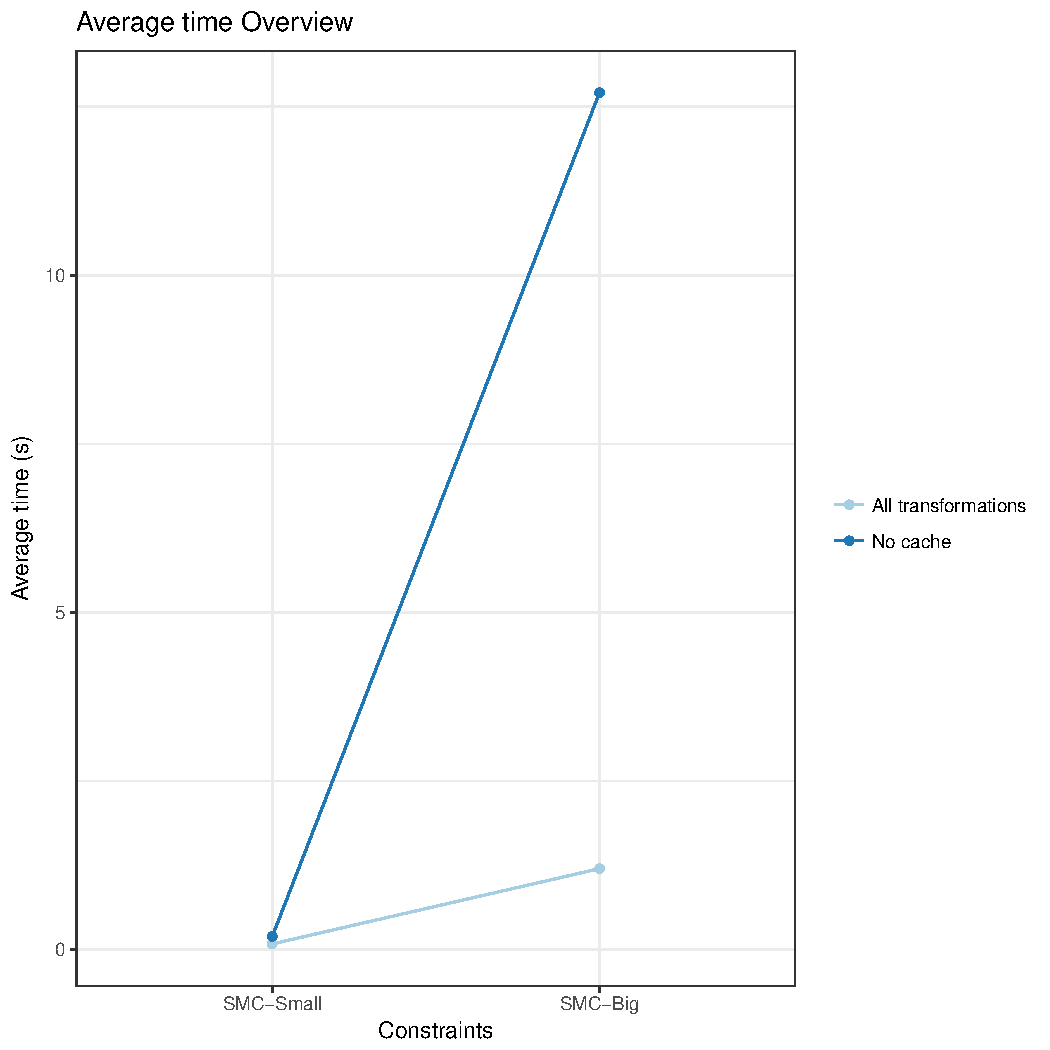
\includegraphics[width=\maxwidth]{figure/overview_averageTime-1} 

\end{knitrout}
\begin{knitrout}
\definecolor{shadecolor}{rgb}{0.969, 0.969, 0.969}\color{fgcolor}
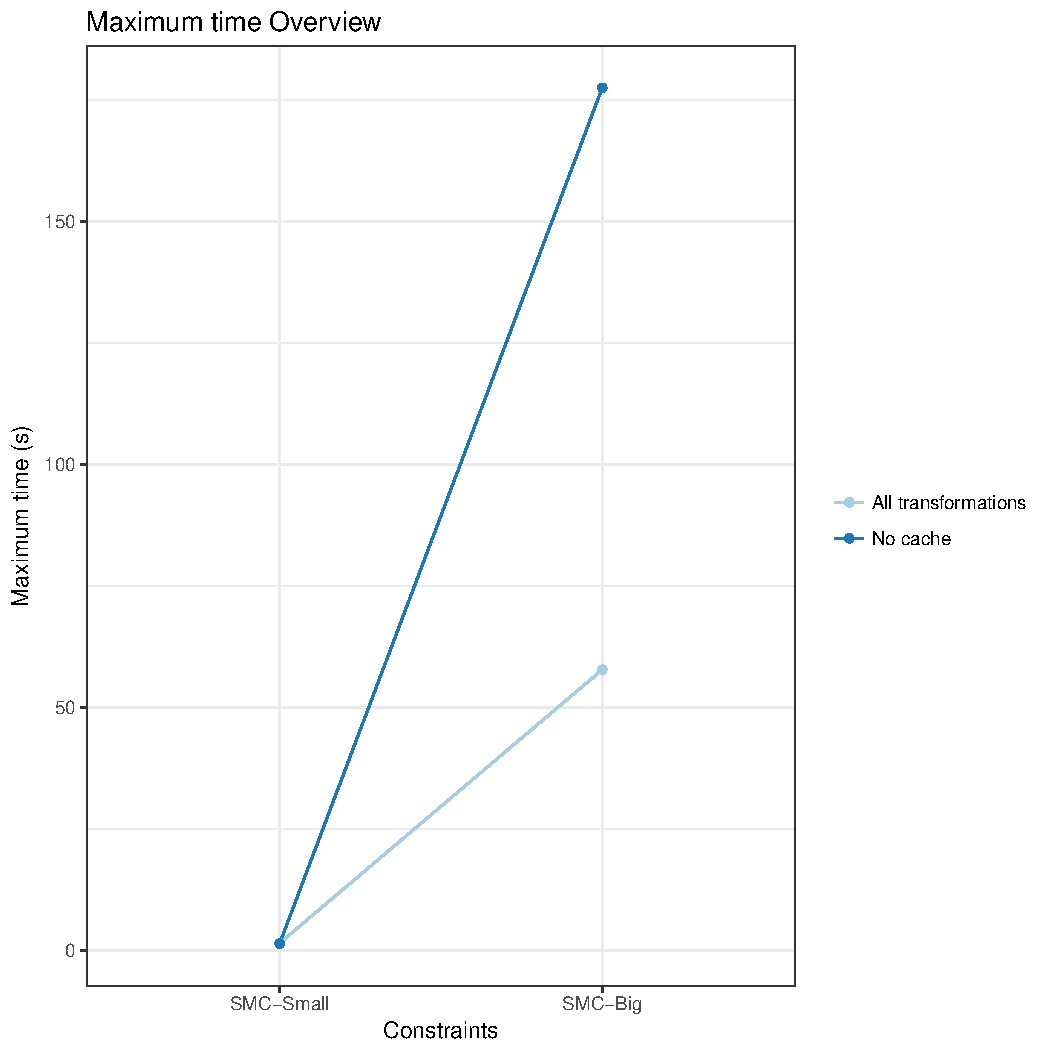
\includegraphics[width=\maxwidth]{figure/overview_maxTime-1} 

\end{knitrout}
\begin{knitrout}
\definecolor{shadecolor}{rgb}{0.969, 0.969, 0.969}\color{fgcolor}
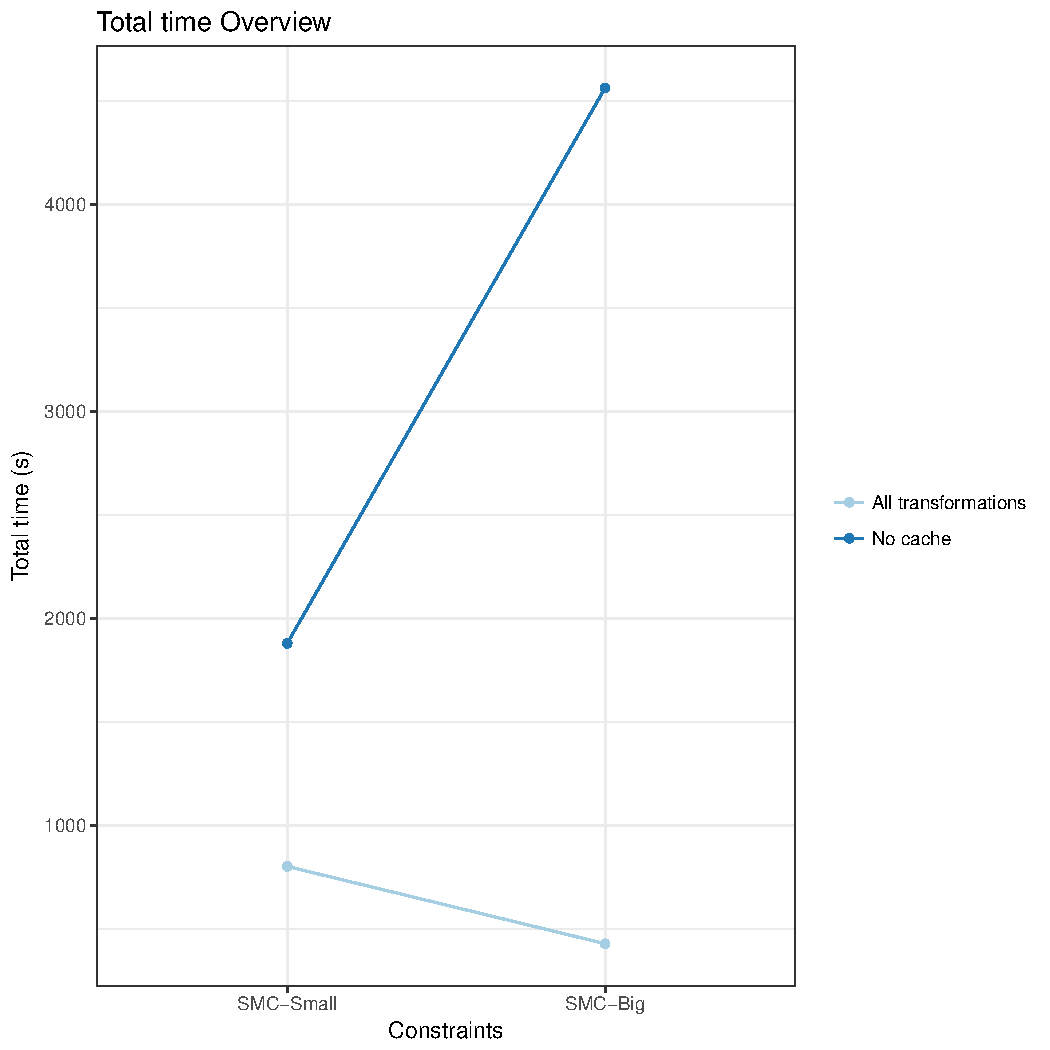
\includegraphics[width=\maxwidth]{figure/overview_sumTime-1} 

\end{knitrout}
\begin{knitrout}
\definecolor{shadecolor}{rgb}{0.969, 0.969, 0.969}\color{fgcolor}
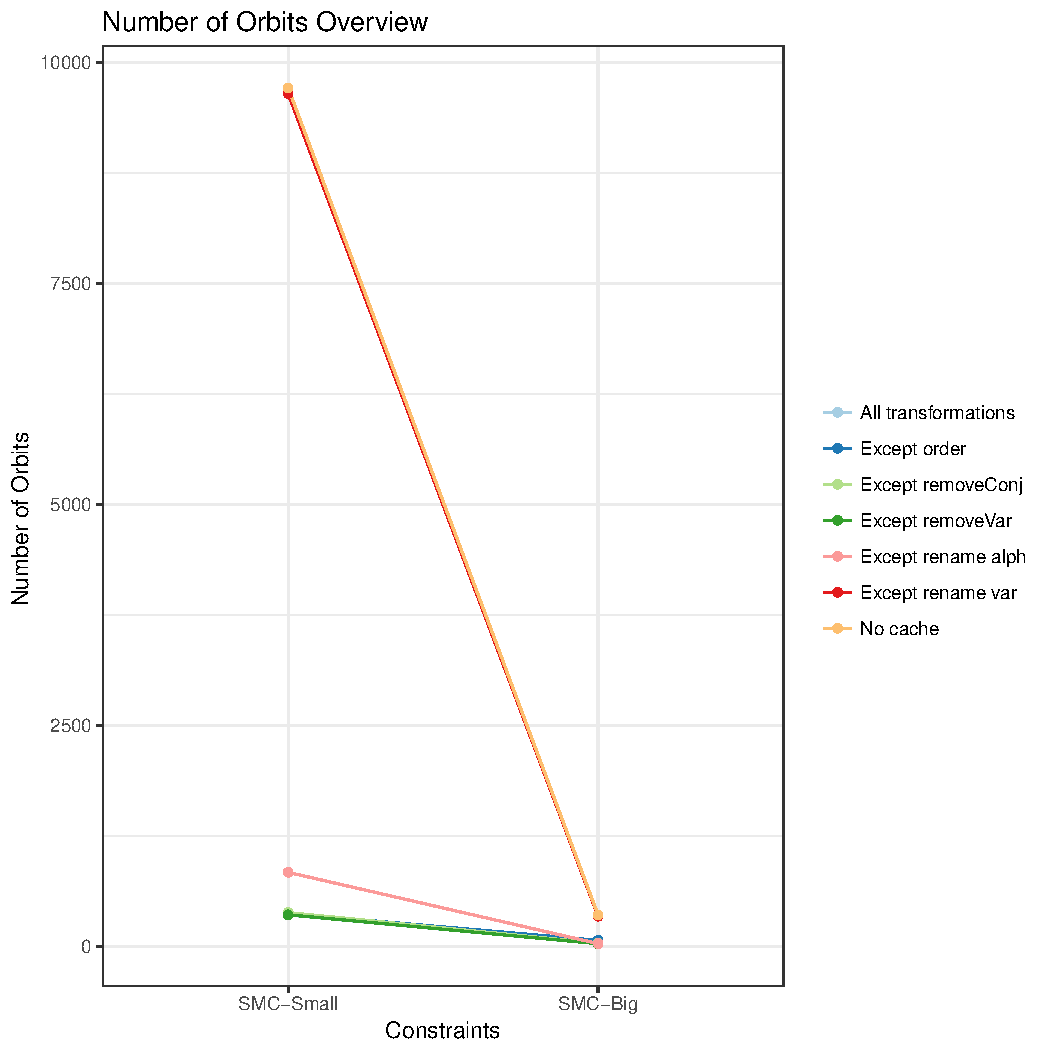
\includegraphics[width=\maxwidth]{figure/overview_orbits-1} 

\end{knitrout}



\subsection{Objects Overview}
\subsubsection{Overview for SMC-Small}
\begin{knitrout}
\definecolor{shadecolor}{rgb}{0.969, 0.969, 0.969}\color{fgcolor}
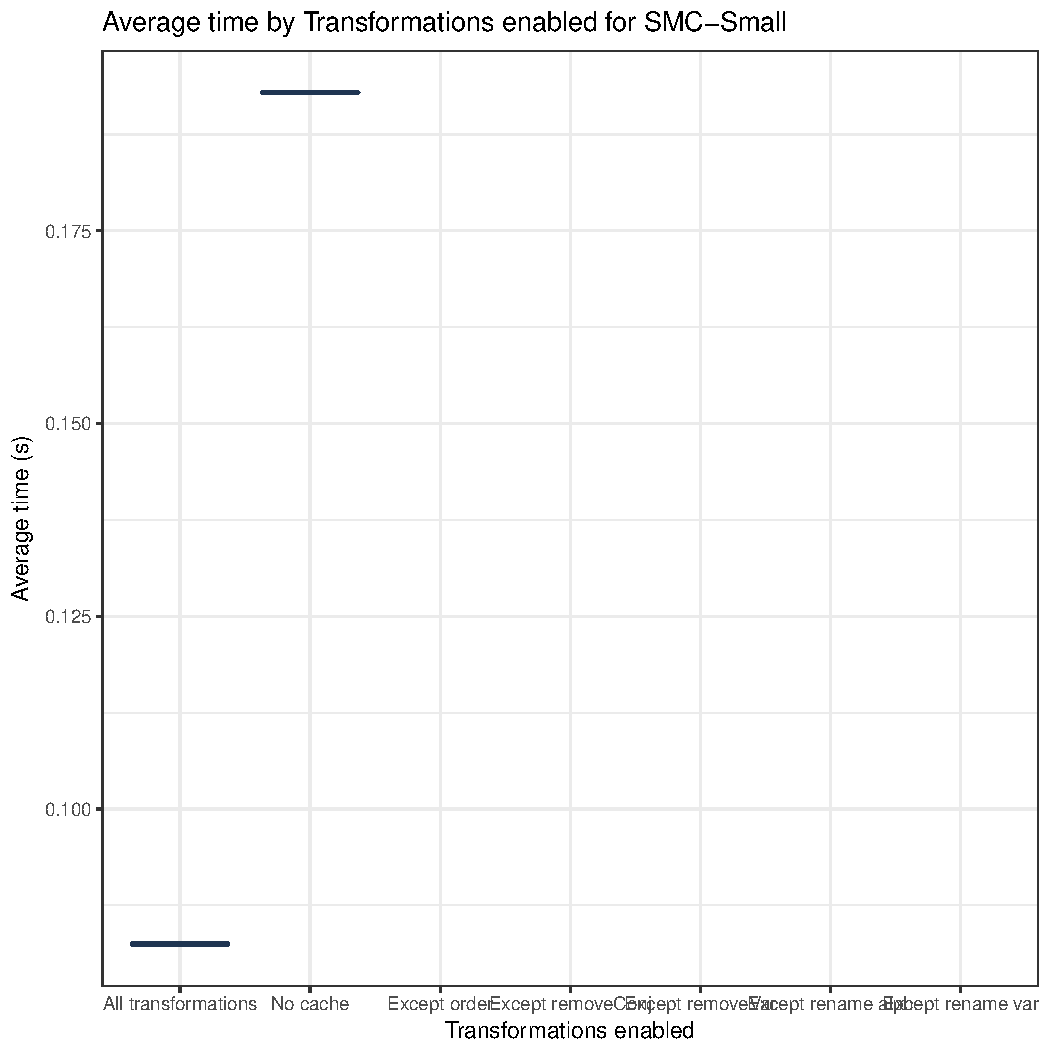
\includegraphics[width=\maxwidth]{figure/small-1} 

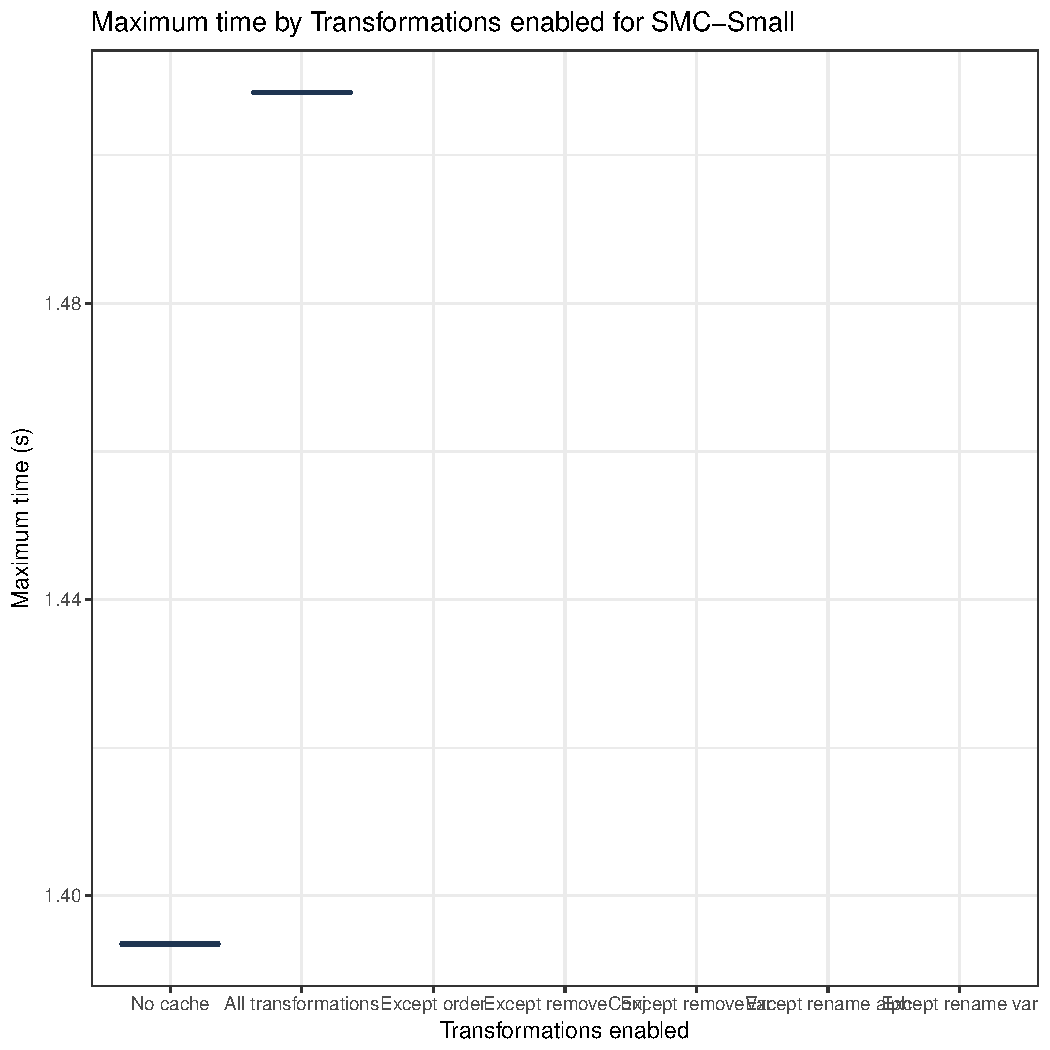
\includegraphics[width=\maxwidth]{figure/small-2} 

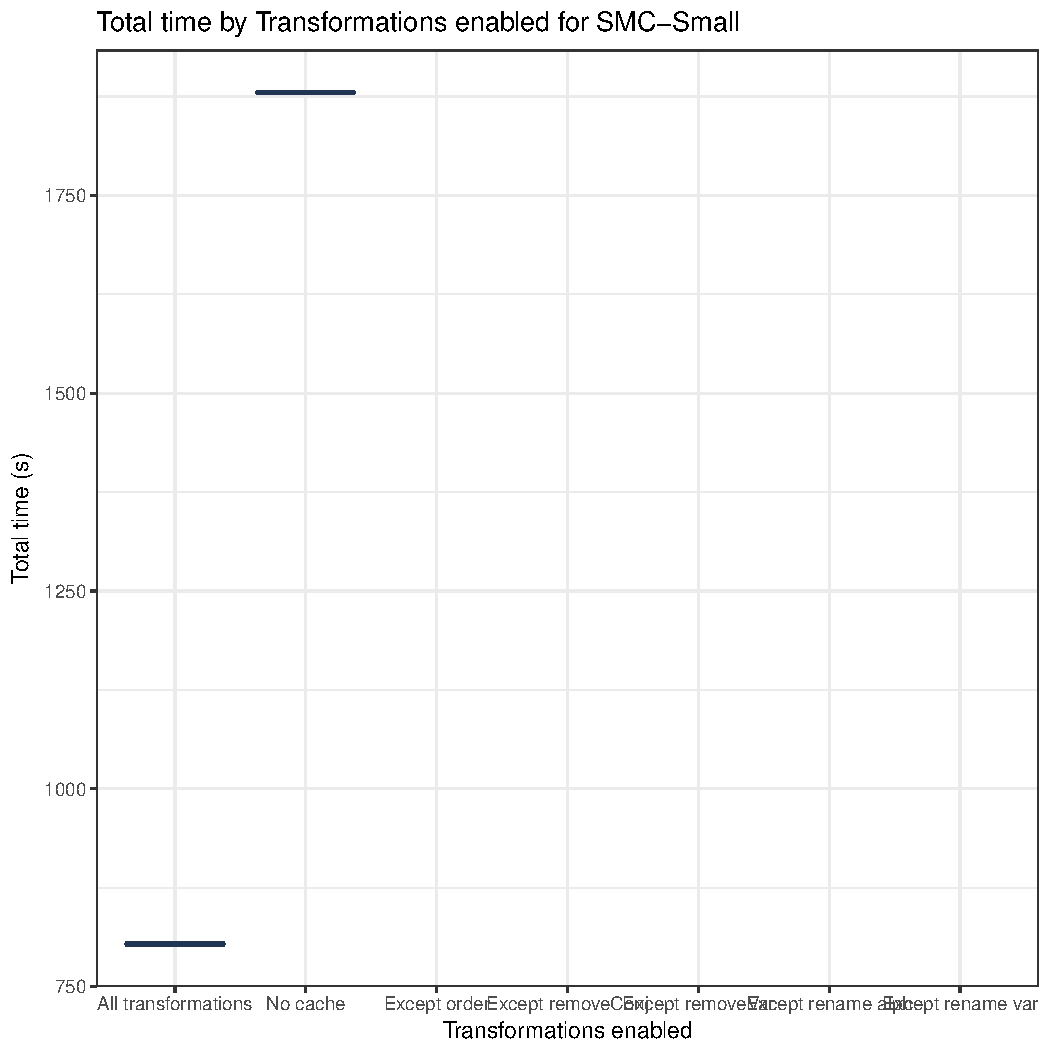
\includegraphics[width=\maxwidth]{figure/small-3} 

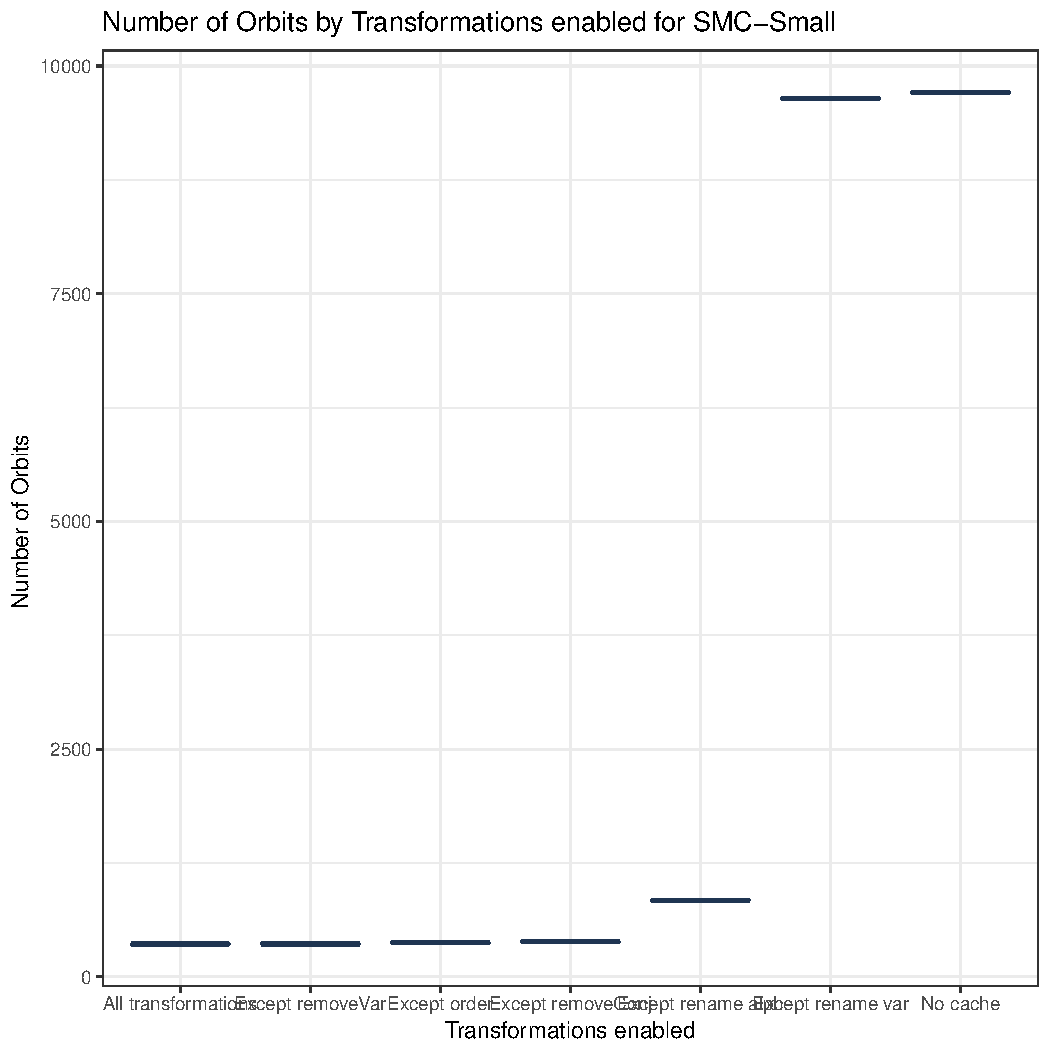
\includegraphics[width=\maxwidth]{figure/small-4} 

\end{knitrout}
\subsubsection{Overview for SMC-Big}
\begin{knitrout}
\definecolor{shadecolor}{rgb}{0.969, 0.969, 0.969}\color{fgcolor}
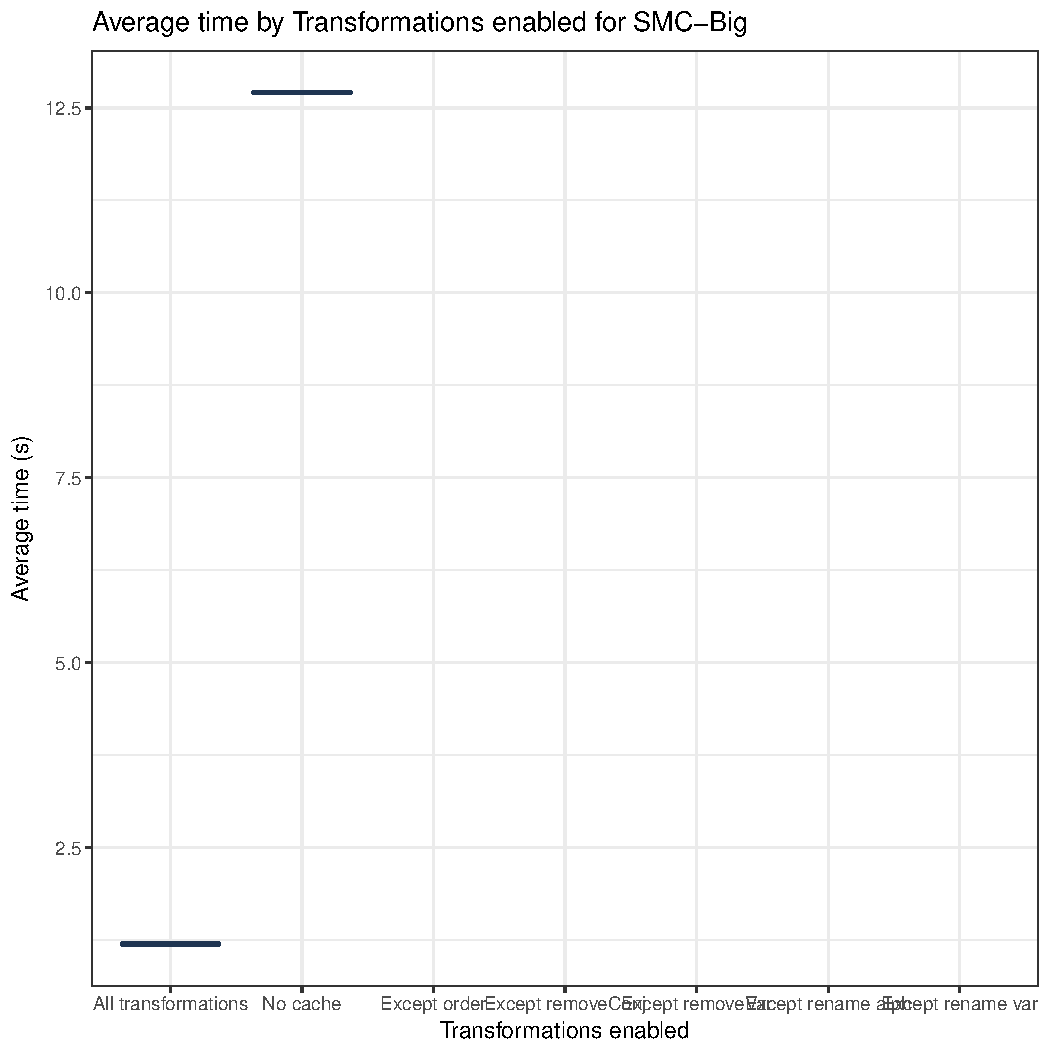
\includegraphics[width=\maxwidth]{figure/big-1} 

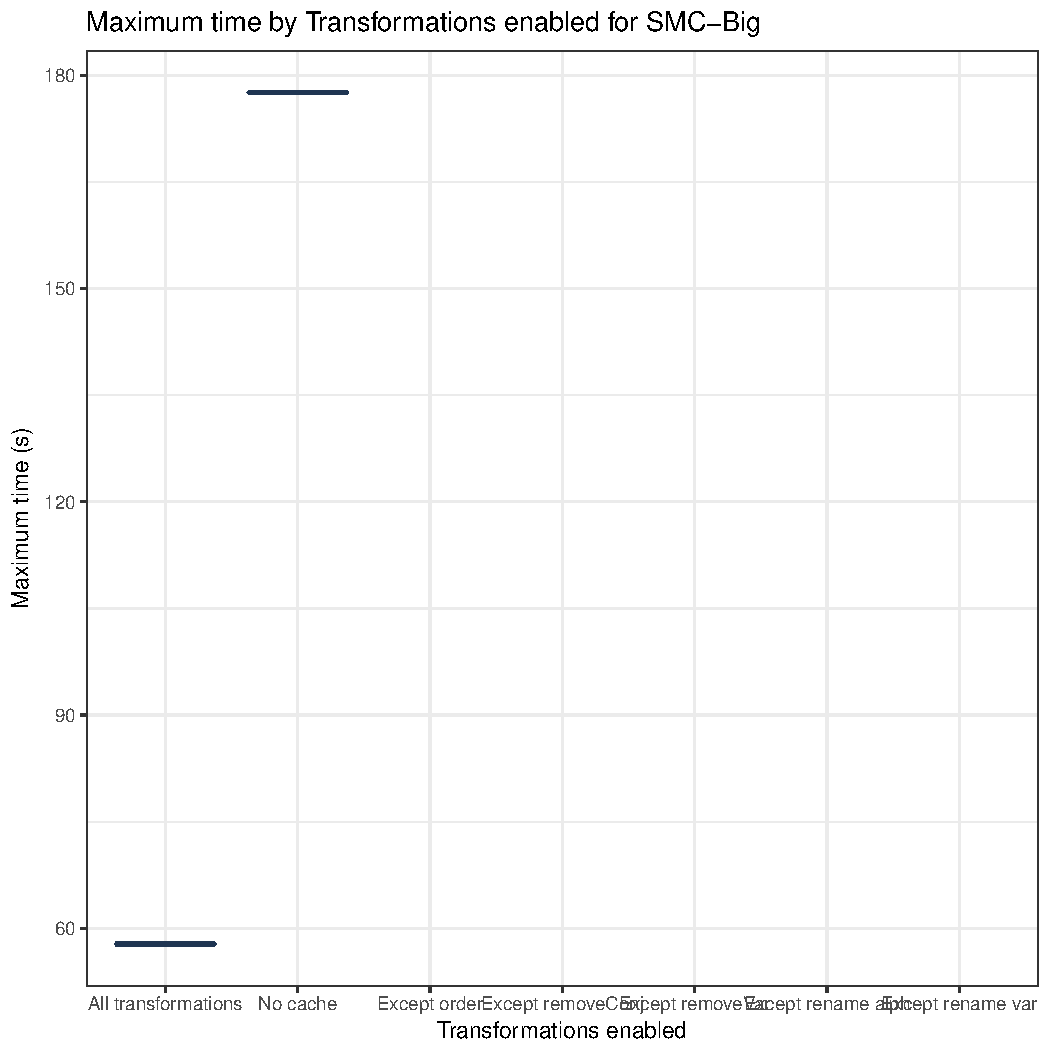
\includegraphics[width=\maxwidth]{figure/big-2} 

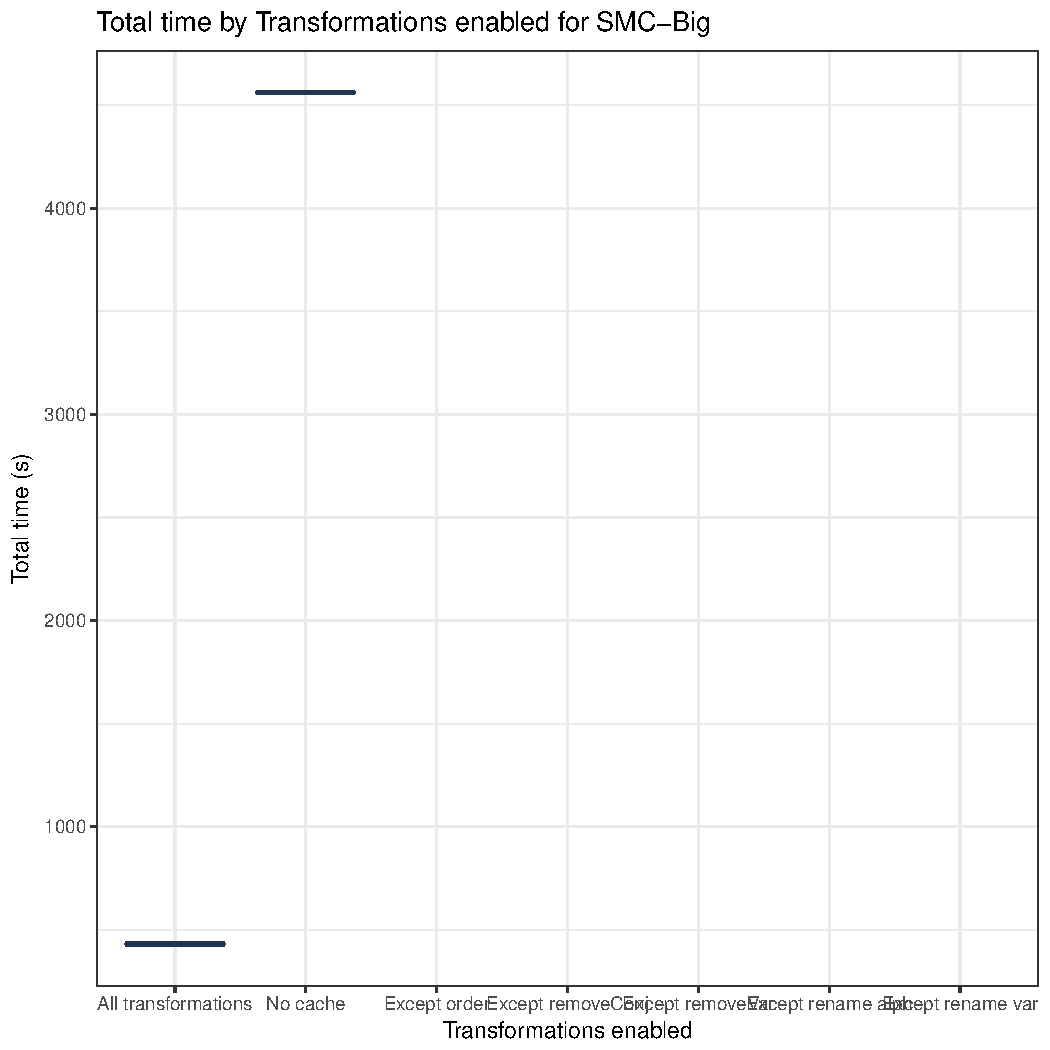
\includegraphics[width=\maxwidth]{figure/big-3} 

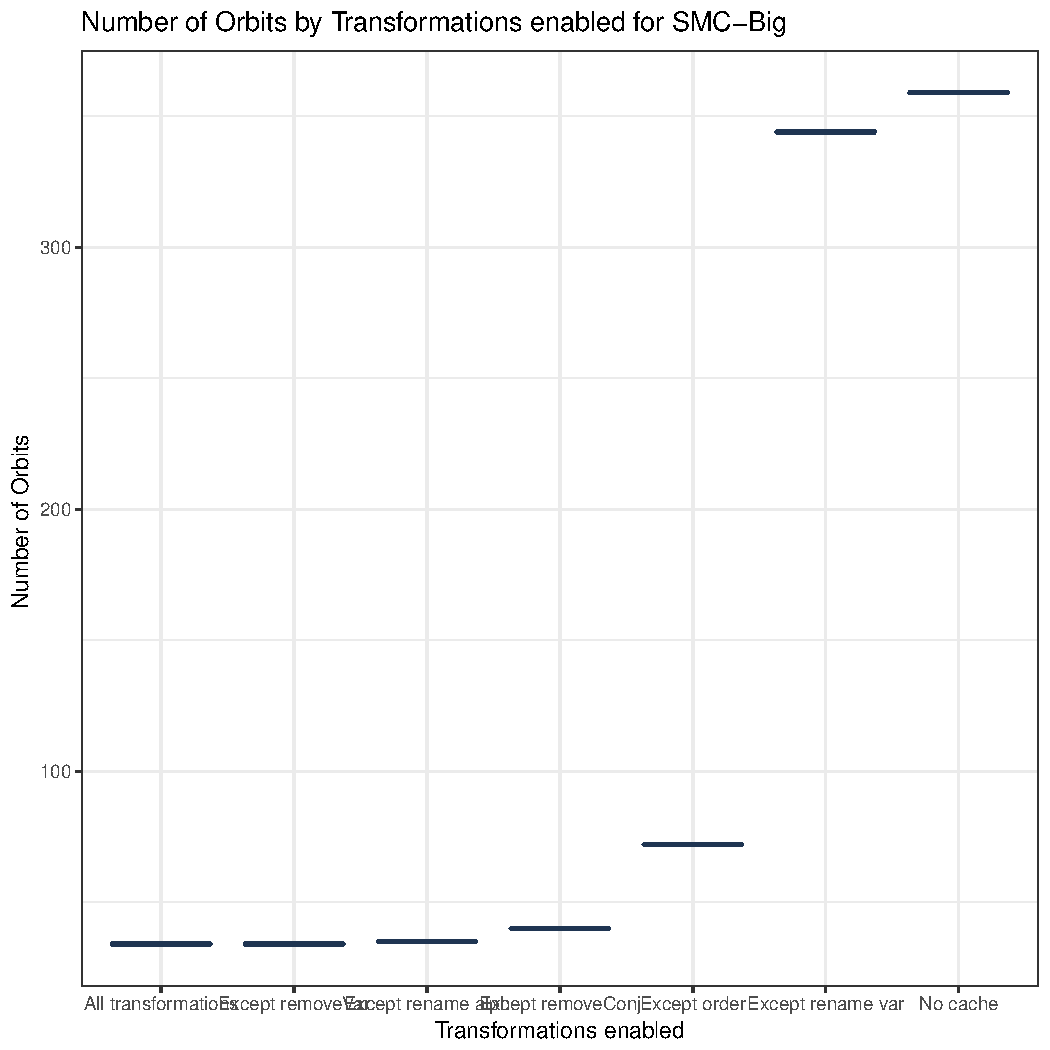
\includegraphics[width=\maxwidth]{figure/big-4} 

\end{knitrout}

\section{Research Hypotheses}

\subsection{RH1: Average time for Cashew is equals than Average time for No Cache}


 
\begin{knitrout}
\definecolor{shadecolor}{rgb}{0.969, 0.969, 0.969}\color{fgcolor}
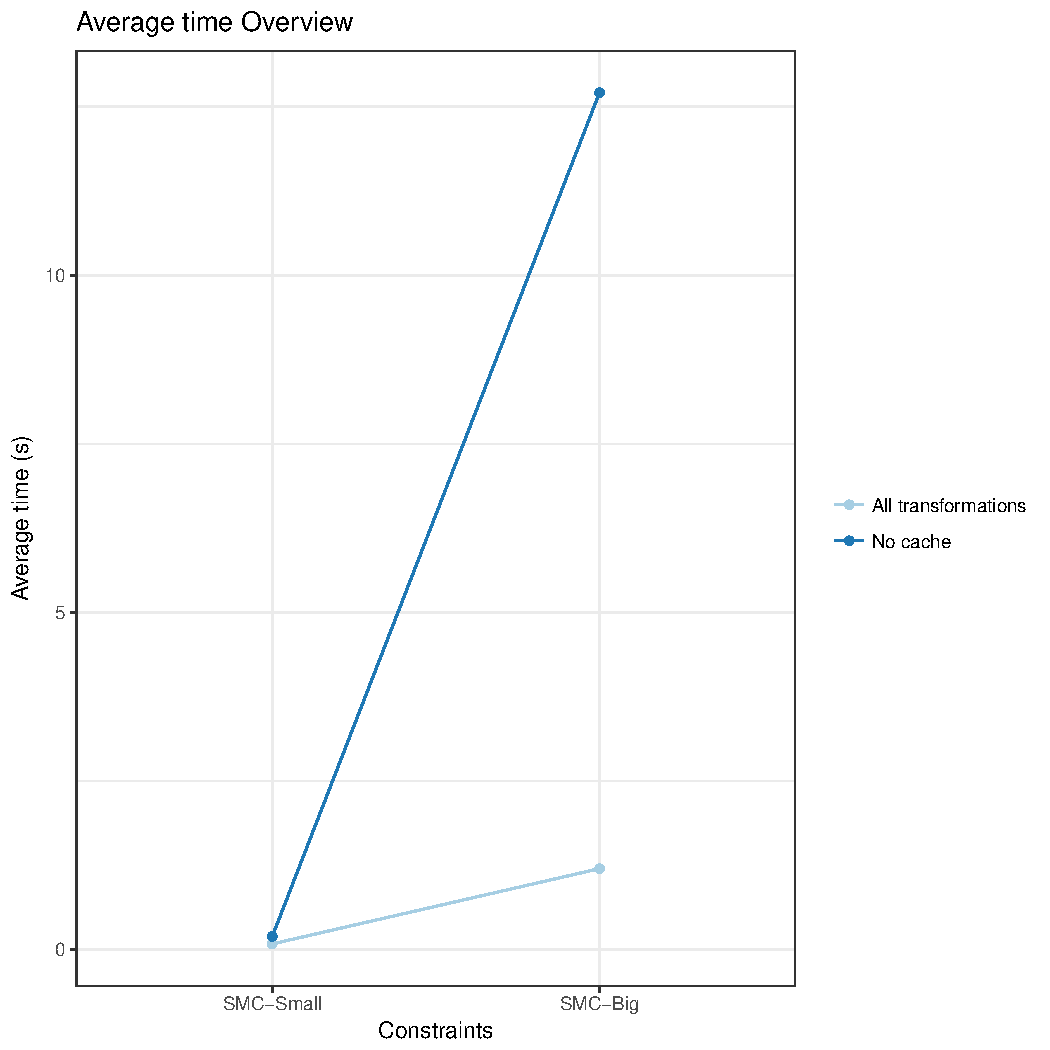
\includegraphics[width=\maxwidth]{figure/overview_RH1-1} 

\end{knitrout}
 	

\subsubsection{RH1.1: Object SMC-Small}

 \textbf{Average time for All transformations}
\begin{knitrout}
\definecolor{shadecolor}{rgb}{0.969, 0.969, 0.969}\color{fgcolor}\begin{kframe}
\begin{verbatim}
## [1] "Sample size:  1"
##    Min. 1st Qu.  Median    Mean 3rd Qu.    Max. 
## 0.08248 0.08248 0.08248 0.08248 0.08248 0.08248
\end{verbatim}


{\ttfamily\noindent\bfseries\color{errorcolor}{\#\# Error in shapiro.test(subset(json\_data, treatment == "{}cashew"{} \& object == : sample size must be between 3 and 5000}}\end{kframe}
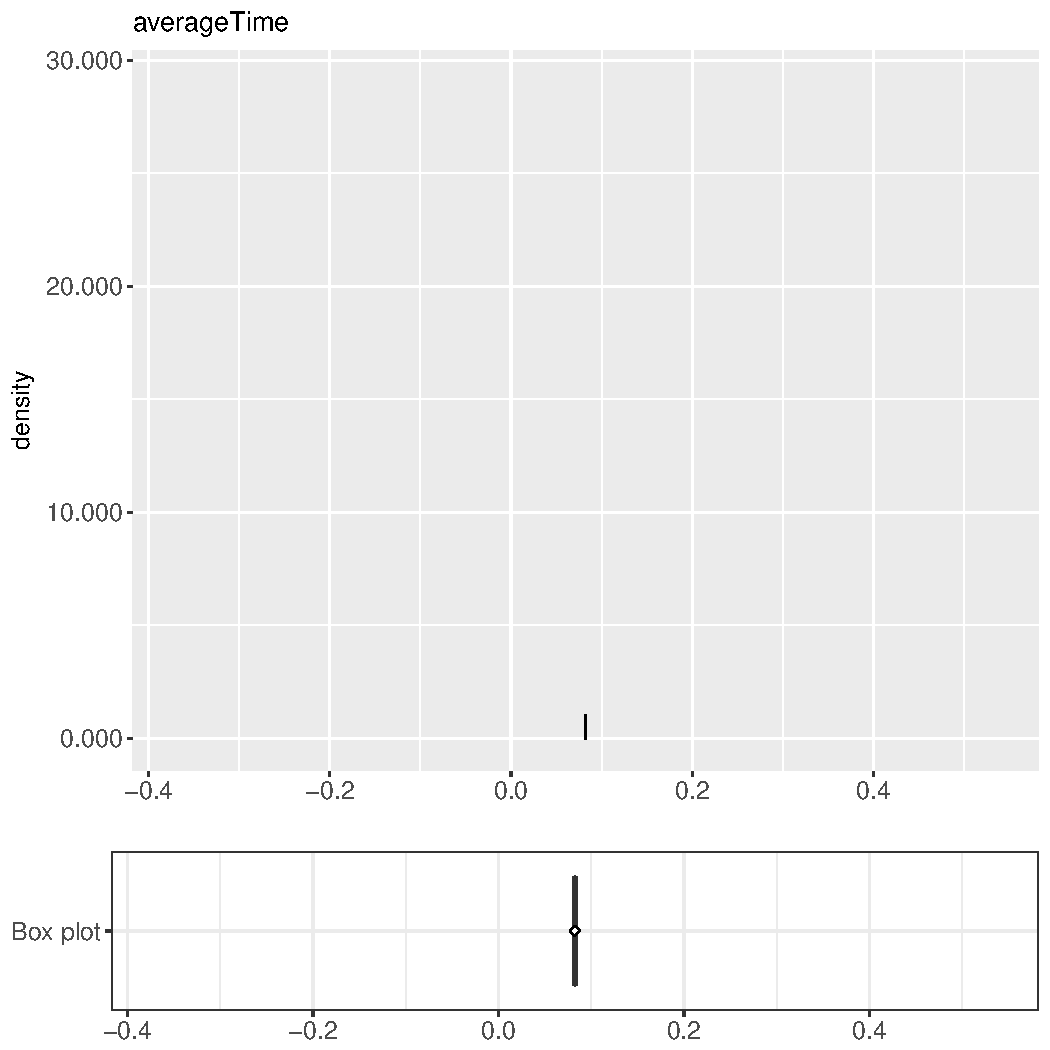
\includegraphics[width=\maxwidth]{figure/RH1_cashew_small-1} 

\end{knitrout}
 \textbf{Average time for No cache}
\begin{knitrout}
\definecolor{shadecolor}{rgb}{0.969, 0.969, 0.969}\color{fgcolor}\begin{kframe}
\begin{verbatim}
## [1] "Sample size:  1"
##    Min. 1st Qu.  Median    Mean 3rd Qu.    Max. 
##  0.1929  0.1929  0.1929  0.1929  0.1929  0.1929
\end{verbatim}


{\ttfamily\noindent\bfseries\color{errorcolor}{\#\# Error in shapiro.test(subset(json\_data, treatment == "{}noCache"{} \& object == : sample size must be between 3 and 5000}}\end{kframe}
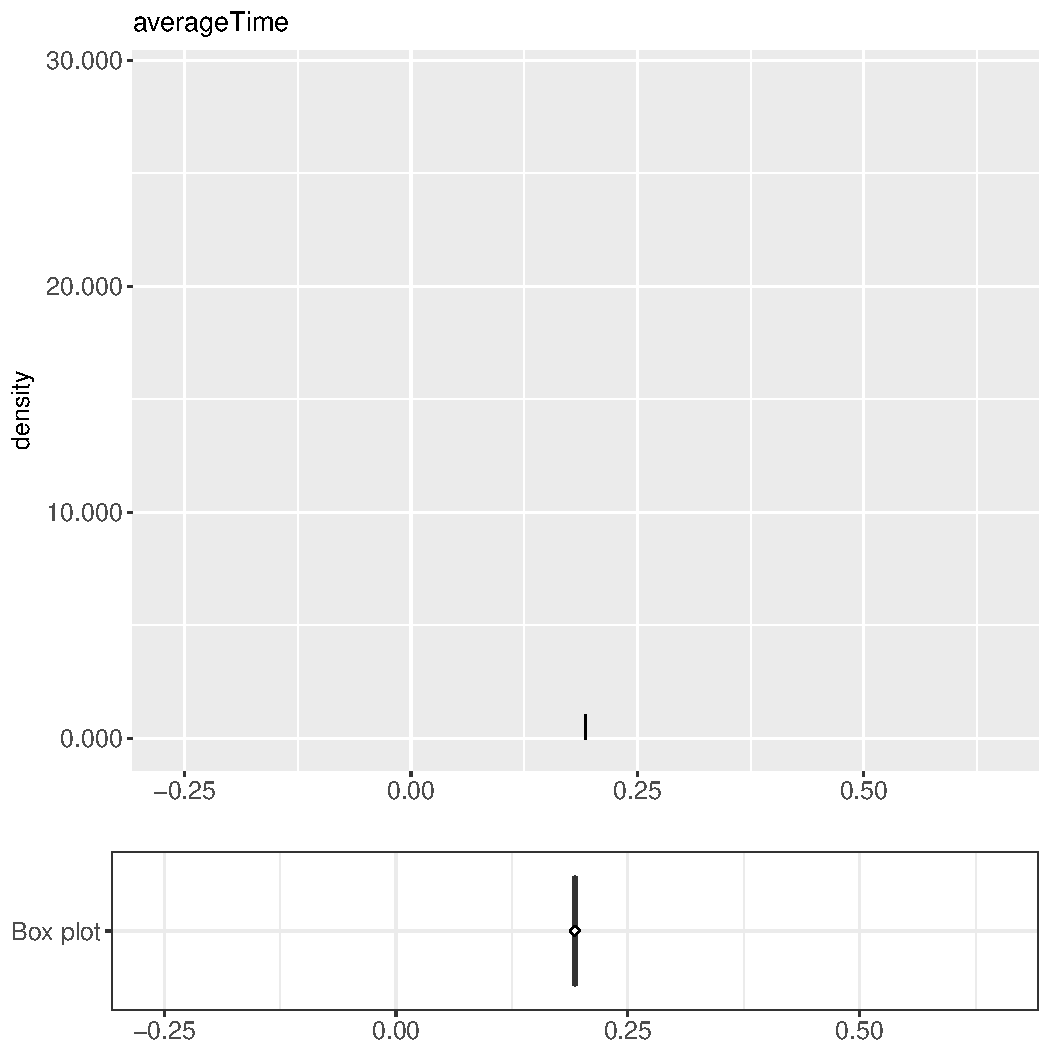
\includegraphics[width=\maxwidth]{figure/RH1_noCache_small-1} 

\end{knitrout}
  
 \textbf{Comparison}
  
\begin{knitrout}
\definecolor{shadecolor}{rgb}{0.969, 0.969, 0.969}\color{fgcolor}
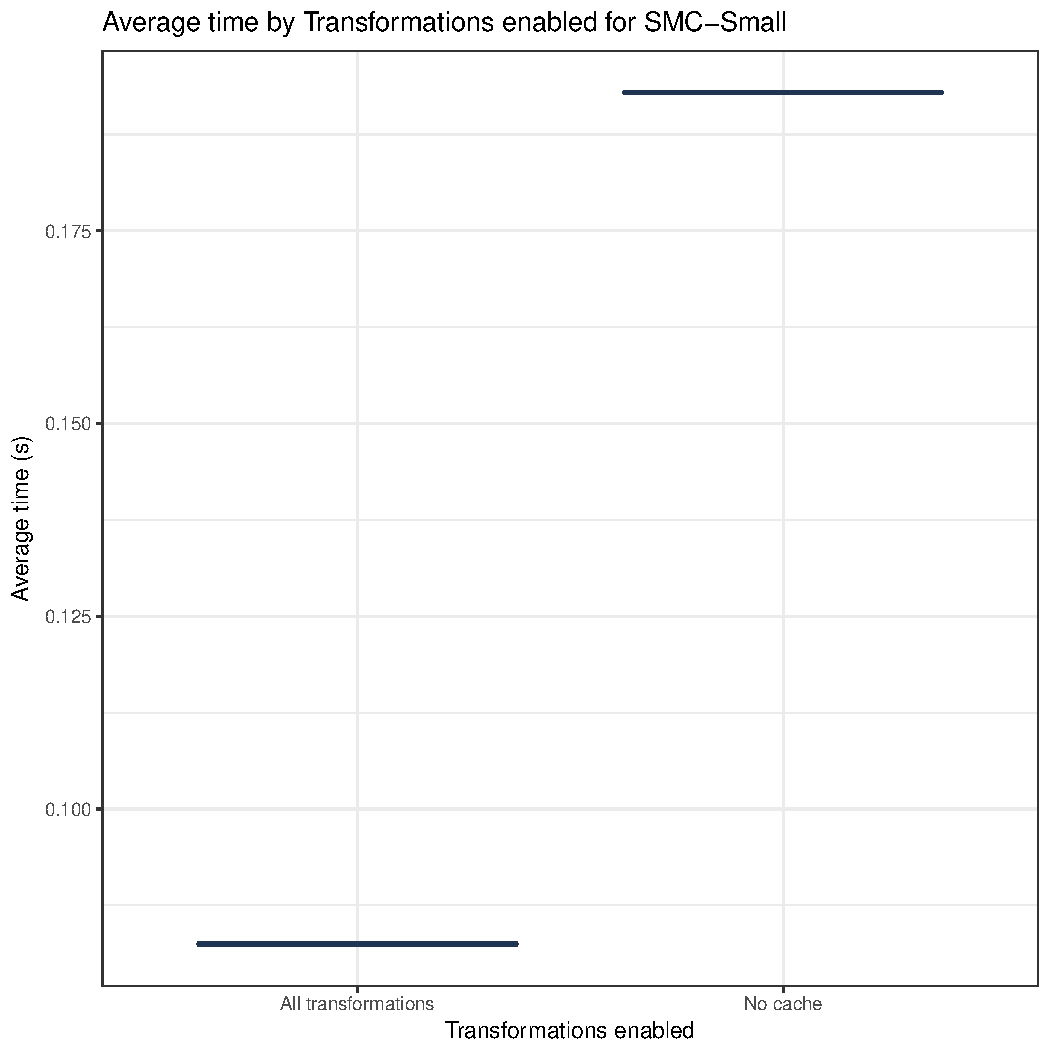
\includegraphics[width=\maxwidth]{figure/RH1_small-1} 
\begin{kframe}

{\ttfamily\noindent\bfseries\color{errorcolor}{\#\# Error in eval(expr, envir, enclos): object 'shap\_cashew\_small' not found}}\begin{verbatim}
## [1] ""
## [1] "Means comparison"
## [1] "Mean Average time for All transformations:  0.0824785"
## [1] "Mean Average time for No cache:  0.192926"
## [1] "Absolute difference:  0.1104475"
## Average time for No cache is  133.910655504162 % greater than 
## Average time for All transformations
\end{verbatim}
\end{kframe}
\end{knitrout}


\subsubsection{RH1.2: Object SMC-Big}

 \textbf{Average time for All transformations}
\begin{knitrout}
\definecolor{shadecolor}{rgb}{0.969, 0.969, 0.969}\color{fgcolor}\begin{kframe}
\begin{verbatim}
## [1] "Sample size:  1"
##    Min. 1st Qu.  Median    Mean 3rd Qu.    Max. 
##   1.199   1.199   1.199   1.199   1.199   1.199
\end{verbatim}


{\ttfamily\noindent\bfseries\color{errorcolor}{\#\# Error in shapiro.test(subset(json\_data, treatment == "{}cashew"{} \& object == : sample size must be between 3 and 5000}}\end{kframe}
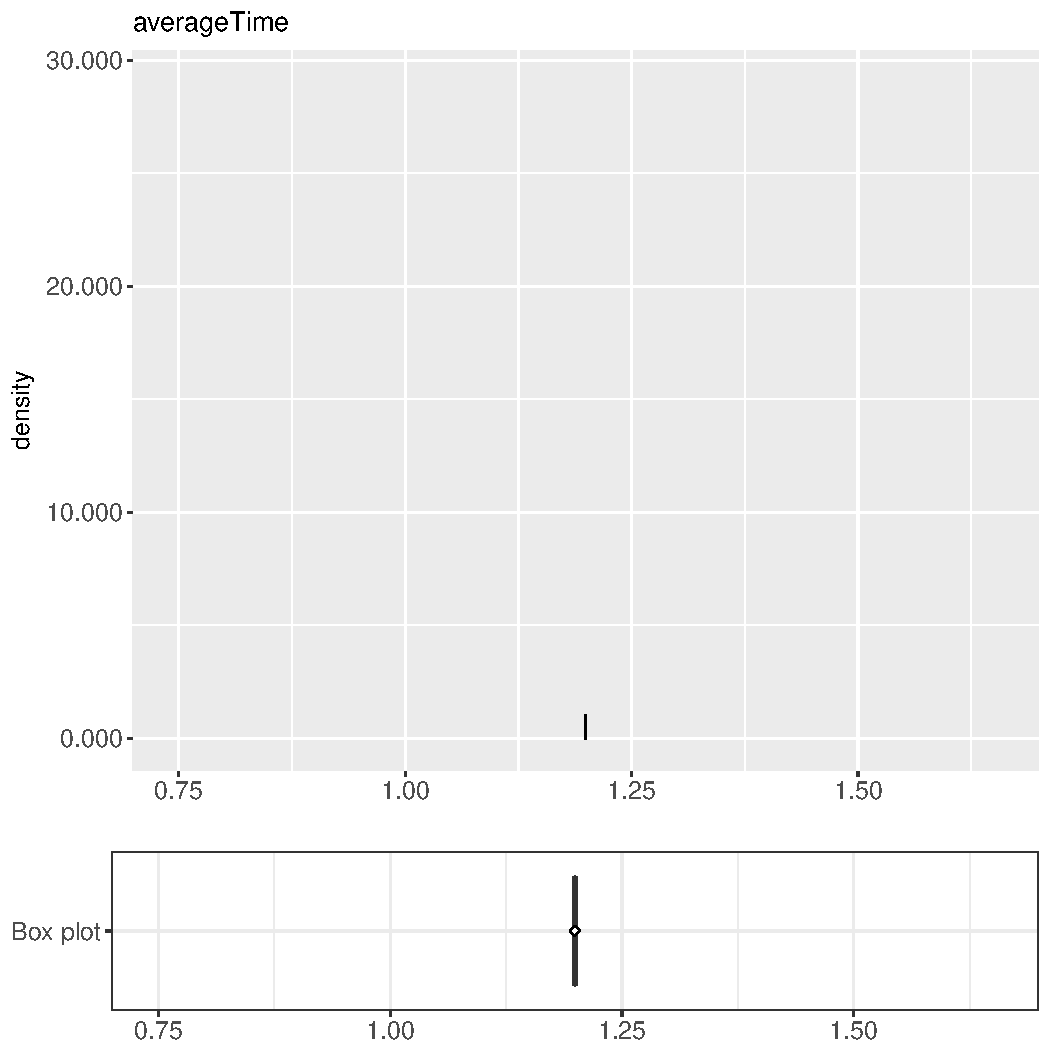
\includegraphics[width=\maxwidth]{figure/RH1_cashew_big-1} 

\end{knitrout}
 \textbf{Average time for No cache}
\begin{knitrout}
\definecolor{shadecolor}{rgb}{0.969, 0.969, 0.969}\color{fgcolor}\begin{kframe}
\begin{verbatim}
## [1] "Sample size:  1"
##    Min. 1st Qu.  Median    Mean 3rd Qu.    Max. 
##   12.71   12.71   12.71   12.71   12.71   12.71
\end{verbatim}


{\ttfamily\noindent\bfseries\color{errorcolor}{\#\# Error in shapiro.test(subset(json\_data, treatment == "{}noCache"{} \& object == : sample size must be between 3 and 5000}}\end{kframe}
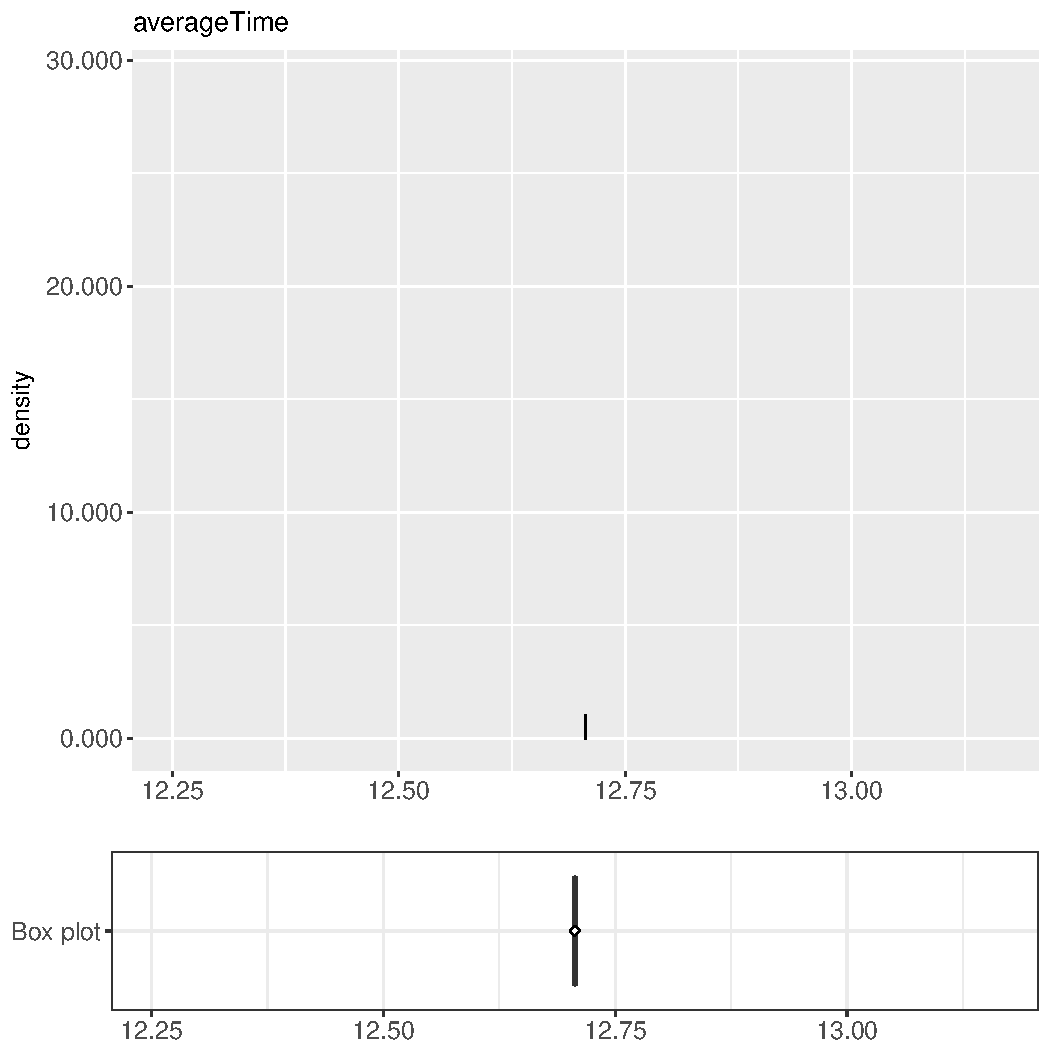
\includegraphics[width=\maxwidth]{figure/RH1_noCache_big-1} 

\end{knitrout}
  
 \textbf{Comparison}
  
\begin{knitrout}
\definecolor{shadecolor}{rgb}{0.969, 0.969, 0.969}\color{fgcolor}
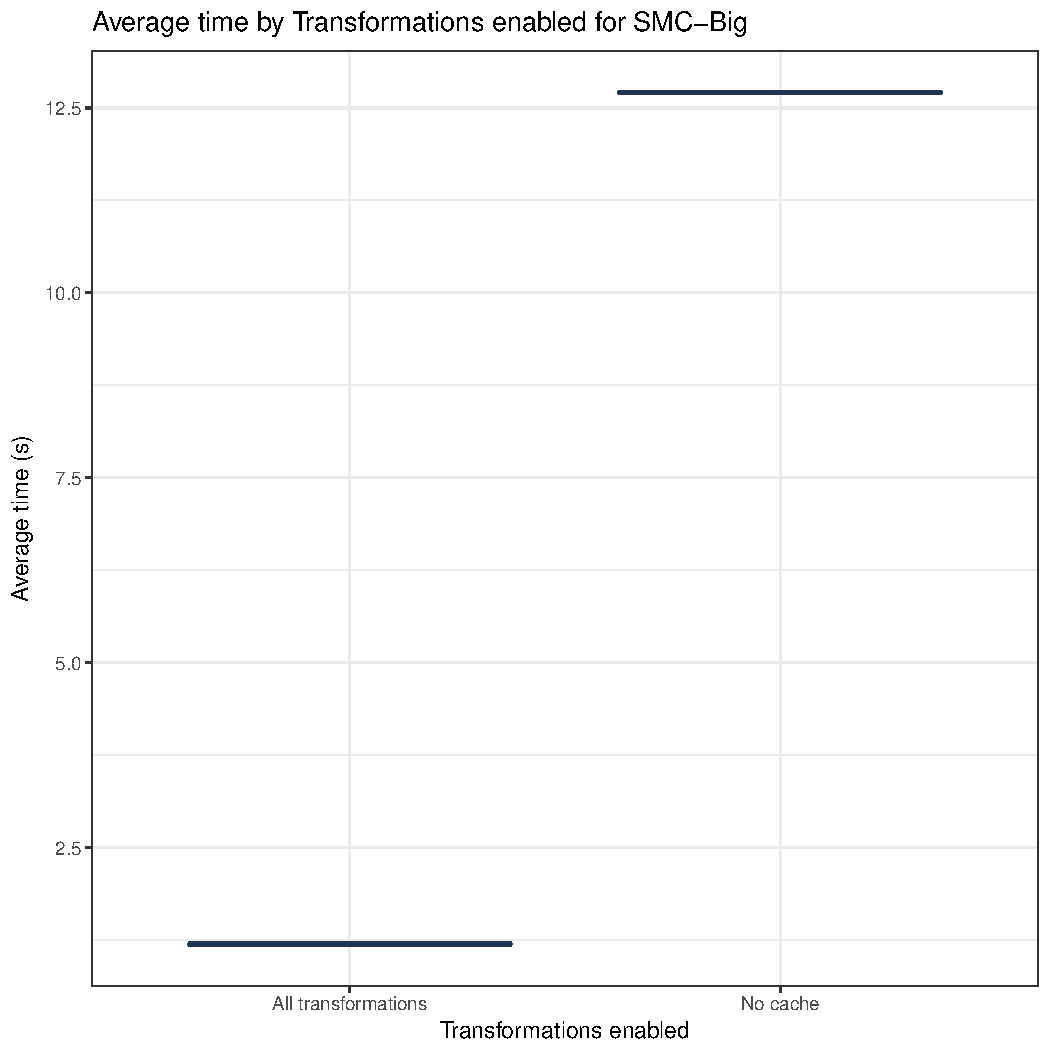
\includegraphics[width=\maxwidth]{figure/RH1_big-1} 
\begin{kframe}

{\ttfamily\noindent\bfseries\color{errorcolor}{\#\# Error in eval(expr, envir, enclos): object 'shap\_cashew\_big' not found}}\begin{verbatim}
## [1] ""
## [1] "Means comparison"
## [1] "Mean Average time for All transformations:  1.19926"
## [1] "Mean Average time for No cache:  12.7065"
## [1] "Absolute difference:  11.50724"
## Average time for No cache is  959.528375831763 % greater than 
## Average time for All transformations
\end{verbatim}
\end{kframe}
\end{knitrout}


 

	
	\subsubsection{RH1 Results: Average time All transformations = No cache}
	
	
	\begin{table}[H]
	\centering
	\caption{RH1 Results per Object}
	\begin{tabular}{ll}
	\textbf{SMC-Small} & Inconclusive \\
	\textbf{SMC-Big} & Inconclusive \\
	\end{tabular}
	\end{table}

	\begin{table}[H]
	\centering
	\caption{RH1 Results Summary}
	\begin{tabular}{ll}
	\textbf{All transformations \textless{} No cache:}& 0\% \\
	\textbf{All transformations \textgreater{} No cache:}& 0\%\\
	\textbf{All transformations:} & 0\%\\
	\textbf{No cache:} & 0\%\\
	\textbf{None:}& 0\%\\
	\textbf{Inconclusive:}& 100\%
			
	
	\end{tabular}
	\end{table}
	
	
	



\subsection{RH2: Maximum time for Cashew is equals than Average time for No Cache}


 
\begin{knitrout}
\definecolor{shadecolor}{rgb}{0.969, 0.969, 0.969}\color{fgcolor}
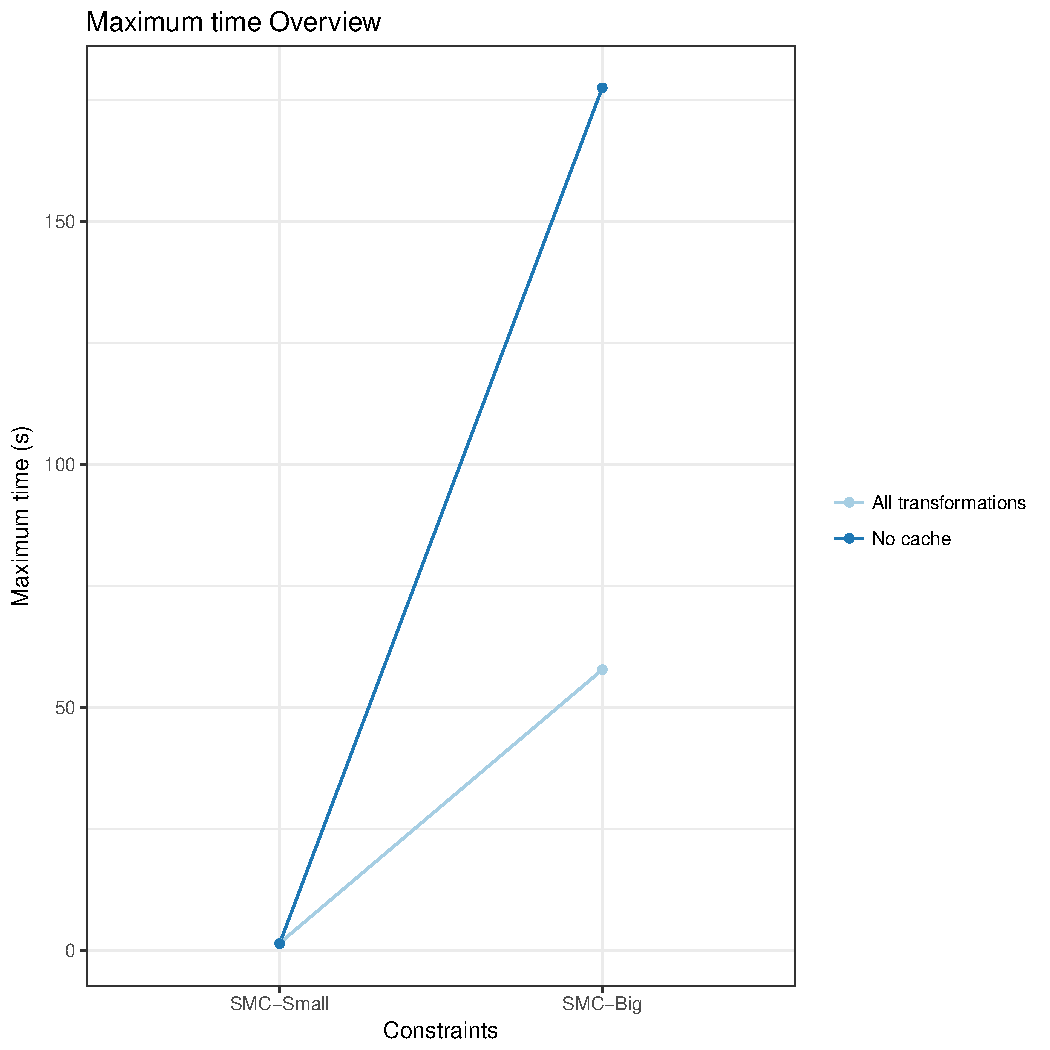
\includegraphics[width=\maxwidth]{figure/overview_RH2-1} 

\end{knitrout}
 	

\subsubsection{RH2.1: Object SMC-Small}

 \textbf{Maximum time for All transformations}
\begin{knitrout}
\definecolor{shadecolor}{rgb}{0.969, 0.969, 0.969}\color{fgcolor}\begin{kframe}
\begin{verbatim}
## [1] "Sample size:  1"
##    Min. 1st Qu.  Median    Mean 3rd Qu.    Max. 
##   1.508   1.508   1.508   1.508   1.508   1.508
\end{verbatim}


{\ttfamily\noindent\bfseries\color{errorcolor}{\#\# Error in shapiro.test(subset(json\_data, treatment == "{}cashew"{} \& object == : sample size must be between 3 and 5000}}\end{kframe}
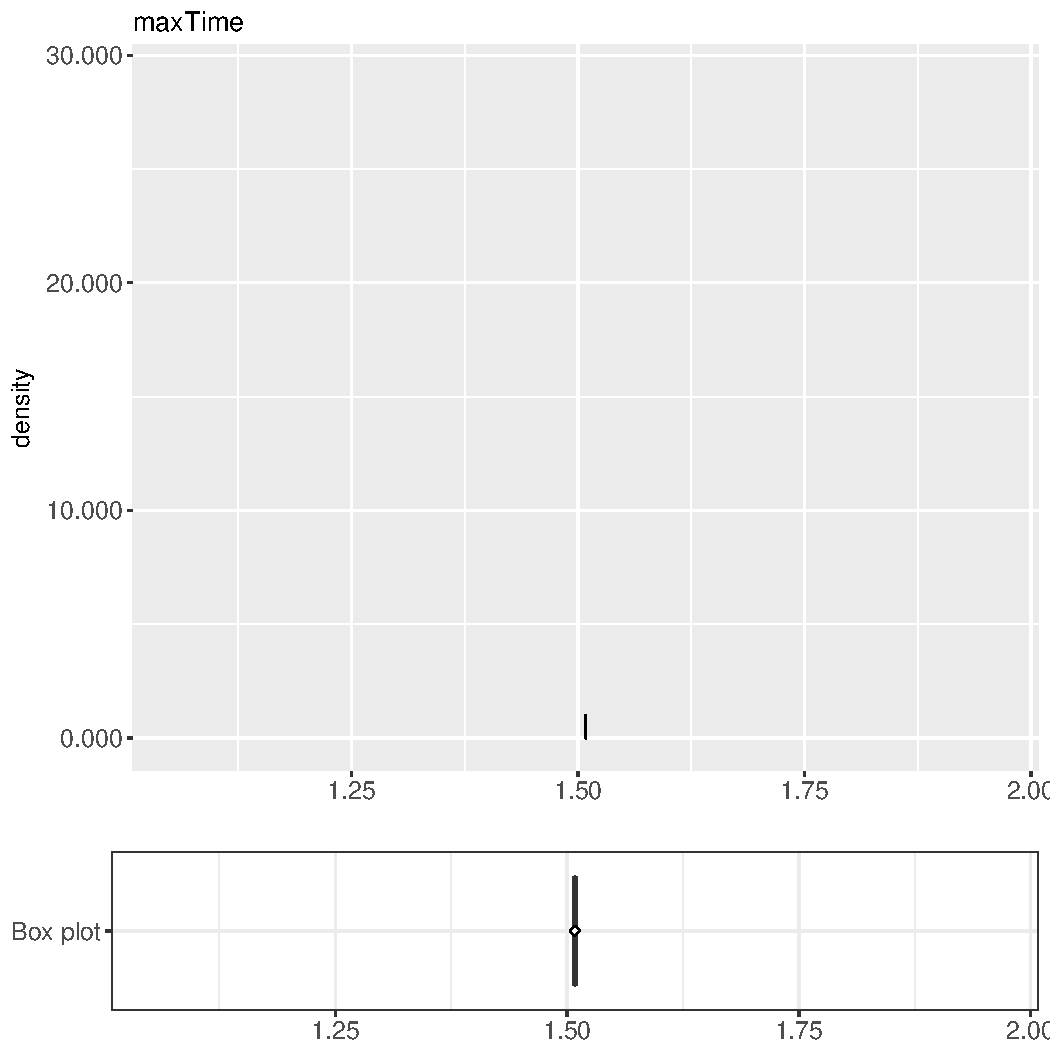
\includegraphics[width=\maxwidth]{figure/RH2_cashew_small-1} 

\end{knitrout}
 \textbf{Maximum time for No cache}
\begin{knitrout}
\definecolor{shadecolor}{rgb}{0.969, 0.969, 0.969}\color{fgcolor}\begin{kframe}
\begin{verbatim}
## [1] "Sample size:  1"
##    Min. 1st Qu.  Median    Mean 3rd Qu.    Max. 
##   1.393   1.393   1.393   1.393   1.393   1.393
\end{verbatim}


{\ttfamily\noindent\bfseries\color{errorcolor}{\#\# Error in shapiro.test(subset(json\_data, treatment == "{}noCache"{} \& object == : sample size must be between 3 and 5000}}\end{kframe}
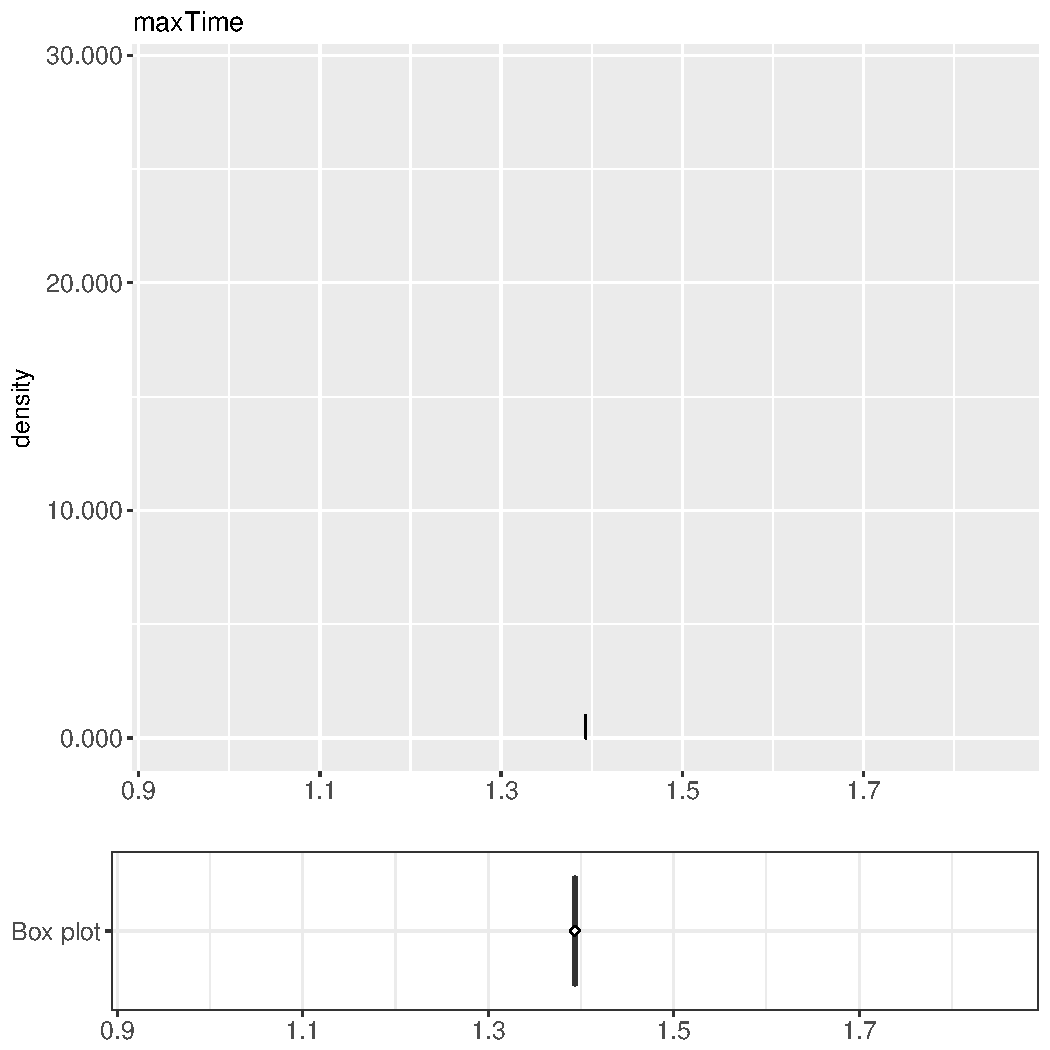
\includegraphics[width=\maxwidth]{figure/RH2_noCache_small-1} 

\end{knitrout}
  
 \textbf{Comparison}
  
\begin{knitrout}
\definecolor{shadecolor}{rgb}{0.969, 0.969, 0.969}\color{fgcolor}
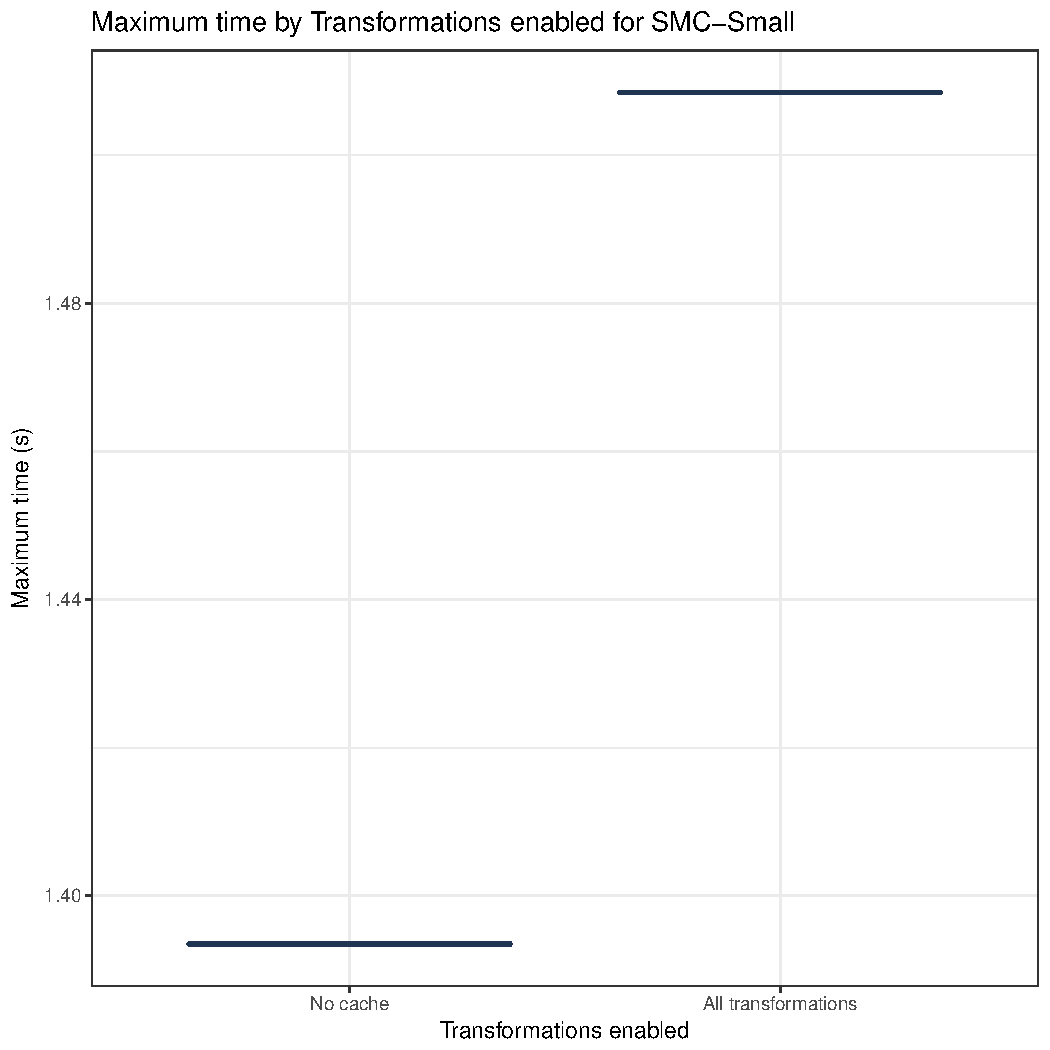
\includegraphics[width=\maxwidth]{figure/RH2_small-1} 
\begin{kframe}

{\ttfamily\noindent\bfseries\color{errorcolor}{\#\# Error in eval(expr, envir, enclos): object 'shap\_cashew\_small' not found}}\begin{verbatim}
## [1] ""
## [1] "Means comparison"
## [1] "Mean Maximum time for All transformations:  1.50848"
## [1] "Mean Maximum time for No cache:  1.39348"
## [1] "Absolute difference:  0.115"
## Maximum time for All transformations is  8.25271980939805 % greater than 
##  Maximum time for No cache
\end{verbatim}
\end{kframe}
\end{knitrout}


\subsubsection{RH2.2: Object SMC-Big}

 \textbf{Maximum time for All transformations}
\begin{knitrout}
\definecolor{shadecolor}{rgb}{0.969, 0.969, 0.969}\color{fgcolor}\begin{kframe}
\begin{verbatim}
## [1] "Sample size:  1"
##    Min. 1st Qu.  Median    Mean 3rd Qu.    Max. 
##   57.79   57.79   57.79   57.79   57.79   57.79
\end{verbatim}


{\ttfamily\noindent\bfseries\color{errorcolor}{\#\# Error in shapiro.test(subset(json\_data, treatment == "{}cashew"{} \& object == : sample size must be between 3 and 5000}}\end{kframe}
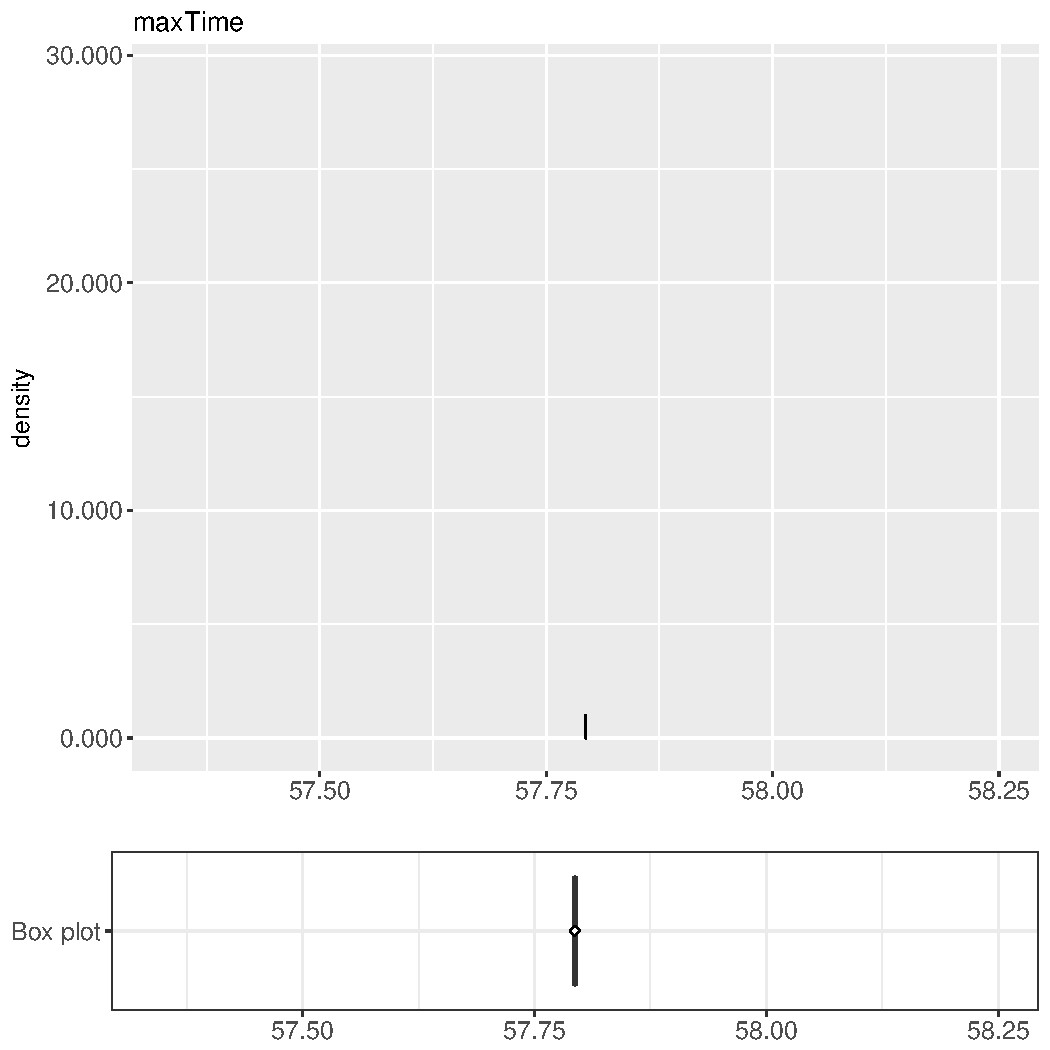
\includegraphics[width=\maxwidth]{figure/RH2_cashew_big-1} 

\end{knitrout}
 \textbf{Maximum time for No cache}
\begin{knitrout}
\definecolor{shadecolor}{rgb}{0.969, 0.969, 0.969}\color{fgcolor}\begin{kframe}
\begin{verbatim}
## [1] "Sample size:  1"
##    Min. 1st Qu.  Median    Mean 3rd Qu.    Max. 
##   177.6   177.6   177.6   177.6   177.6   177.6
\end{verbatim}


{\ttfamily\noindent\bfseries\color{errorcolor}{\#\# Error in shapiro.test(subset(json\_data, treatment == "{}noCache"{} \& object == : sample size must be between 3 and 5000}}\end{kframe}
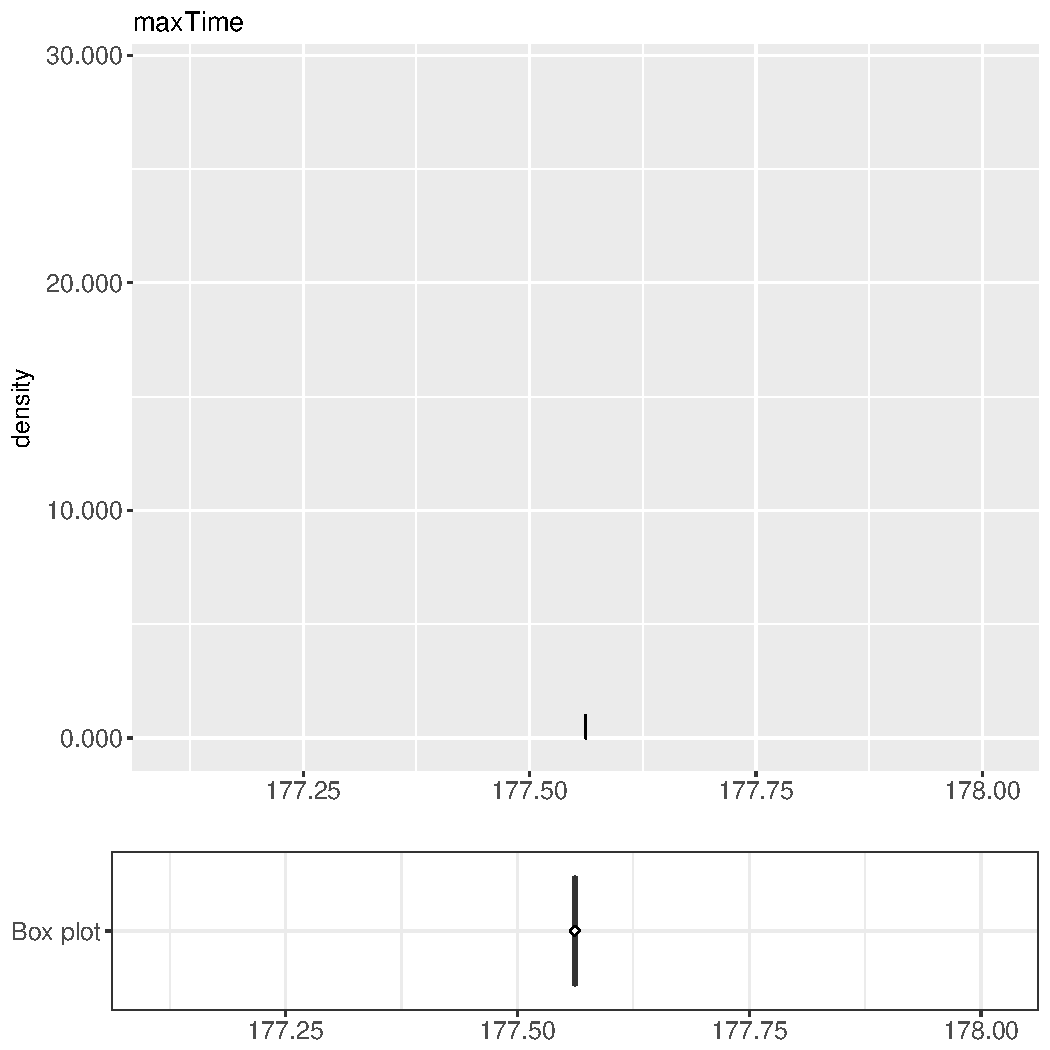
\includegraphics[width=\maxwidth]{figure/RH2_noCache_big-1} 

\end{knitrout}
  
 \textbf{Comparison}
  
\begin{knitrout}
\definecolor{shadecolor}{rgb}{0.969, 0.969, 0.969}\color{fgcolor}
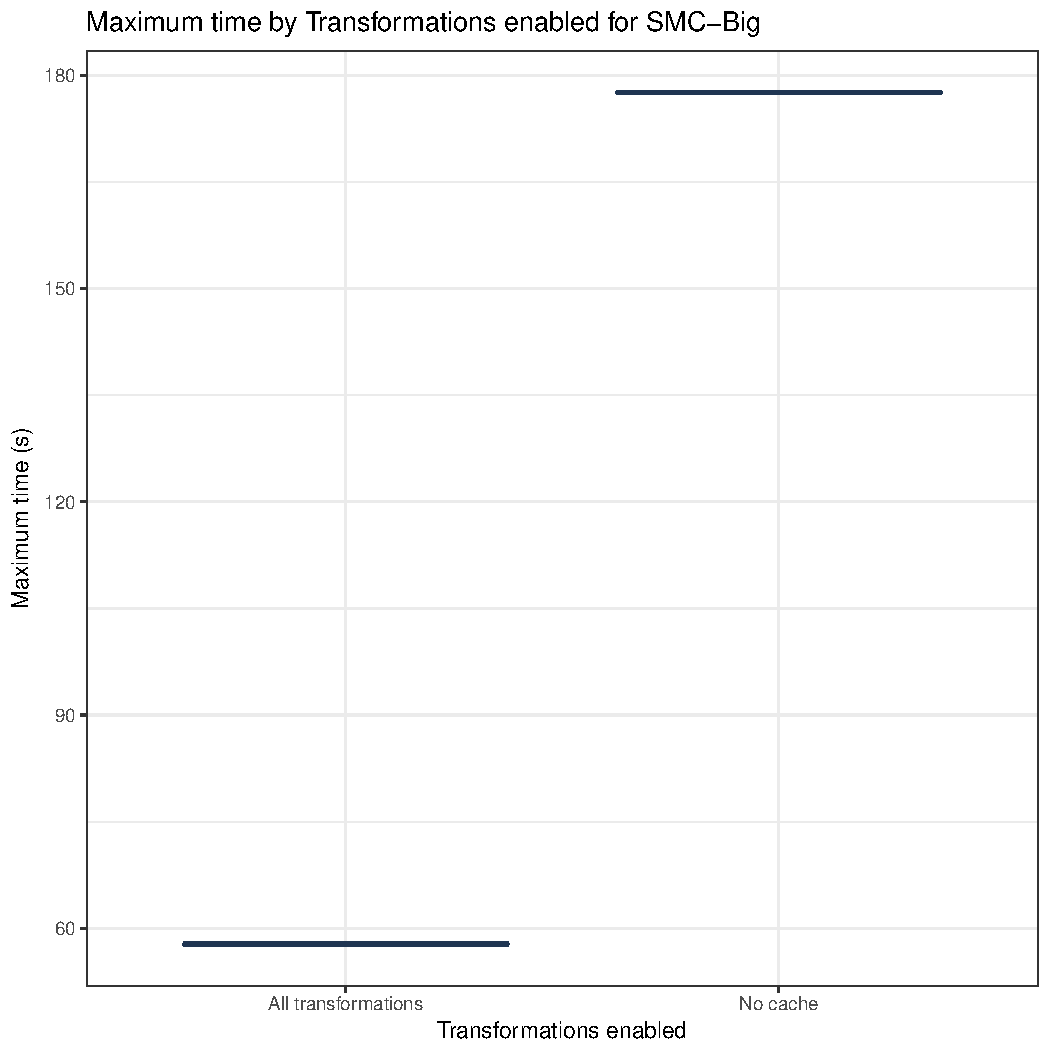
\includegraphics[width=\maxwidth]{figure/RH2_big-1} 
\begin{kframe}

{\ttfamily\noindent\bfseries\color{errorcolor}{\#\# Error in eval(expr, envir, enclos): object 'shap\_cashew\_big' not found}}\begin{verbatim}
## [1] ""
## [1] "Means comparison"
## [1] "Mean Maximum time for All transformations:  57.7936"
## [1] "Mean Maximum time for No cache:  177.562"
## [1] "Absolute difference:  119.7684"
## Maximum time for No cache is  207.234711109881 % greater than 
## Maximum time for All transformations
\end{verbatim}
\end{kframe}
\end{knitrout}


 

	
	\subsubsection{RH2 Results: Maximum time All transformations = No cache}
	
	
	\begin{table}[H]
	\centering
	\caption{RH2 Results per Object}
	\begin{tabular}{ll}
	\textbf{SMC-Small} & Inconclusive \\
	\textbf{SMC-Big} & Inconclusive \\
	\end{tabular}
	\end{table}

	\begin{table}[H]
	\centering
	\caption{RH2 Results Summary}
	\begin{tabular}{ll}
	\textbf{All transformations \textless{} No cache:}& 0\% \\
	\textbf{All transformations \textgreater{} No cache:}& 0\%\\
	\textbf{All transformations:} & 0\%\\
	\textbf{No cache:} & 0\%\\
	\textbf{None:}& 0\%\\
	\textbf{Inconclusive:}& 100\%
			
	
	\end{tabular}
	\end{table}
	
	
	



\subsection{RH3: Total time for Cashew is equals than Average time for No Cache}


 
\begin{knitrout}
\definecolor{shadecolor}{rgb}{0.969, 0.969, 0.969}\color{fgcolor}
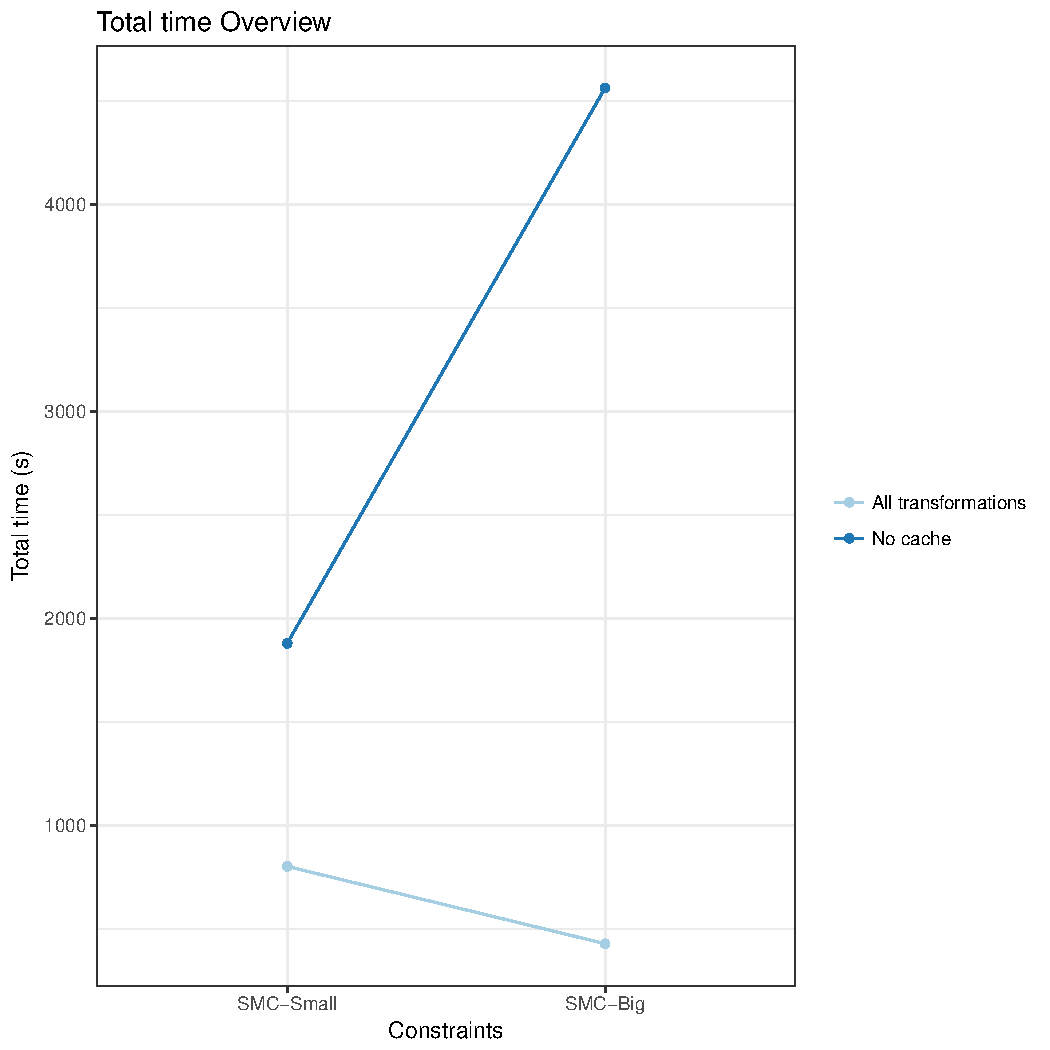
\includegraphics[width=\maxwidth]{figure/overview_RH3-1} 

\end{knitrout}
 	

\subsubsection{RH3.1: Object SMC-Small}

 \textbf{Total time for All transformations}
\begin{knitrout}
\definecolor{shadecolor}{rgb}{0.969, 0.969, 0.969}\color{fgcolor}\begin{kframe}
\begin{verbatim}
## [1] "Sample size:  1"
##    Min. 1st Qu.  Median    Mean 3rd Qu.    Max. 
##   803.8   803.8   803.8   803.8   803.8   803.8
\end{verbatim}


{\ttfamily\noindent\bfseries\color{errorcolor}{\#\# Error in shapiro.test(subset(json\_data, treatment == "{}cashew"{} \& object == : sample size must be between 3 and 5000}}\end{kframe}
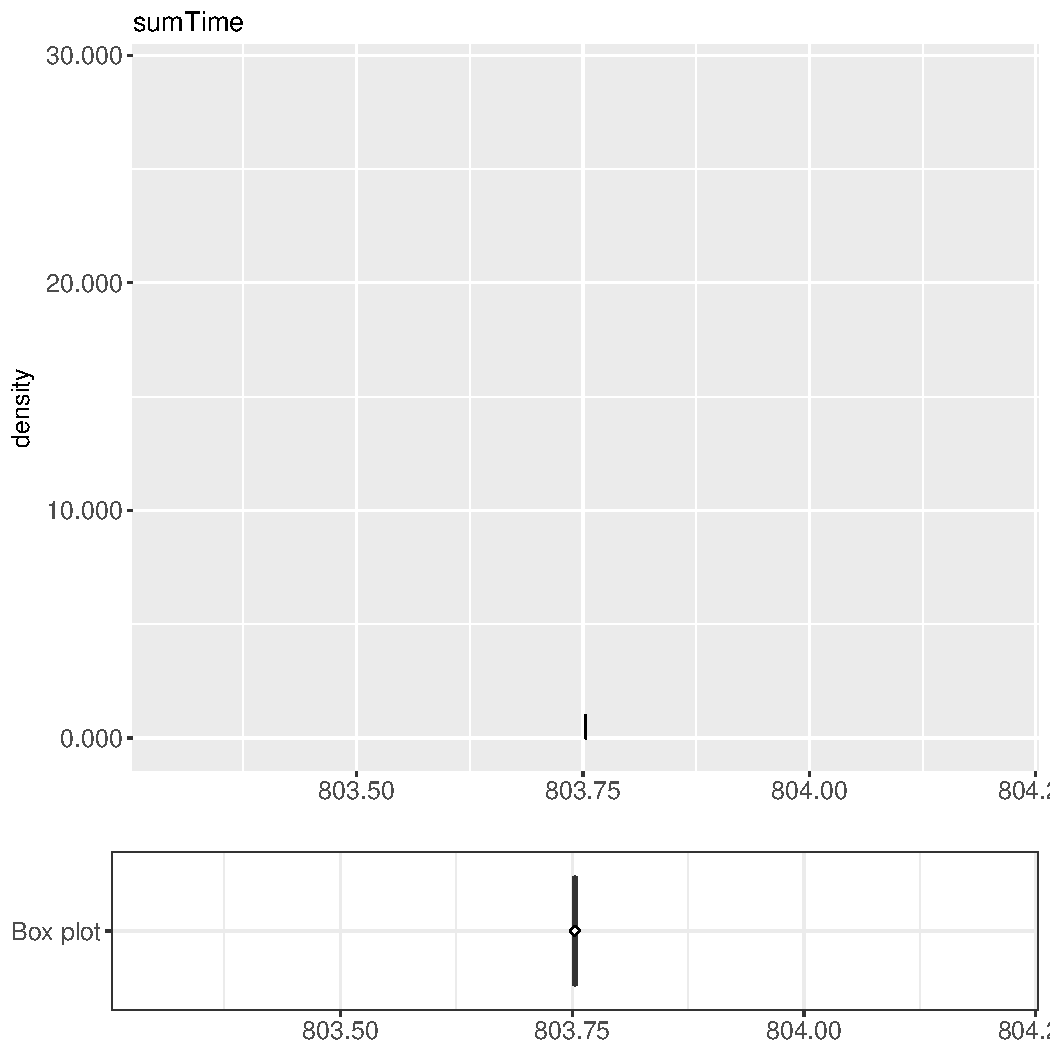
\includegraphics[width=\maxwidth]{figure/RH3_cashew_small-1} 

\end{knitrout}
 \textbf{Total time for No cache}
\begin{knitrout}
\definecolor{shadecolor}{rgb}{0.969, 0.969, 0.969}\color{fgcolor}\begin{kframe}
\begin{verbatim}
## [1] "Sample size:  1"
##    Min. 1st Qu.  Median    Mean 3rd Qu.    Max. 
##    1880    1880    1880    1880    1880    1880
\end{verbatim}


{\ttfamily\noindent\bfseries\color{errorcolor}{\#\# Error in shapiro.test(subset(json\_data, treatment == "{}noCache"{} \& object == : sample size must be between 3 and 5000}}\end{kframe}
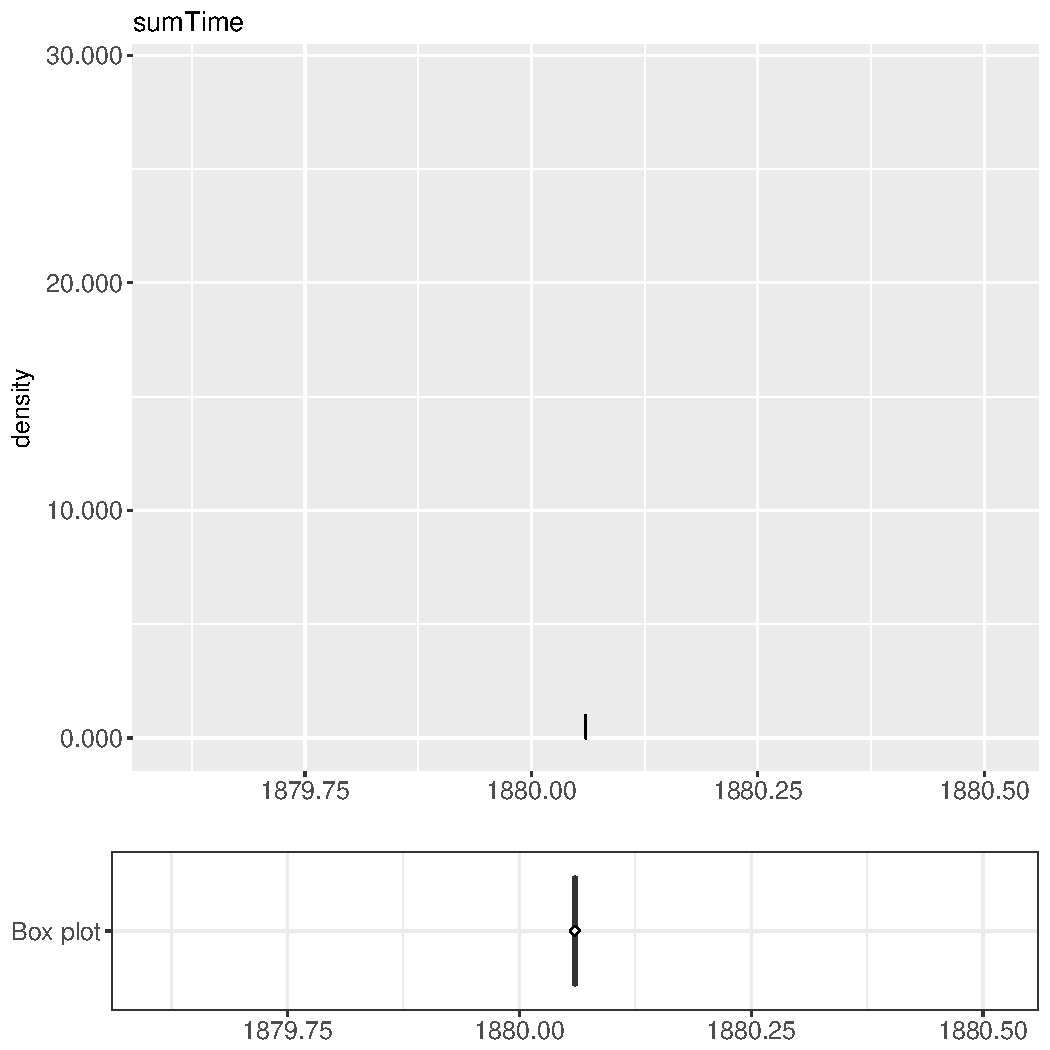
\includegraphics[width=\maxwidth]{figure/RH3_noCache_small-1} 

\end{knitrout}
  
 \textbf{Comparison}
  
\begin{knitrout}
\definecolor{shadecolor}{rgb}{0.969, 0.969, 0.969}\color{fgcolor}
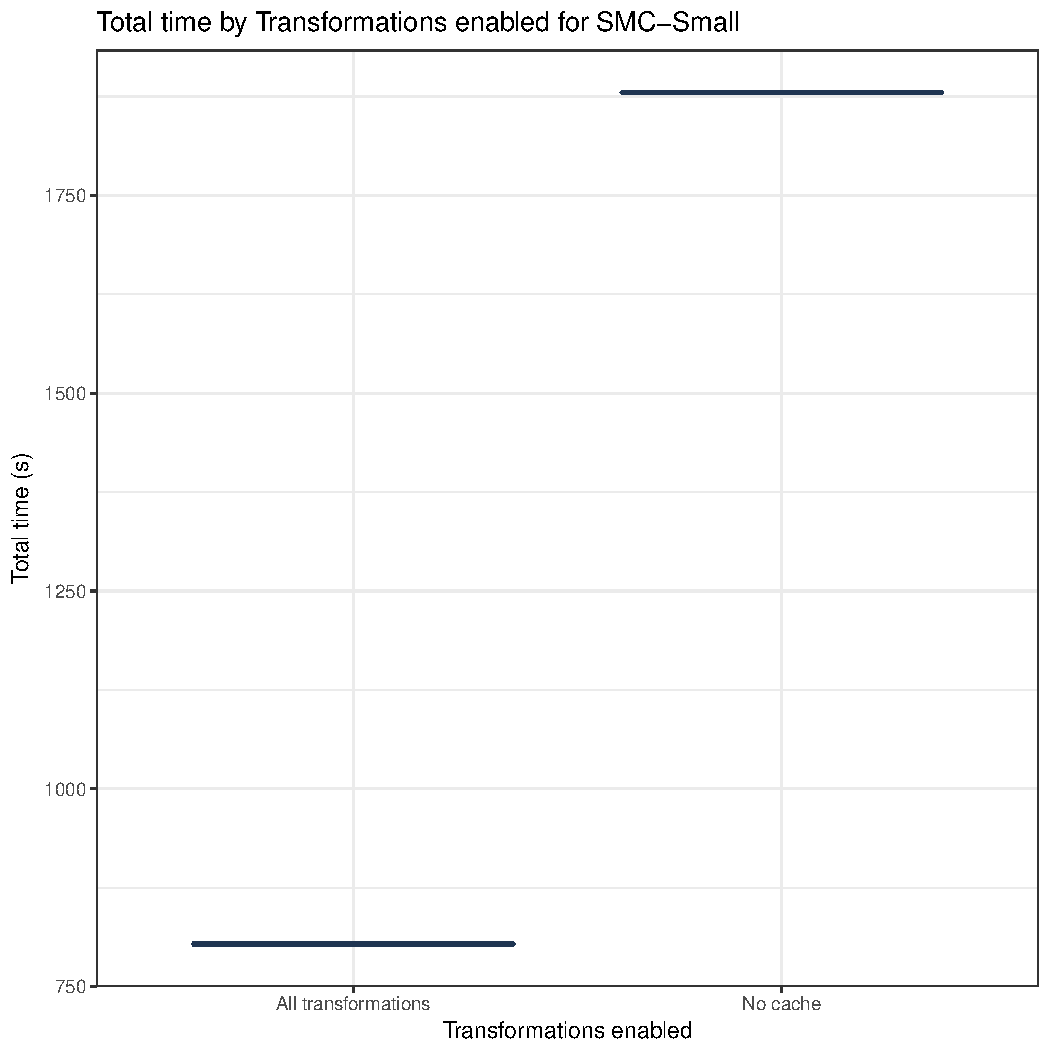
\includegraphics[width=\maxwidth]{figure/RH3_small-1} 
\begin{kframe}

{\ttfamily\noindent\bfseries\color{errorcolor}{\#\# Error in eval(expr, envir, enclos): object 'shap\_cashew\_small' not found}}\begin{verbatim}
## [1] ""
## [1] "Means comparison"
## [1] "Mean Total time for All transformations:  803.753"
## [1] "Mean Total time for No cache:  1880.06"
## [1] "Absolute difference:  1076.307"
## Total time for No cache is  133.910168920054 % greater than 
## Total time for All transformations
\end{verbatim}
\end{kframe}
\end{knitrout}


\subsubsection{RH3.2: Object SMC-Big}

 \textbf{Total time for All transformations}
\begin{knitrout}
\definecolor{shadecolor}{rgb}{0.969, 0.969, 0.969}\color{fgcolor}\begin{kframe}
\begin{verbatim}
## [1] "Sample size:  1"
##    Min. 1st Qu.  Median    Mean 3rd Qu.    Max. 
##   430.5   430.5   430.5   430.5   430.5   430.5
\end{verbatim}


{\ttfamily\noindent\bfseries\color{errorcolor}{\#\# Error in shapiro.test(subset(json\_data, treatment == "{}cashew"{} \& object == : sample size must be between 3 and 5000}}\end{kframe}
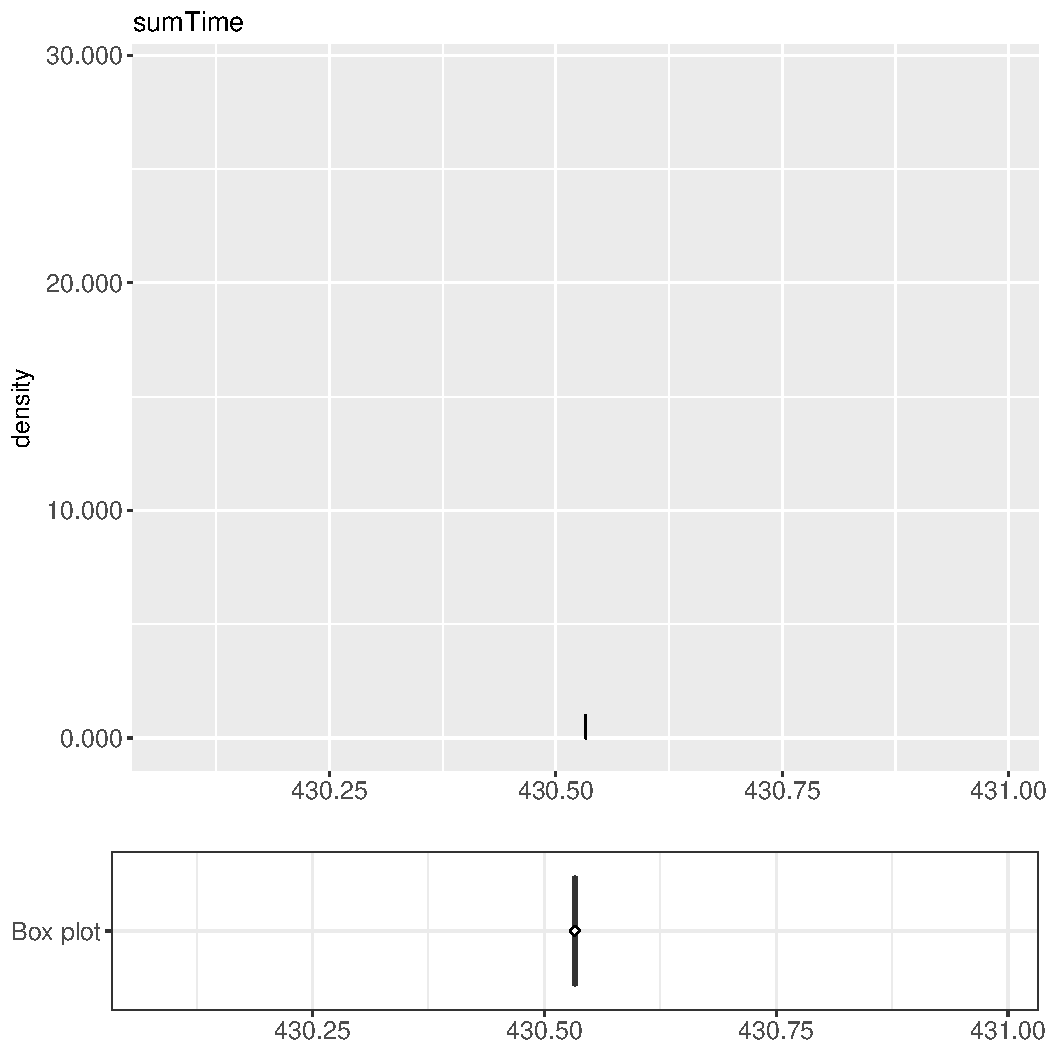
\includegraphics[width=\maxwidth]{figure/RH3_cashew_big-1} 

\end{knitrout}
 \textbf{Total time for No cache}
\begin{knitrout}
\definecolor{shadecolor}{rgb}{0.969, 0.969, 0.969}\color{fgcolor}\begin{kframe}
\begin{verbatim}
## [1] "Sample size:  1"
##    Min. 1st Qu.  Median    Mean 3rd Qu.    Max. 
##    4562    4562    4562    4562    4562    4562
\end{verbatim}


{\ttfamily\noindent\bfseries\color{errorcolor}{\#\# Error in shapiro.test(subset(json\_data, treatment == "{}noCache"{} \& object == : sample size must be between 3 and 5000}}\end{kframe}
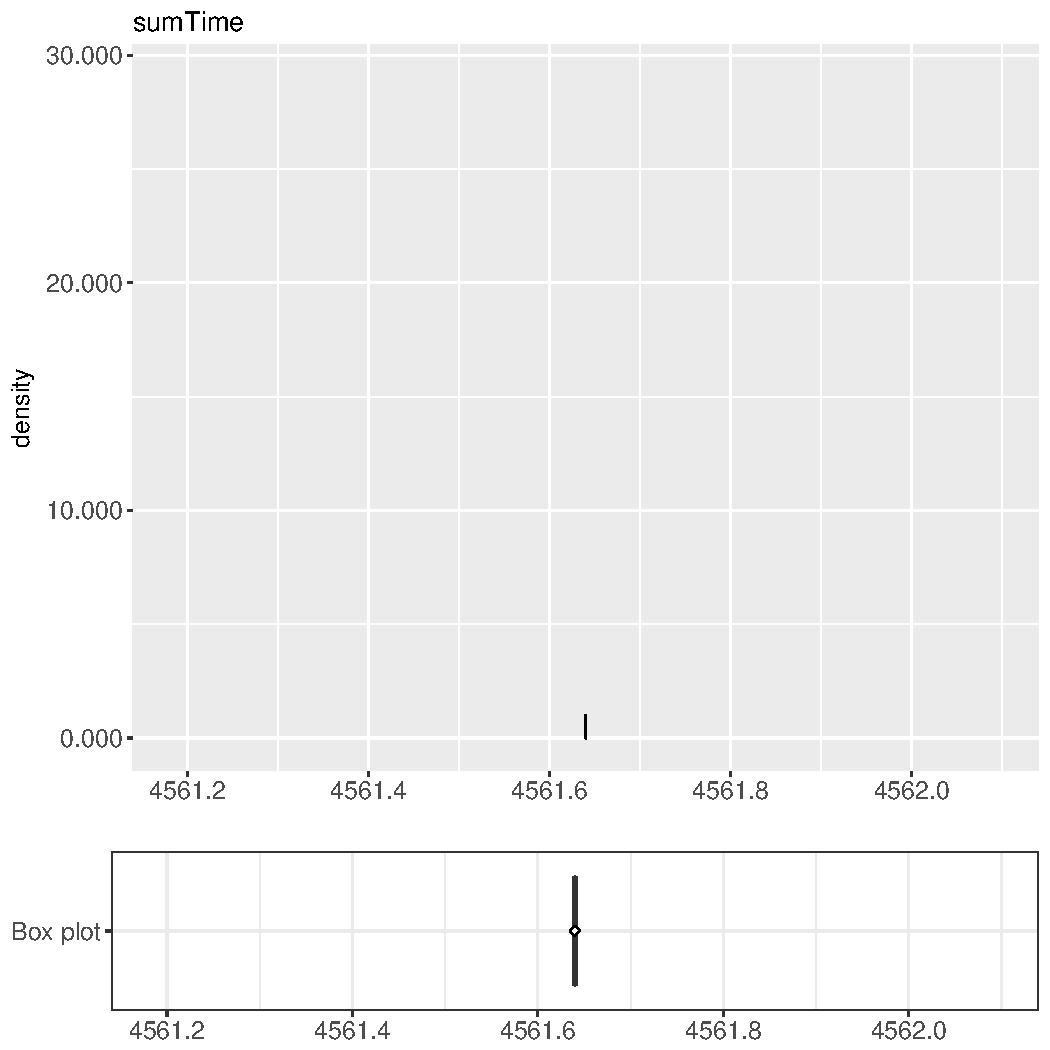
\includegraphics[width=\maxwidth]{figure/RH3_noCache_big-1} 

\end{knitrout}
  
 \textbf{Comparison}
  
\begin{knitrout}
\definecolor{shadecolor}{rgb}{0.969, 0.969, 0.969}\color{fgcolor}
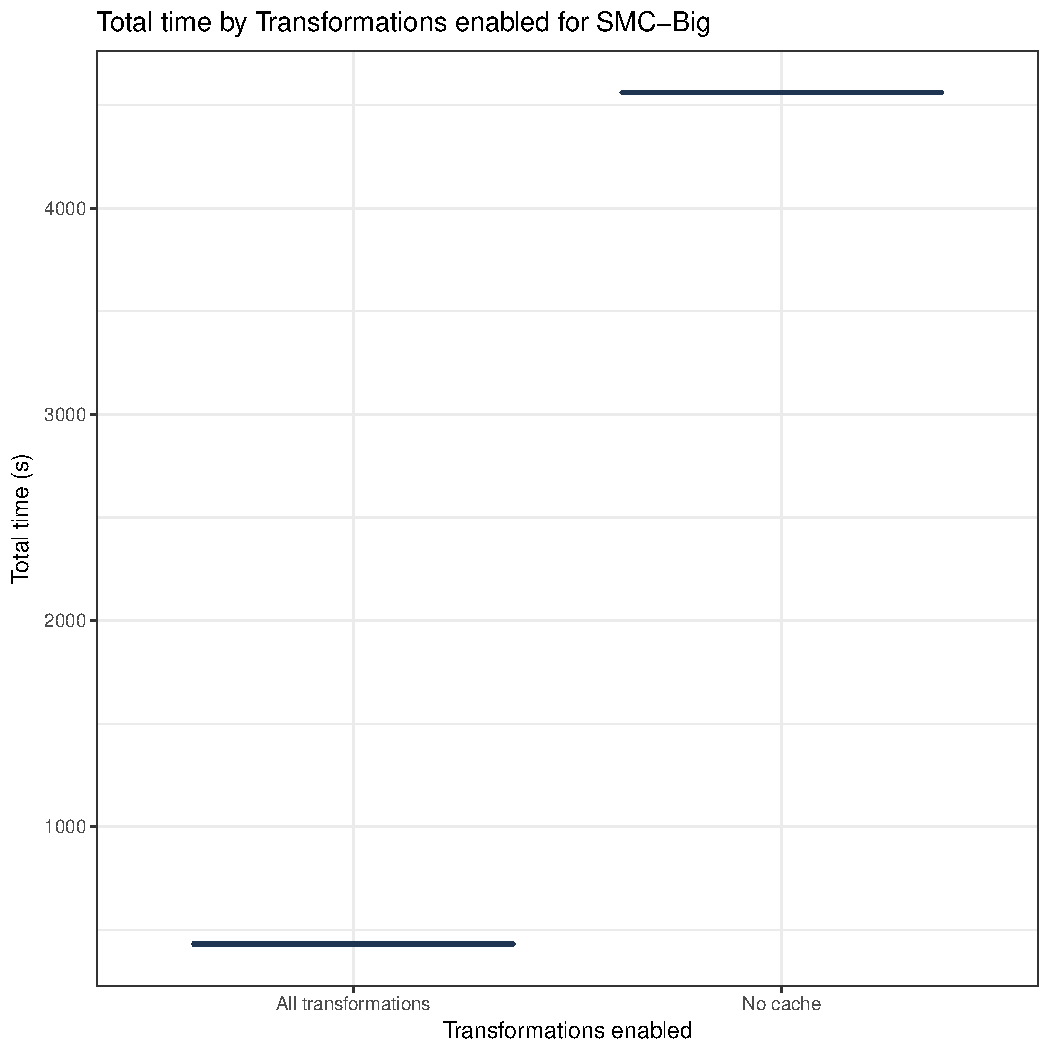
\includegraphics[width=\maxwidth]{figure/RH3_big-1} 
\begin{kframe}

{\ttfamily\noindent\bfseries\color{errorcolor}{\#\# Error in eval(expr, envir, enclos): object 'shap\_cashew\_big' not found}}\begin{verbatim}
## [1] ""
## [1] "Means comparison"
## [1] "Mean Total time for All transformations:  430.533"
## [1] "Mean Total time for No cache:  4561.64"
## [1] "Absolute difference:  4131.107"
## Total time for No cache is  959.533183286763 % greater than 
## Total time for All transformations
\end{verbatim}
\end{kframe}
\end{knitrout}


 

	
	\subsubsection{RH3 Results: Total time All transformations = No cache}
	
	
	\begin{table}[H]
	\centering
	\caption{RH3 Results per Object}
	\begin{tabular}{ll}
	\textbf{SMC-Small} & Inconclusive \\
	\textbf{SMC-Big} & Inconclusive \\
	\end{tabular}
	\end{table}

	\begin{table}[H]
	\centering
	\caption{RH3 Results Summary}
	\begin{tabular}{ll}
	\textbf{All transformations \textless{} No cache:}& 0\% \\
	\textbf{All transformations \textgreater{} No cache:}& 0\%\\
	\textbf{All transformations:} & 0\%\\
	\textbf{No cache:} & 0\%\\
	\textbf{None:}& 0\%\\
	\textbf{Inconclusive:}& 100\%
			
	
	\end{tabular}
	\end{table}
	
	
	



\subsection{RH4: Number of Orbits for Cashew is equals than the Number of Orbits for No Cache}


 
\begin{knitrout}
\definecolor{shadecolor}{rgb}{0.969, 0.969, 0.969}\color{fgcolor}
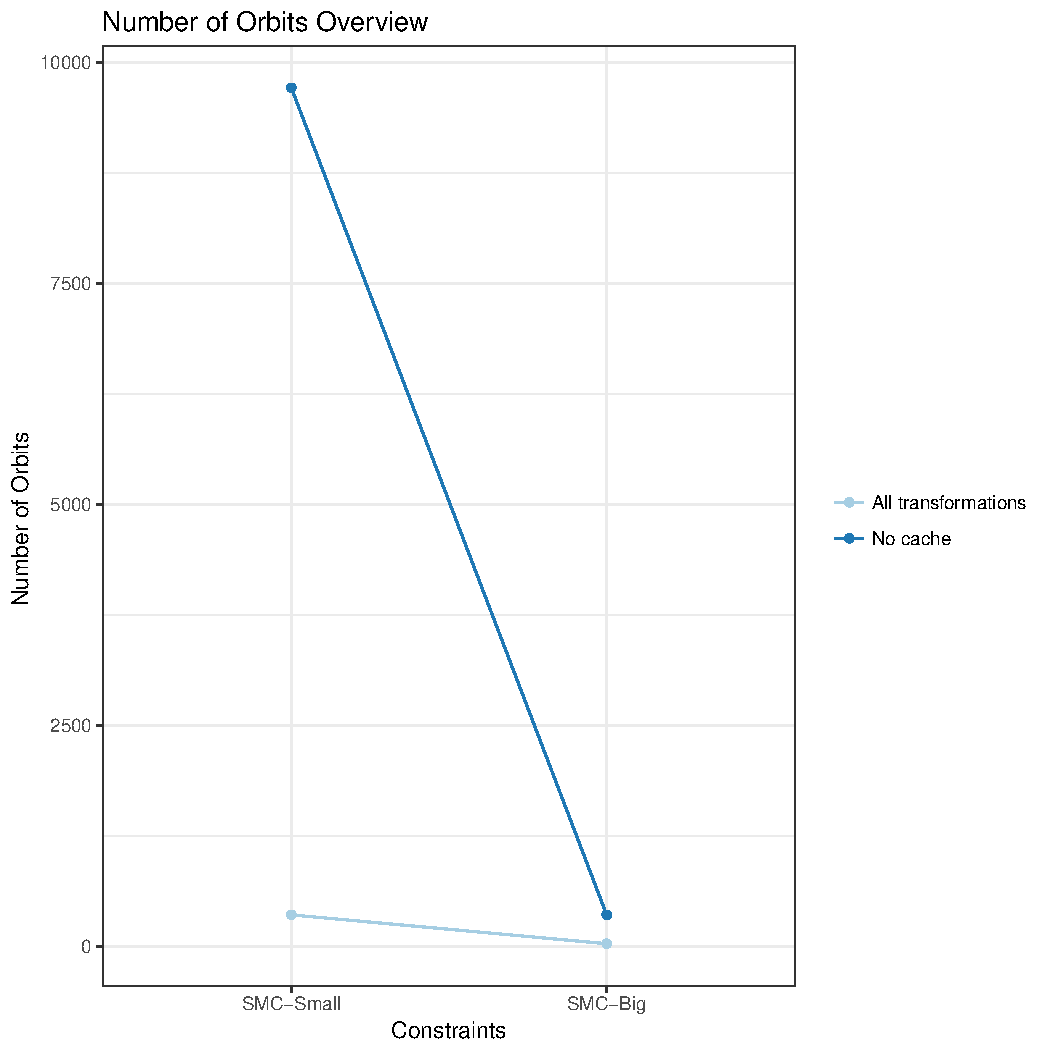
\includegraphics[width=\maxwidth]{figure/overview_RH4-1} 

\end{knitrout}
 	

\subsubsection{RH4.1: Object SMC-Small}

 \textbf{Number of Orbits for All transformations}
\begin{knitrout}
\definecolor{shadecolor}{rgb}{0.969, 0.969, 0.969}\color{fgcolor}\begin{kframe}
\begin{verbatim}
## [1] "Sample size:  1"
##    Min. 1st Qu.  Median    Mean 3rd Qu.    Max. 
##     360     360     360     360     360     360
\end{verbatim}


{\ttfamily\noindent\bfseries\color{errorcolor}{\#\# Error in shapiro.test(subset(json\_data, treatment == "{}cashew"{} \& object == : sample size must be between 3 and 5000}}\end{kframe}
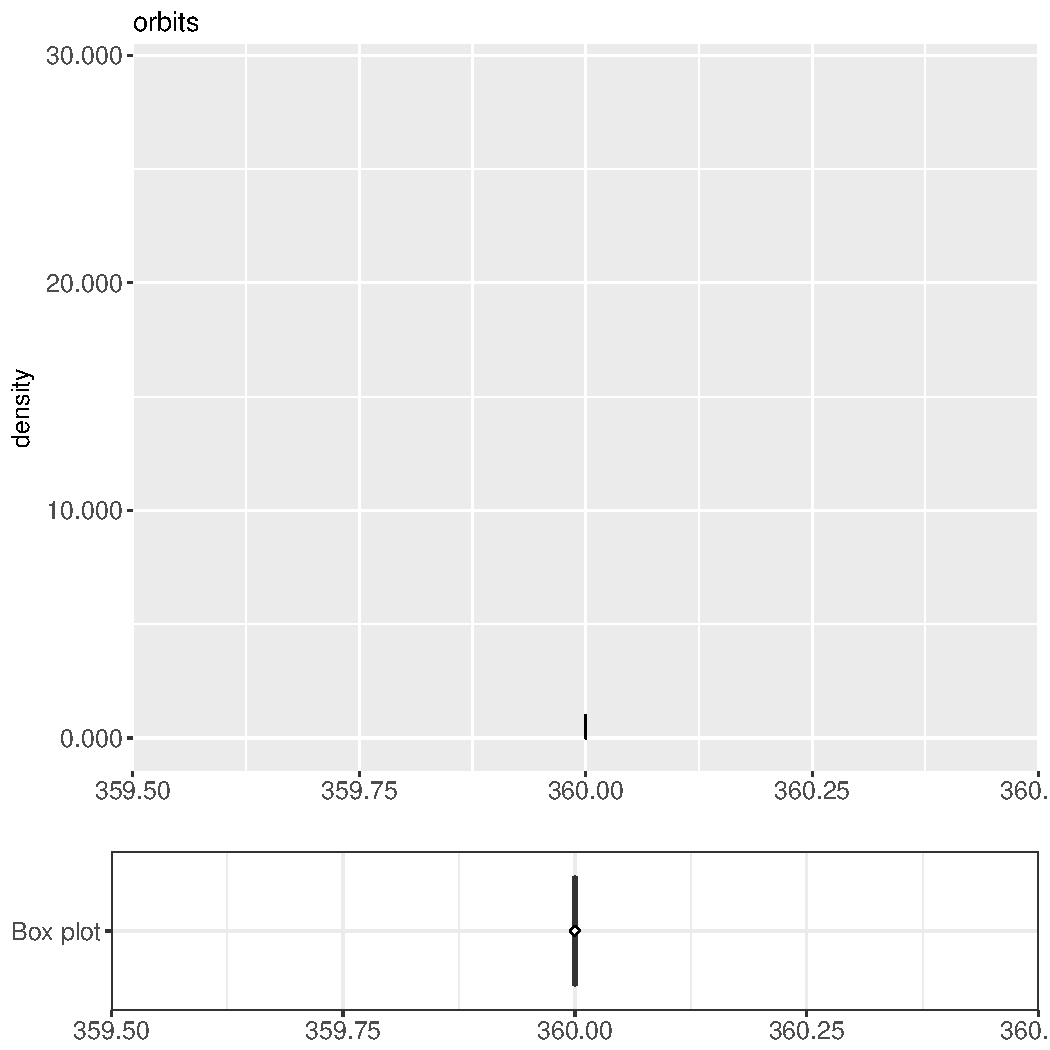
\includegraphics[width=\maxwidth]{figure/RH4_cashew_small-1} 

\end{knitrout}
 \textbf{Number of Orbits for No cache}
\begin{knitrout}
\definecolor{shadecolor}{rgb}{0.969, 0.969, 0.969}\color{fgcolor}\begin{kframe}
\begin{verbatim}
## [1] "Sample size:  1"
##    Min. 1st Qu.  Median    Mean 3rd Qu.    Max. 
##    9710    9710    9710    9710    9710    9710
\end{verbatim}


{\ttfamily\noindent\bfseries\color{errorcolor}{\#\# Error in shapiro.test(subset(json\_data, treatment == "{}noCache"{} \& object == : sample size must be between 3 and 5000}}\end{kframe}
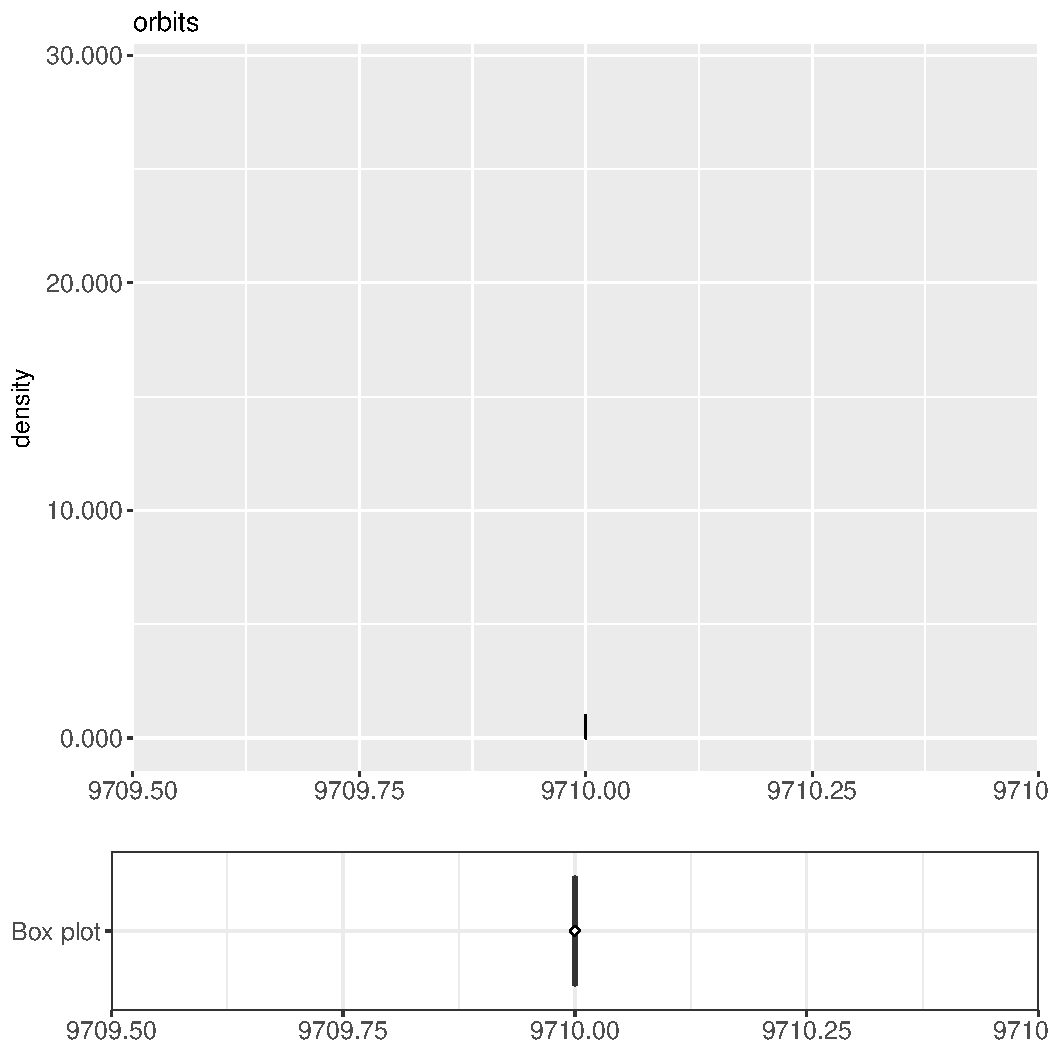
\includegraphics[width=\maxwidth]{figure/RH4_noCache_small-1} 

\end{knitrout}
  
 \textbf{Comparison}
  
\begin{knitrout}
\definecolor{shadecolor}{rgb}{0.969, 0.969, 0.969}\color{fgcolor}
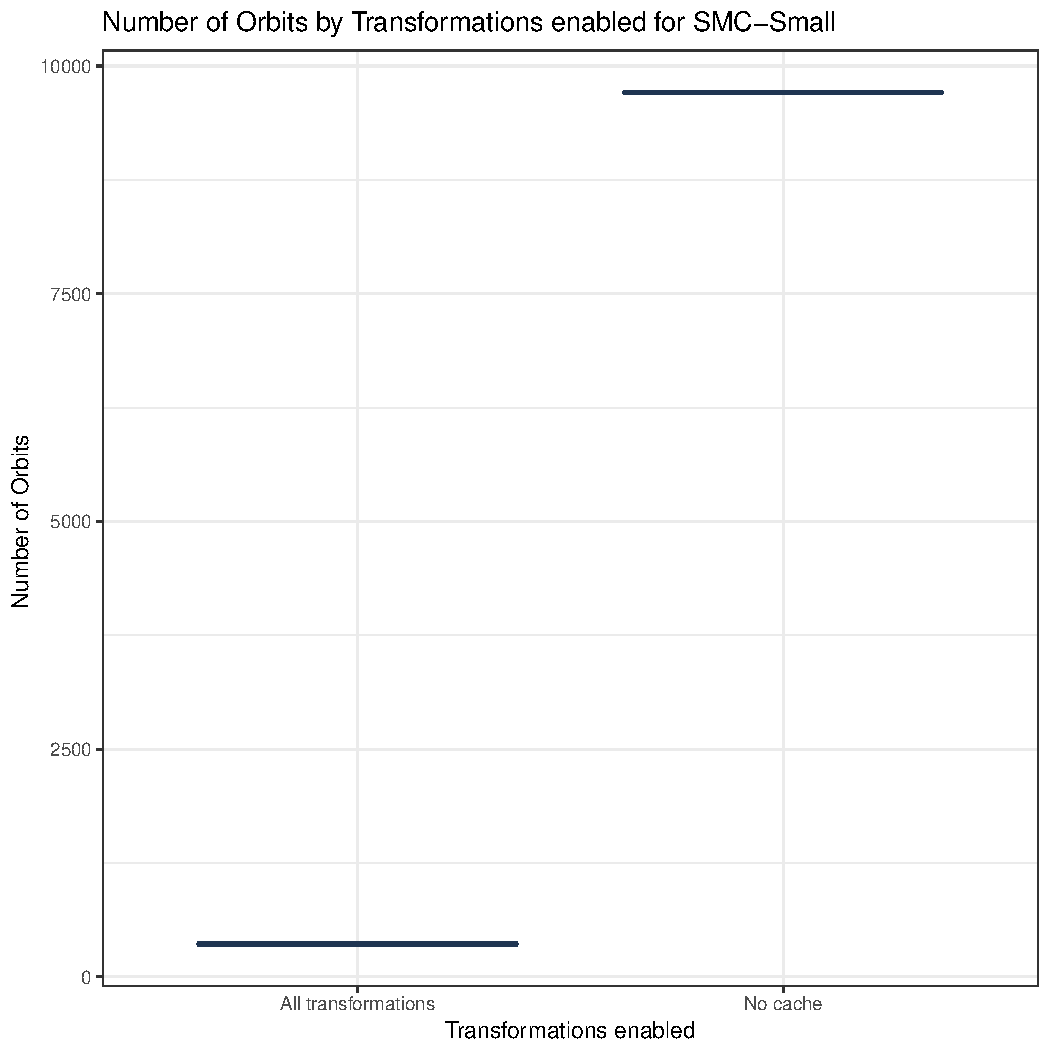
\includegraphics[width=\maxwidth]{figure/RH4_small-1} 
\begin{kframe}

{\ttfamily\noindent\bfseries\color{errorcolor}{\#\# Error in eval(expr, envir, enclos): object 'shap\_cashew\_small' not found}}\begin{verbatim}
## [1] ""
## [1] "Means comparison"
## [1] "Mean Number of Orbits for All transformations:  360"
## [1] "Mean Number of Orbits for No cache:  9710"
## [1] "Absolute difference:  9350"
## Number of Orbits for No cache is  2597.22222222222 % greater than 
## Number of Orbits for All transformations
\end{verbatim}
\end{kframe}
\end{knitrout}


\subsubsection{RH4.2: Object SMC-Big}

 \textbf{Number of Orbits for All transformations}
\begin{knitrout}
\definecolor{shadecolor}{rgb}{0.969, 0.969, 0.969}\color{fgcolor}\begin{kframe}
\begin{verbatim}
## [1] "Sample size:  1"
##    Min. 1st Qu.  Median    Mean 3rd Qu.    Max. 
##      34      34      34      34      34      34
\end{verbatim}


{\ttfamily\noindent\bfseries\color{errorcolor}{\#\# Error in shapiro.test(subset(json\_data, treatment == "{}cashew"{} \& object == : sample size must be between 3 and 5000}}\end{kframe}
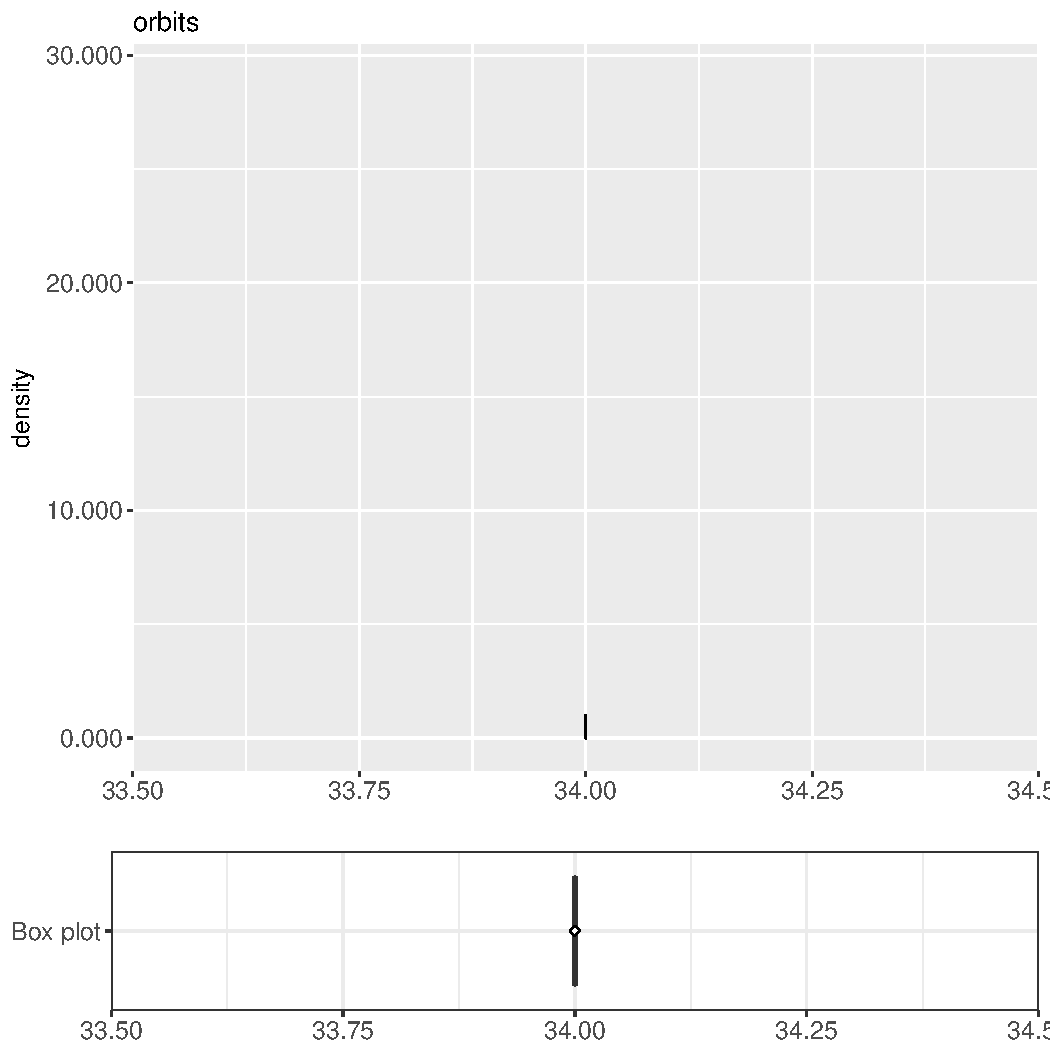
\includegraphics[width=\maxwidth]{figure/RH4_cashew_big-1} 

\end{knitrout}
 \textbf{Number of Orbits for No cache}
\begin{knitrout}
\definecolor{shadecolor}{rgb}{0.969, 0.969, 0.969}\color{fgcolor}\begin{kframe}
\begin{verbatim}
## [1] "Sample size:  1"
##    Min. 1st Qu.  Median    Mean 3rd Qu.    Max. 
##     359     359     359     359     359     359
\end{verbatim}


{\ttfamily\noindent\bfseries\color{errorcolor}{\#\# Error in shapiro.test(subset(json\_data, treatment == "{}noCache"{} \& object == : sample size must be between 3 and 5000}}\end{kframe}
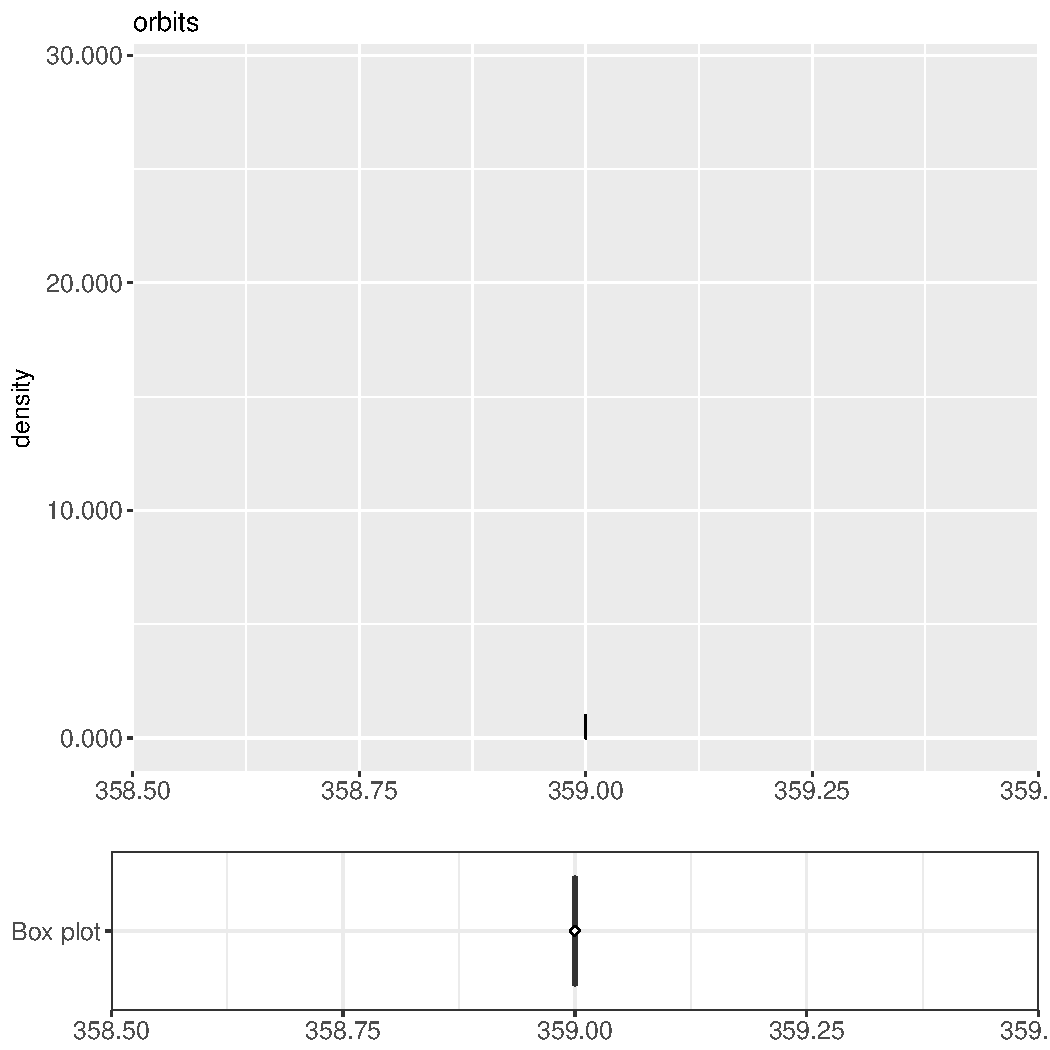
\includegraphics[width=\maxwidth]{figure/RH4_noCache_big-1} 

\end{knitrout}
  
 \textbf{Comparison}
  
\begin{knitrout}
\definecolor{shadecolor}{rgb}{0.969, 0.969, 0.969}\color{fgcolor}
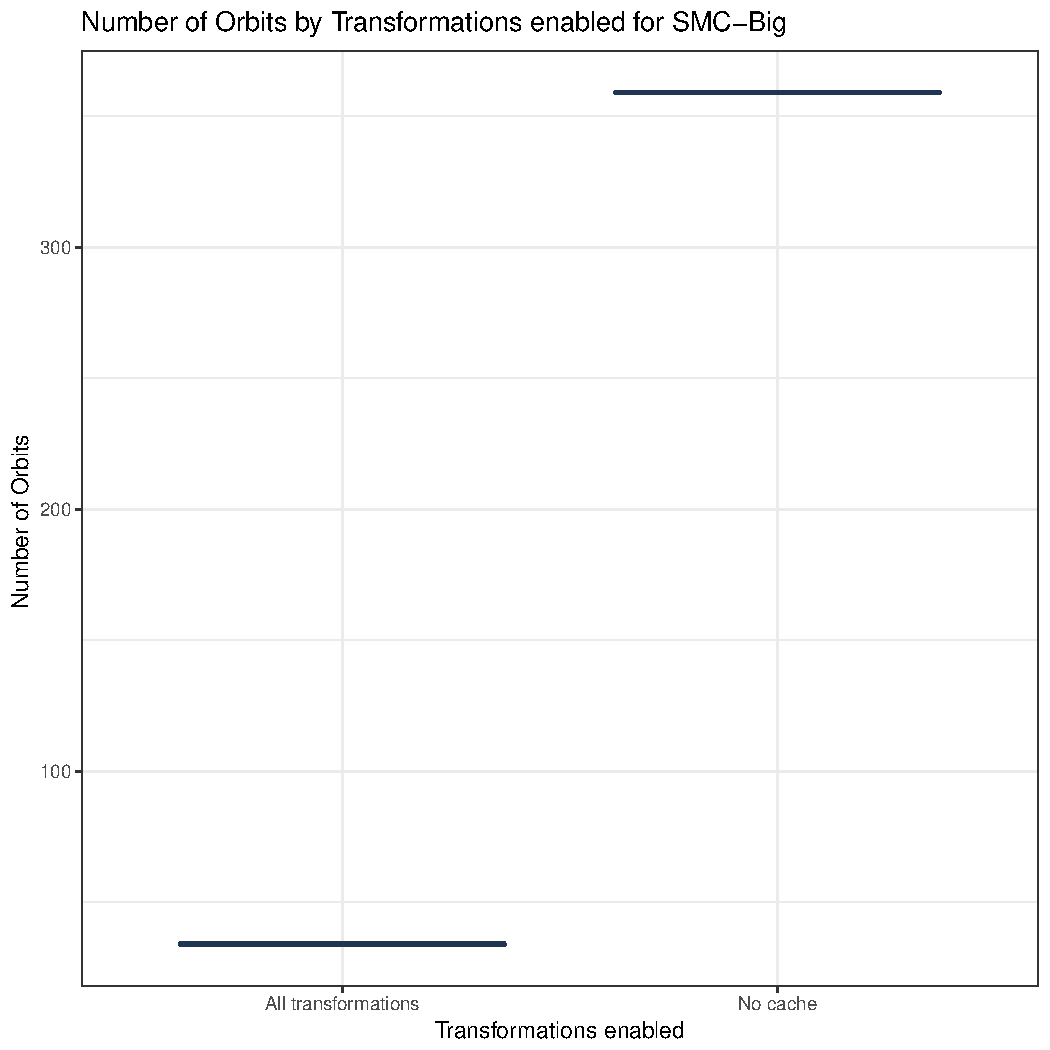
\includegraphics[width=\maxwidth]{figure/RH4_big-1} 
\begin{kframe}

{\ttfamily\noindent\bfseries\color{errorcolor}{\#\# Error in eval(expr, envir, enclos): object 'shap\_cashew\_big' not found}}\begin{verbatim}
## [1] ""
## [1] "Means comparison"
## [1] "Mean Number of Orbits for All transformations:  34"
## [1] "Mean Number of Orbits for No cache:  359"
## [1] "Absolute difference:  325"
## Number of Orbits for No cache is  955.882352941176 % greater than 
## Number of Orbits for All transformations
\end{verbatim}
\end{kframe}
\end{knitrout}


 

	
	\subsubsection{RH4 Results: Number of Orbits All transformations = No cache}
	
	
	\begin{table}[H]
	\centering
	\caption{RH4 Results per Object}
	\begin{tabular}{ll}
	\textbf{SMC-Small} & Inconclusive \\
	\textbf{SMC-Big} & Inconclusive \\
	\end{tabular}
	\end{table}

	\begin{table}[H]
	\centering
	\caption{RH4 Results Summary}
	\begin{tabular}{ll}
	\textbf{All transformations \textless{} No cache:}& 0\% \\
	\textbf{All transformations \textgreater{} No cache:}& 0\%\\
	\textbf{All transformations:} & 0\%\\
	\textbf{No cache:} & 0\%\\
	\textbf{None:}& 0\%\\
	\textbf{Inconclusive:}& 100\%
			
	
	\end{tabular}
	\end{table}
	
	
	



\subsection{RH5: Number of Orbits for Cashew is equals than the Number of Orbits for Cashew Except Order}


 
\begin{knitrout}
\definecolor{shadecolor}{rgb}{0.969, 0.969, 0.969}\color{fgcolor}
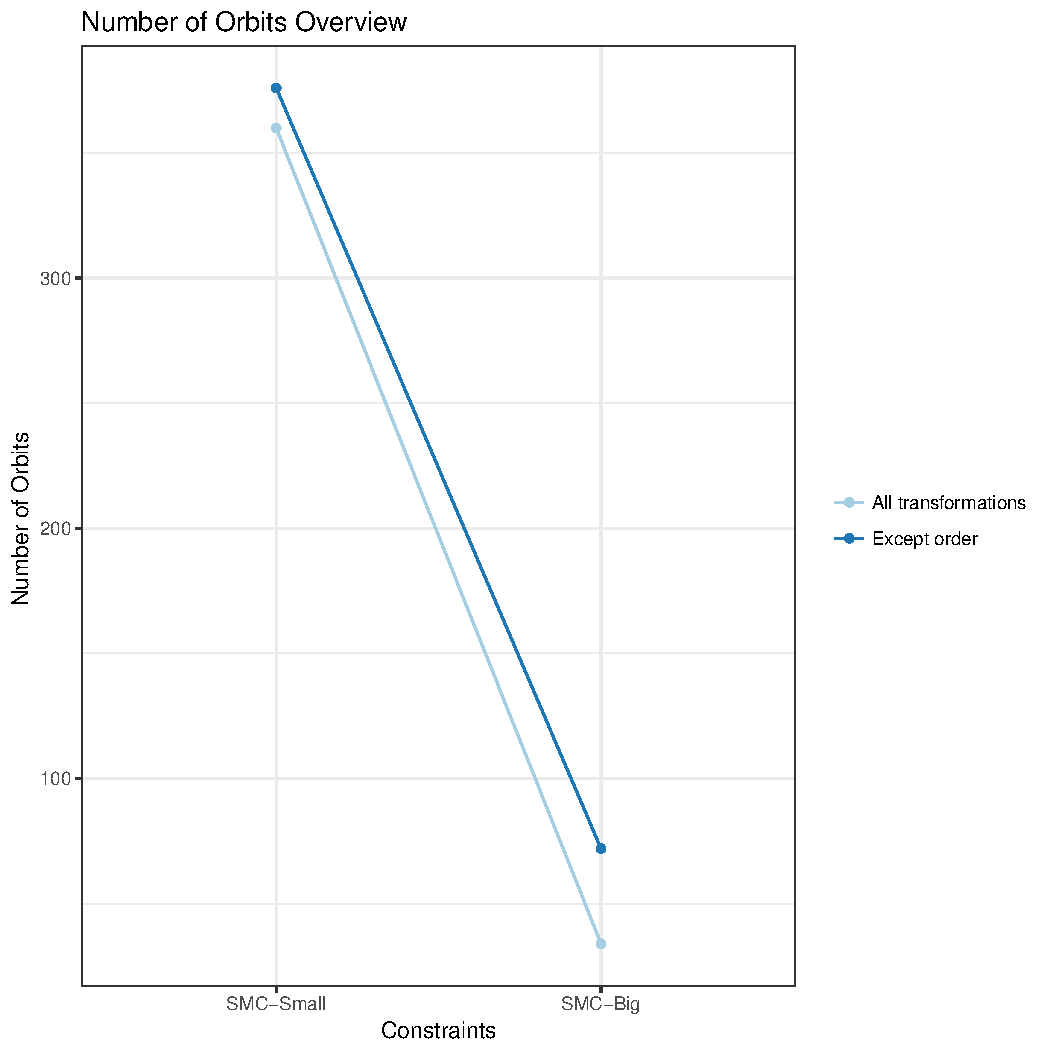
\includegraphics[width=\maxwidth]{figure/overview_RH5-1} 

\end{knitrout}
 	

\subsubsection{RH5.1: Object SMC-Small}

 \textbf{Number of Orbits for All transformations}
\begin{knitrout}
\definecolor{shadecolor}{rgb}{0.969, 0.969, 0.969}\color{fgcolor}\begin{kframe}
\begin{verbatim}
## [1] "Sample size:  1"
##    Min. 1st Qu.  Median    Mean 3rd Qu.    Max. 
##     360     360     360     360     360     360
\end{verbatim}


{\ttfamily\noindent\bfseries\color{errorcolor}{\#\# Error in shapiro.test(subset(json\_data, treatment == "{}cashew"{} \& object == : sample size must be between 3 and 5000}}\end{kframe}
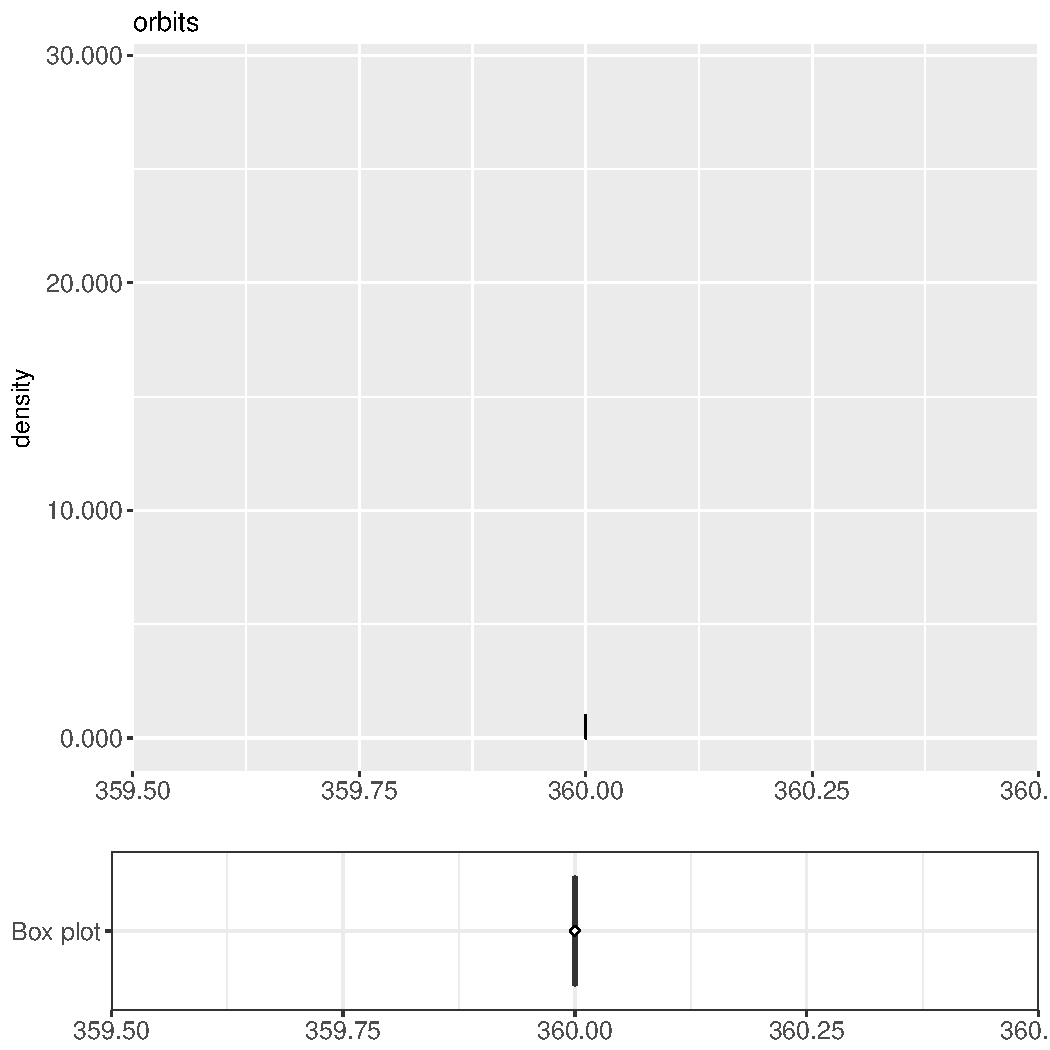
\includegraphics[width=\maxwidth]{figure/RH5_cashew_small-1} 

\end{knitrout}
 \textbf{Number of Orbits for Except order}
\begin{knitrout}
\definecolor{shadecolor}{rgb}{0.969, 0.969, 0.969}\color{fgcolor}\begin{kframe}
\begin{verbatim}
## [1] "Sample size:  1"
##    Min. 1st Qu.  Median    Mean 3rd Qu.    Max. 
##     376     376     376     376     376     376
\end{verbatim}


{\ttfamily\noindent\bfseries\color{errorcolor}{\#\# Error in shapiro.test(subset(json\_data, treatment == "{}cashewExceptOrder"{} \& : sample size must be between 3 and 5000}}\end{kframe}
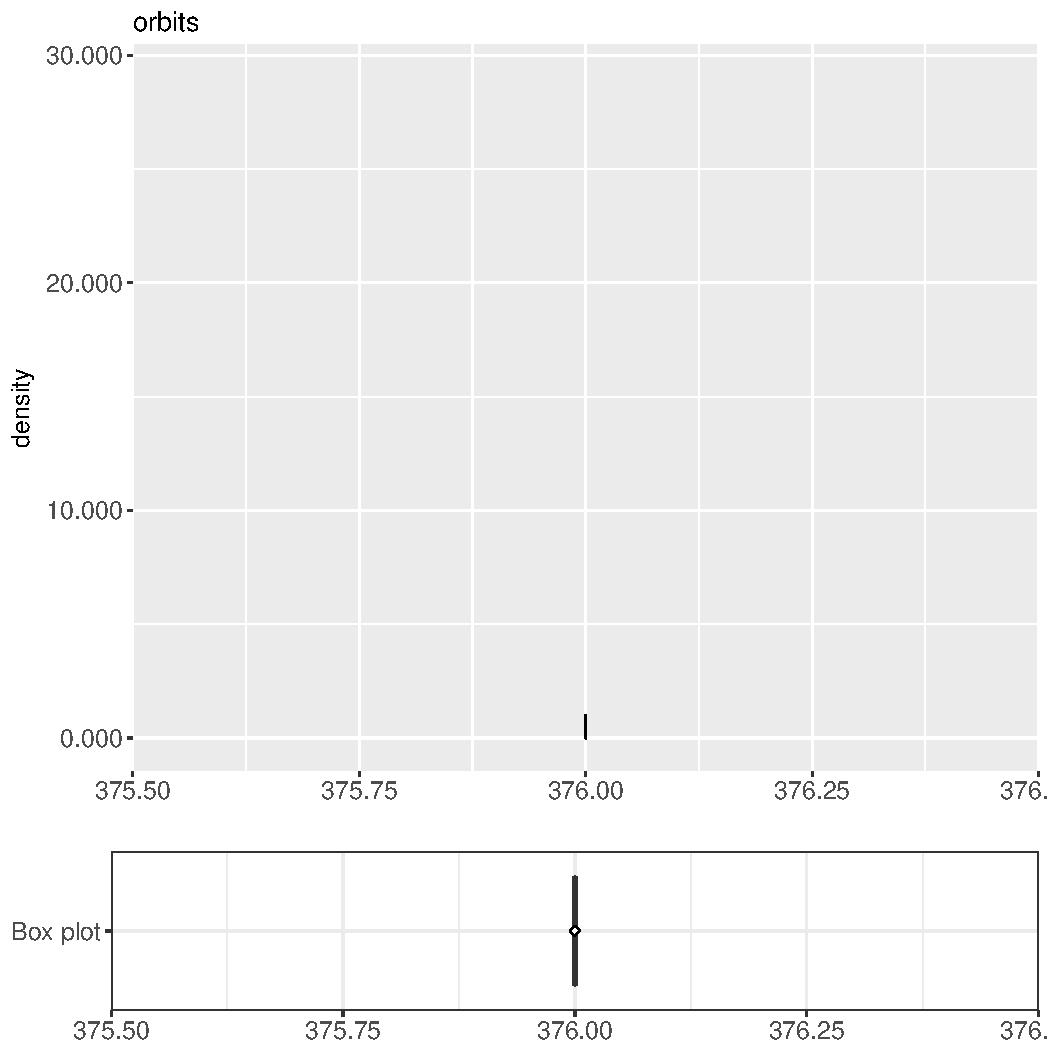
\includegraphics[width=\maxwidth]{figure/RH5_cashewExceptOrder_small-1} 

\end{knitrout}
  
 \textbf{Comparison}
  
\begin{knitrout}
\definecolor{shadecolor}{rgb}{0.969, 0.969, 0.969}\color{fgcolor}
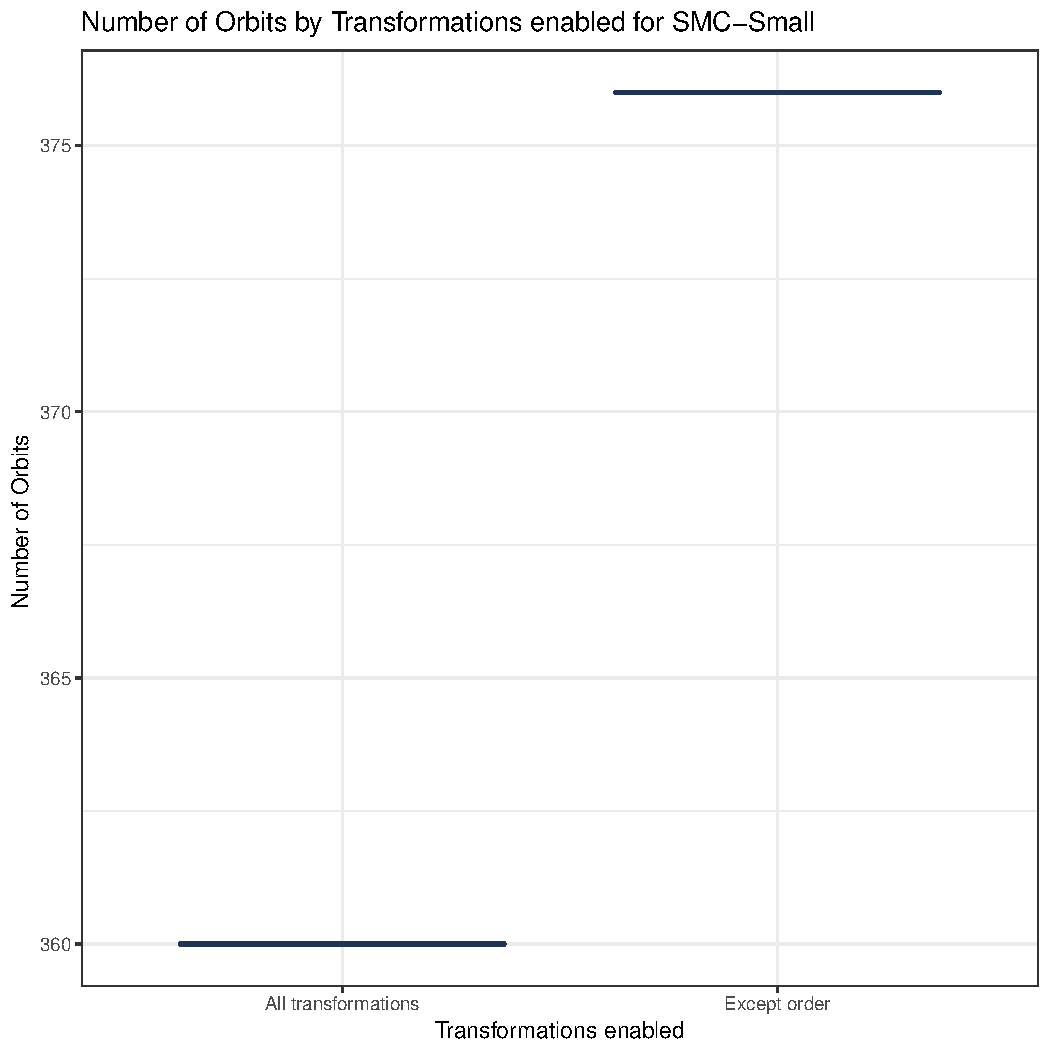
\includegraphics[width=\maxwidth]{figure/RH5_small-1} 
\begin{kframe}

{\ttfamily\noindent\bfseries\color{errorcolor}{\#\# Error in eval(expr, envir, enclos): object 'shap\_cashew\_small' not found}}\begin{verbatim}
## [1] ""
## [1] "Means comparison"
## [1] "Mean Number of Orbits for All transformations:  360"
## [1] "Mean Number of Orbits for Except order:  376"
## [1] "Absolute difference:  16"
## Number of Orbits for Except order is  4.44444444444444 % greater than 
## Number of Orbits for All transformations
\end{verbatim}
\end{kframe}
\end{knitrout}


\subsubsection{RH5.2: Object SMC-Big}

 \textbf{Number of Orbits for All transformations}
\begin{knitrout}
\definecolor{shadecolor}{rgb}{0.969, 0.969, 0.969}\color{fgcolor}\begin{kframe}
\begin{verbatim}
## [1] "Sample size:  1"
##    Min. 1st Qu.  Median    Mean 3rd Qu.    Max. 
##      34      34      34      34      34      34
\end{verbatim}


{\ttfamily\noindent\bfseries\color{errorcolor}{\#\# Error in shapiro.test(subset(json\_data, treatment == "{}cashew"{} \& object == : sample size must be between 3 and 5000}}\end{kframe}
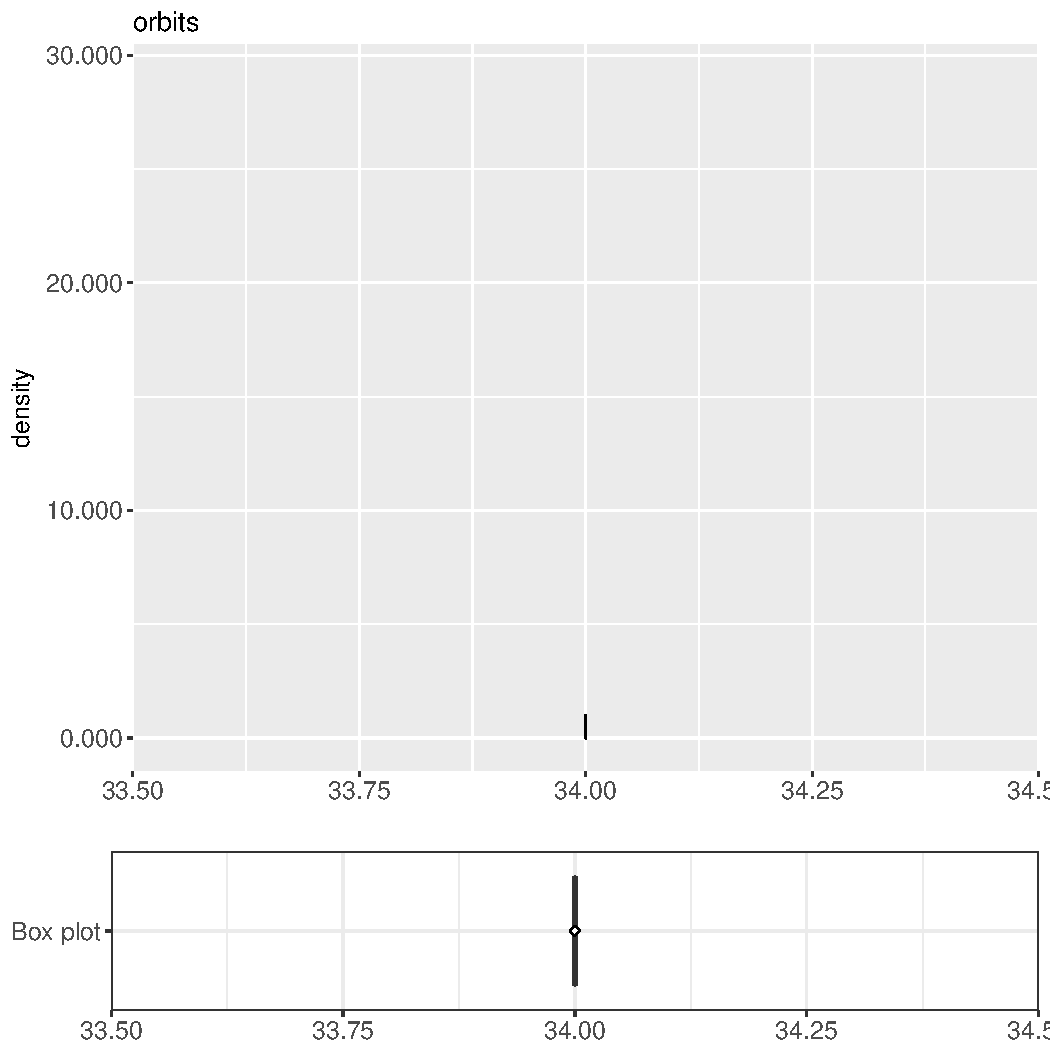
\includegraphics[width=\maxwidth]{figure/RH5_cashew_big-1} 

\end{knitrout}
 \textbf{Number of Orbits for Except order}
\begin{knitrout}
\definecolor{shadecolor}{rgb}{0.969, 0.969, 0.969}\color{fgcolor}\begin{kframe}
\begin{verbatim}
## [1] "Sample size:  1"
##    Min. 1st Qu.  Median    Mean 3rd Qu.    Max. 
##      72      72      72      72      72      72
\end{verbatim}


{\ttfamily\noindent\bfseries\color{errorcolor}{\#\# Error in shapiro.test(subset(json\_data, treatment == "{}cashewExceptOrder"{} \& : sample size must be between 3 and 5000}}\end{kframe}
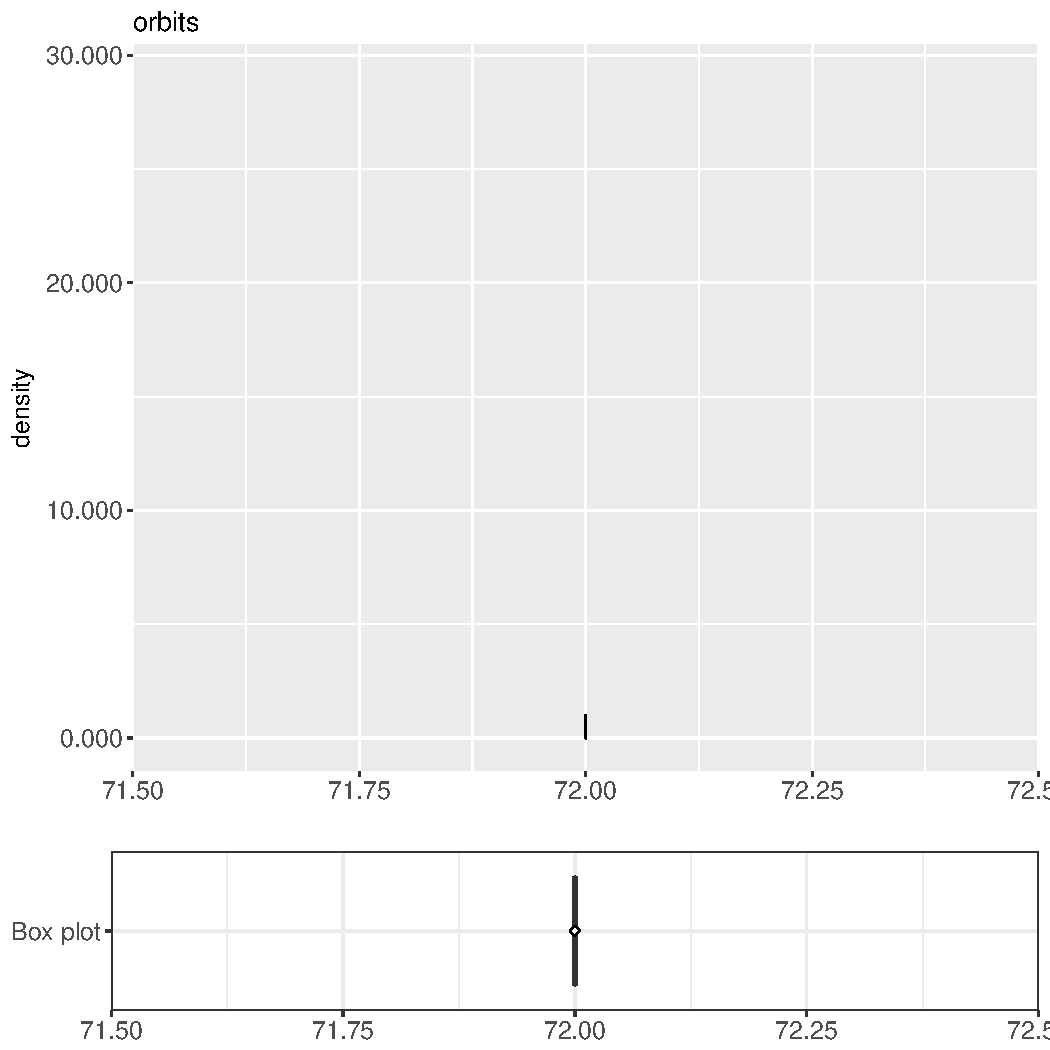
\includegraphics[width=\maxwidth]{figure/RH5_cashewExceptOrder_big-1} 

\end{knitrout}
  
 \textbf{Comparison}
  
\begin{knitrout}
\definecolor{shadecolor}{rgb}{0.969, 0.969, 0.969}\color{fgcolor}
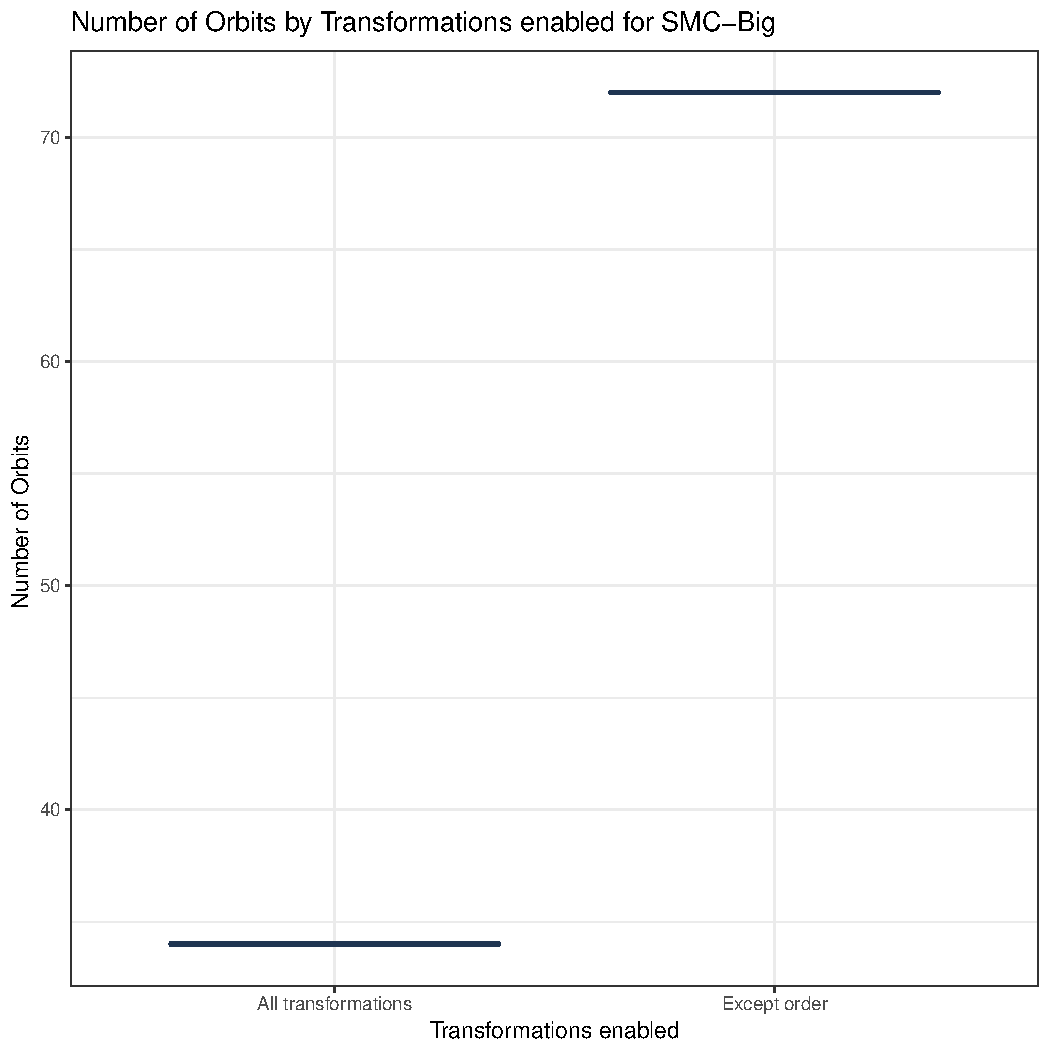
\includegraphics[width=\maxwidth]{figure/RH5_big-1} 
\begin{kframe}

{\ttfamily\noindent\bfseries\color{errorcolor}{\#\# Error in eval(expr, envir, enclos): object 'shap\_cashew\_big' not found}}\begin{verbatim}
## [1] ""
## [1] "Means comparison"
## [1] "Mean Number of Orbits for All transformations:  34"
## [1] "Mean Number of Orbits for Except order:  72"
## [1] "Absolute difference:  38"
## Number of Orbits for Except order is  111.764705882353 % greater than 
## Number of Orbits for All transformations
\end{verbatim}
\end{kframe}
\end{knitrout}


 

	
	\subsubsection{RH5 Results: Number of Orbits All transformations = Except order}
	
	
	\begin{table}[H]
	\centering
	\caption{RH5 Results per Object}
	\begin{tabular}{ll}
	\textbf{SMC-Small} & Inconclusive \\
	\textbf{SMC-Big} & Inconclusive \\
	\end{tabular}
	\end{table}

	\begin{table}[H]
	\centering
	\caption{RH5 Results Summary}
	\begin{tabular}{ll}
	\textbf{All transformations \textless{} Except order:}& 0\% \\
	\textbf{All transformations \textgreater{} Except order:}& 0\%\\
	\textbf{All transformations:} & 0\%\\
	\textbf{Except order:} & 0\%\\
	\textbf{None:}& 0\%\\
	\textbf{Inconclusive:}& 100\%
			
	
	\end{tabular}
	\end{table}
	
	
	



\subsection{RH6: Number of Orbits for Cashew is equals than the Number of Orbits for Cashew Except Reduce}


 
\begin{knitrout}
\definecolor{shadecolor}{rgb}{0.969, 0.969, 0.969}\color{fgcolor}
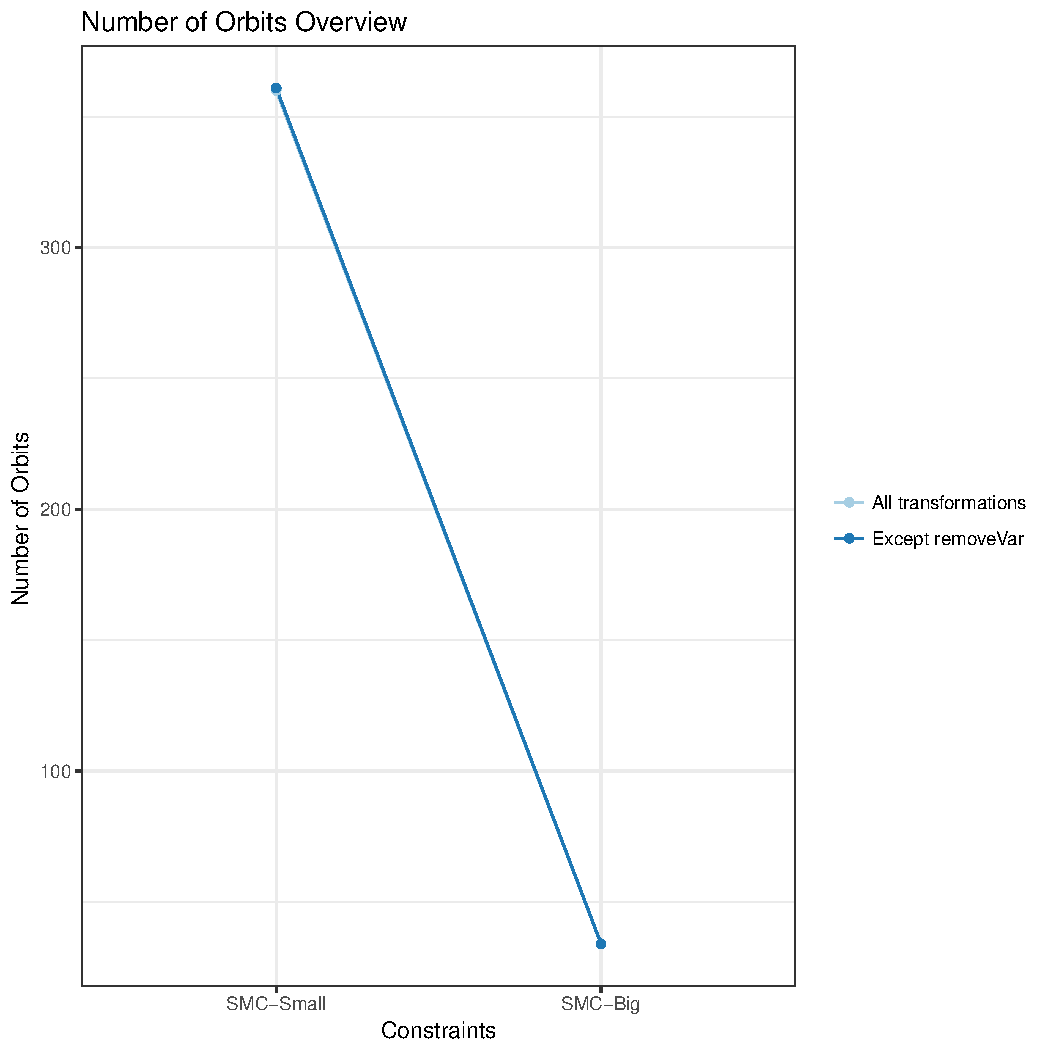
\includegraphics[width=\maxwidth]{figure/overview_RH6-1} 

\end{knitrout}
 	

\subsubsection{RH6.1: Object SMC-Small}

 \textbf{Number of Orbits for All transformations}
\begin{knitrout}
\definecolor{shadecolor}{rgb}{0.969, 0.969, 0.969}\color{fgcolor}\begin{kframe}
\begin{verbatim}
## [1] "Sample size:  1"
##    Min. 1st Qu.  Median    Mean 3rd Qu.    Max. 
##     360     360     360     360     360     360
\end{verbatim}


{\ttfamily\noindent\bfseries\color{errorcolor}{\#\# Error in shapiro.test(subset(json\_data, treatment == "{}cashew"{} \& object == : sample size must be between 3 and 5000}}\end{kframe}
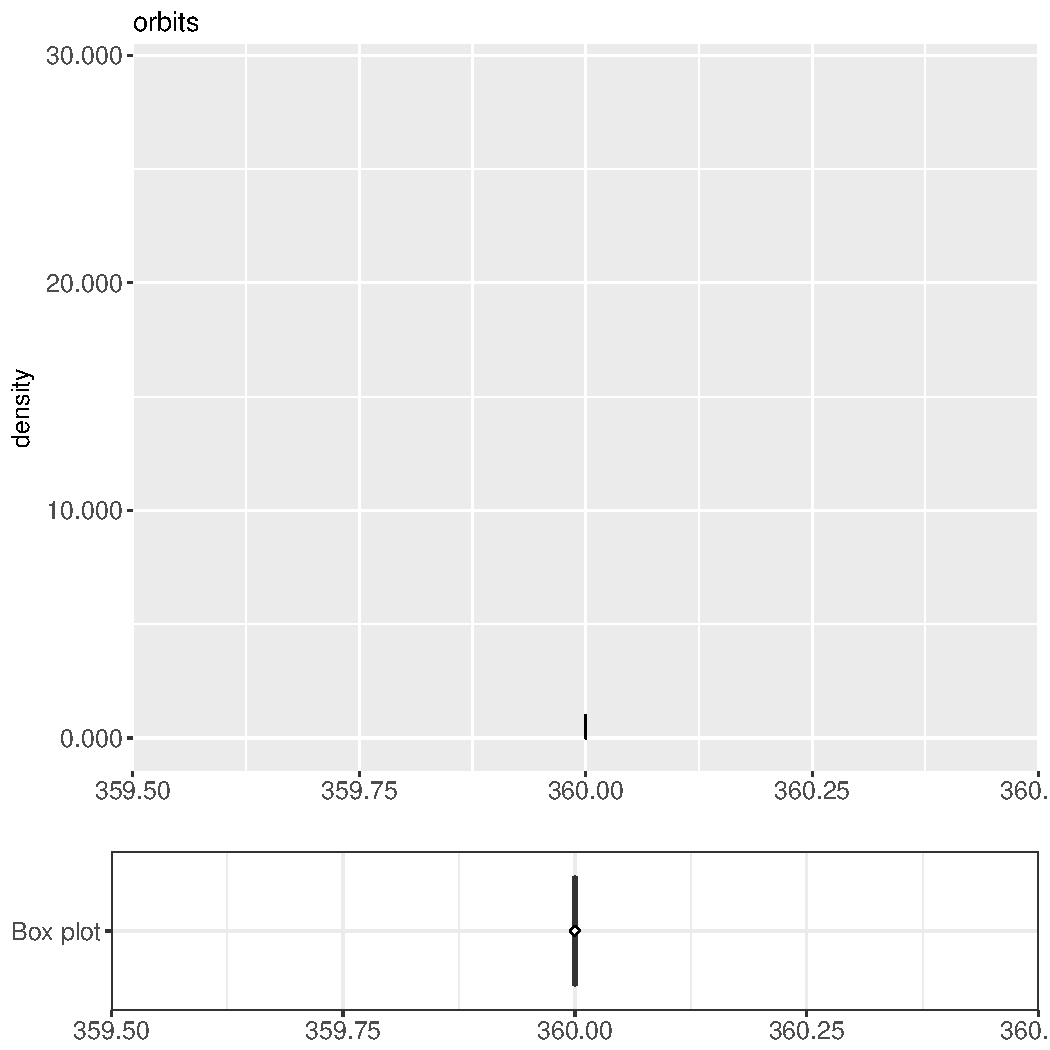
\includegraphics[width=\maxwidth]{figure/RH6_cashew_small-1} 

\end{knitrout}
 \textbf{Number of Orbits for Except removeVar}
\begin{knitrout}
\definecolor{shadecolor}{rgb}{0.969, 0.969, 0.969}\color{fgcolor}\begin{kframe}
\begin{verbatim}
## [1] "Sample size:  1"
##    Min. 1st Qu.  Median    Mean 3rd Qu.    Max. 
##     361     361     361     361     361     361
\end{verbatim}


{\ttfamily\noindent\bfseries\color{errorcolor}{\#\# Error in shapiro.test(subset(json\_data, treatment == "{}cashewExceptReduce"{} \& : sample size must be between 3 and 5000}}\end{kframe}
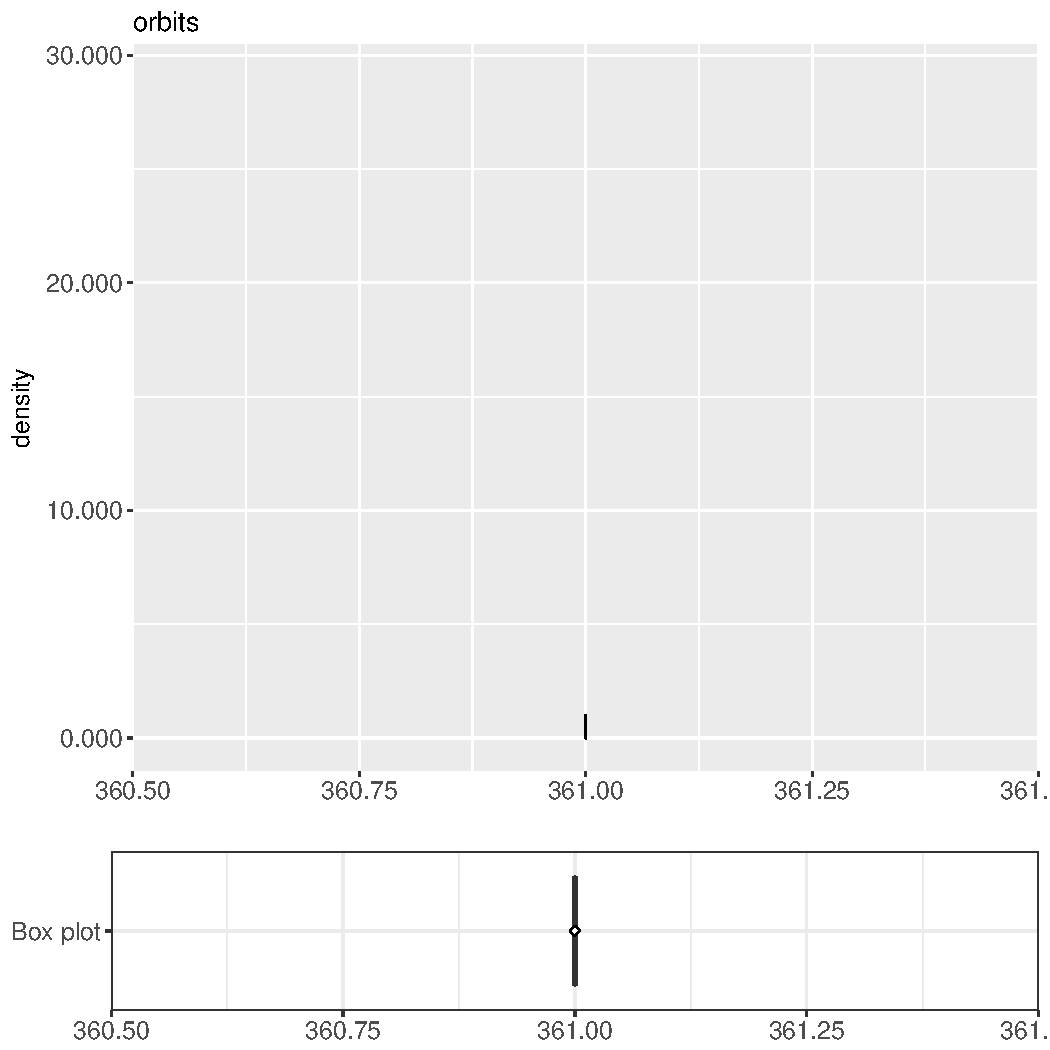
\includegraphics[width=\maxwidth]{figure/RH6_cashewExceptReduce_small-1} 

\end{knitrout}
  
 \textbf{Comparison}
  
\begin{knitrout}
\definecolor{shadecolor}{rgb}{0.969, 0.969, 0.969}\color{fgcolor}
\includegraphics[width=\maxwidth]{figure/RH6_small-1} 
\begin{kframe}

{\ttfamily\noindent\bfseries\color{errorcolor}{\#\# Error in eval(expr, envir, enclos): object 'shap\_cashew\_small' not found}}\begin{verbatim}
## [1] ""
## [1] "Means comparison"
## [1] "Mean Number of Orbits for All transformations:  360"
## [1] "Mean Number of Orbits for Except removeVar:  361"
## [1] "Absolute difference:  1"
## Number of Orbits for Except removeVar is  0.277777777777778 % greater than 
## Number of Orbits for All transformations
\end{verbatim}
\end{kframe}
\end{knitrout}


\subsubsection{RH6.2: Object SMC-Big}

 \textbf{Number of Orbits for All transformations}
\begin{knitrout}
\definecolor{shadecolor}{rgb}{0.969, 0.969, 0.969}\color{fgcolor}\begin{kframe}
\begin{verbatim}
## [1] "Sample size:  1"
##    Min. 1st Qu.  Median    Mean 3rd Qu.    Max. 
##      34      34      34      34      34      34
\end{verbatim}


{\ttfamily\noindent\bfseries\color{errorcolor}{\#\# Error in shapiro.test(subset(json\_data, treatment == "{}cashew"{} \& object == : sample size must be between 3 and 5000}}\end{kframe}
\includegraphics[width=\maxwidth]{figure/RH6_cashew_big-1} 

\end{knitrout}
 \textbf{Number of Orbits for Except removeVar}
\begin{knitrout}
\definecolor{shadecolor}{rgb}{0.969, 0.969, 0.969}\color{fgcolor}\begin{kframe}
\begin{verbatim}
## [1] "Sample size:  1"
##    Min. 1st Qu.  Median    Mean 3rd Qu.    Max. 
##      34      34      34      34      34      34
\end{verbatim}


{\ttfamily\noindent\bfseries\color{errorcolor}{\#\# Error in shapiro.test(subset(json\_data, treatment == "{}cashewExceptReduce"{} \& : sample size must be between 3 and 5000}}\end{kframe}
\includegraphics[width=\maxwidth]{figure/RH6_cashewExceptReduce_big-1} 

\end{knitrout}
  
 \textbf{Comparison}
  
\begin{knitrout}
\definecolor{shadecolor}{rgb}{0.969, 0.969, 0.969}\color{fgcolor}
\includegraphics[width=\maxwidth]{figure/RH6_big-1} 
\begin{kframe}

{\ttfamily\noindent\bfseries\color{errorcolor}{\#\# Error in eval(expr, envir, enclos): object 'shap\_cashew\_big' not found}}\begin{verbatim}
## [1] ""
## [1] "Means comparison"
## [1] "Mean Number of Orbits for All transformations:  34"
## [1] "Mean Number of Orbits for Except removeVar:  34"
## [1] "Absolute difference:  0"
## Number of Orbits for Except removeVar is  0 % greater than 
## Number of Orbits for All transformations
\end{verbatim}
\end{kframe}
\end{knitrout}


 

	
	\subsubsection{RH6 Results: Number of Orbits All transformations = Except removeVar}
	
	
	\begin{table}[H]
	\centering
	\caption{RH6 Results per Object}
	\begin{tabular}{ll}
	\textbf{SMC-Small} & Inconclusive \\
	\textbf{SMC-Big} & Inconclusive \\
	\end{tabular}
	\end{table}

	\begin{table}[H]
	\centering
	\caption{RH6 Results Summary}
	\begin{tabular}{ll}
	\textbf{All transformations \textless{} Except removeVar:}& 0\% \\
	\textbf{All transformations \textgreater{} Except removeVar:}& 0\%\\
	\textbf{All transformations:} & 0\%\\
	\textbf{Except removeVar:} & 0\%\\
	\textbf{None:}& 0\%\\
	\textbf{Inconclusive:}& 100\%
			
	
	\end{tabular}
	\end{table}
	
	
	



\subsection{RH7: Number of Orbits for Cashew is equals than the Number of Orbits for Cashew Except Remove}


 
\begin{knitrout}
\definecolor{shadecolor}{rgb}{0.969, 0.969, 0.969}\color{fgcolor}
\includegraphics[width=\maxwidth]{figure/overview_RH7-1} 

\end{knitrout}
 	

\subsubsection{RH7.1: Object SMC-Small}

 \textbf{Number of Orbits for All transformations}
\begin{knitrout}
\definecolor{shadecolor}{rgb}{0.969, 0.969, 0.969}\color{fgcolor}\begin{kframe}
\begin{verbatim}
## [1] "Sample size:  1"
##    Min. 1st Qu.  Median    Mean 3rd Qu.    Max. 
##     360     360     360     360     360     360
\end{verbatim}


{\ttfamily\noindent\bfseries\color{errorcolor}{\#\# Error in shapiro.test(subset(json\_data, treatment == "{}cashew"{} \& object == : sample size must be between 3 and 5000}}\end{kframe}
\includegraphics[width=\maxwidth]{figure/RH7_cashew_small-1} 

\end{knitrout}
 \textbf{Number of Orbits for Except removeConj}
\begin{knitrout}
\definecolor{shadecolor}{rgb}{0.969, 0.969, 0.969}\color{fgcolor}\begin{kframe}
\begin{verbatim}
## [1] "Sample size:  1"
##    Min. 1st Qu.  Median    Mean 3rd Qu.    Max. 
##     386     386     386     386     386     386
\end{verbatim}


{\ttfamily\noindent\bfseries\color{errorcolor}{\#\# Error in shapiro.test(subset(json\_data, treatment == "{}cashewExceptRemove"{} \& : sample size must be between 3 and 5000}}\end{kframe}
\includegraphics[width=\maxwidth]{figure/RH7_cashewExceptRemove_small-1} 

\end{knitrout}
  
 \textbf{Comparison}
  
\begin{knitrout}
\definecolor{shadecolor}{rgb}{0.969, 0.969, 0.969}\color{fgcolor}
\includegraphics[width=\maxwidth]{figure/RH7_small-1} 
\begin{kframe}

{\ttfamily\noindent\bfseries\color{errorcolor}{\#\# Error in eval(expr, envir, enclos): object 'shap\_cashew\_small' not found}}\begin{verbatim}
## [1] ""
## [1] "Means comparison"
## [1] "Mean Number of Orbits for All transformations:  360"
## [1] "Mean Number of Orbits for Except removeConj:  386"
## [1] "Absolute difference:  26"
## Number of Orbits for Except removeConj is  7.22222222222222 % greater than 
## Number of Orbits for All transformations
\end{verbatim}
\end{kframe}
\end{knitrout}


\subsubsection{RH7.2: Object SMC-Big}

 \textbf{Number of Orbits for All transformations}
\begin{knitrout}
\definecolor{shadecolor}{rgb}{0.969, 0.969, 0.969}\color{fgcolor}\begin{kframe}
\begin{verbatim}
## [1] "Sample size:  1"
##    Min. 1st Qu.  Median    Mean 3rd Qu.    Max. 
##      34      34      34      34      34      34
\end{verbatim}


{\ttfamily\noindent\bfseries\color{errorcolor}{\#\# Error in shapiro.test(subset(json\_data, treatment == "{}cashew"{} \& object == : sample size must be between 3 and 5000}}\end{kframe}
\includegraphics[width=\maxwidth]{figure/RH7_cashew_big-1} 

\end{knitrout}
 \textbf{Number of Orbits for Except removeConj}
\begin{knitrout}
\definecolor{shadecolor}{rgb}{0.969, 0.969, 0.969}\color{fgcolor}\begin{kframe}
\begin{verbatim}
## [1] "Sample size:  1"
##    Min. 1st Qu.  Median    Mean 3rd Qu.    Max. 
##      40      40      40      40      40      40
\end{verbatim}


{\ttfamily\noindent\bfseries\color{errorcolor}{\#\# Error in shapiro.test(subset(json\_data, treatment == "{}cashewExceptRemove"{} \& : sample size must be between 3 and 5000}}\end{kframe}
\includegraphics[width=\maxwidth]{figure/RH7_cashewExceptRemove_big-1} 

\end{knitrout}
  
 \textbf{Comparison}
  
\begin{knitrout}
\definecolor{shadecolor}{rgb}{0.969, 0.969, 0.969}\color{fgcolor}
\includegraphics[width=\maxwidth]{figure/RH7_big-1} 
\begin{kframe}

{\ttfamily\noindent\bfseries\color{errorcolor}{\#\# Error in eval(expr, envir, enclos): object 'shap\_cashew\_big' not found}}\begin{verbatim}
## [1] ""
## [1] "Means comparison"
## [1] "Mean Number of Orbits for All transformations:  34"
## [1] "Mean Number of Orbits for Except removeConj:  40"
## [1] "Absolute difference:  6"
## Number of Orbits for Except removeConj is  17.6470588235294 % greater than 
## Number of Orbits for All transformations
\end{verbatim}
\end{kframe}
\end{knitrout}


 

	
	\subsubsection{RH7 Results: Number of Orbits All transformations = Except removeConj}
	
	
	\begin{table}[H]
	\centering
	\caption{RH7 Results per Object}
	\begin{tabular}{ll}
	\textbf{SMC-Small} & Inconclusive \\
	\textbf{SMC-Big} & Inconclusive \\
	\end{tabular}
	\end{table}

	\begin{table}[H]
	\centering
	\caption{RH7 Results Summary}
	\begin{tabular}{ll}
	\textbf{All transformations \textless{} Except removeConj:}& 0\% \\
	\textbf{All transformations \textgreater{} Except removeConj:}& 0\%\\
	\textbf{All transformations:} & 0\%\\
	\textbf{Except removeConj:} & 0\%\\
	\textbf{None:}& 0\%\\
	\textbf{Inconclusive:}& 100\%
			
	
	\end{tabular}
	\end{table}
	
	
	



\subsection{RH8: Number of Orbits for Cashew is equals than the Number of Orbits for Cashew Except Rename Alph}


 
\begin{knitrout}
\definecolor{shadecolor}{rgb}{0.969, 0.969, 0.969}\color{fgcolor}
\includegraphics[width=\maxwidth]{figure/overview_RH8-1} 

\end{knitrout}
 	

\subsubsection{RH8.1: Object SMC-Small}

 \textbf{Number of Orbits for All transformations}
\begin{knitrout}
\definecolor{shadecolor}{rgb}{0.969, 0.969, 0.969}\color{fgcolor}\begin{kframe}
\begin{verbatim}
## [1] "Sample size:  1"
##    Min. 1st Qu.  Median    Mean 3rd Qu.    Max. 
##     360     360     360     360     360     360
\end{verbatim}


{\ttfamily\noindent\bfseries\color{errorcolor}{\#\# Error in shapiro.test(subset(json\_data, treatment == "{}cashew"{} \& object == : sample size must be between 3 and 5000}}\end{kframe}
\includegraphics[width=\maxwidth]{figure/RH8_cashew_small-1} 

\end{knitrout}
 \textbf{Number of Orbits for Except rename alph}
\begin{knitrout}
\definecolor{shadecolor}{rgb}{0.969, 0.969, 0.969}\color{fgcolor}\begin{kframe}
\begin{verbatim}
## [1] "Sample size:  1"
##    Min. 1st Qu.  Median    Mean 3rd Qu.    Max. 
##     841     841     841     841     841     841
\end{verbatim}


{\ttfamily\noindent\bfseries\color{errorcolor}{\#\# Error in shapiro.test(subset(json\_data, treatment == "{}cashewExceptRenameAlph"{} \& : sample size must be between 3 and 5000}}\end{kframe}
\includegraphics[width=\maxwidth]{figure/RH8_cashewExceptRenameAlph_small-1} 

\end{knitrout}
  
 \textbf{Comparison}
  
\begin{knitrout}
\definecolor{shadecolor}{rgb}{0.969, 0.969, 0.969}\color{fgcolor}
\includegraphics[width=\maxwidth]{figure/RH8_small-1} 
\begin{kframe}

{\ttfamily\noindent\bfseries\color{errorcolor}{\#\# Error in eval(expr, envir, enclos): object 'shap\_cashew\_small' not found}}\begin{verbatim}
## [1] ""
## [1] "Means comparison"
## [1] "Mean Number of Orbits for All transformations:  360"
## [1] "Mean Number of Orbits for Except rename alph:  841"
## [1] "Absolute difference:  481"
## Number of Orbits for Except rename alph is  133.611111111111 % greater than 
## Number of Orbits for All transformations
\end{verbatim}
\end{kframe}
\end{knitrout}


\subsubsection{RH8.2: Object SMC-Big}

 \textbf{Number of Orbits for All transformations}
\begin{knitrout}
\definecolor{shadecolor}{rgb}{0.969, 0.969, 0.969}\color{fgcolor}\begin{kframe}
\begin{verbatim}
## [1] "Sample size:  1"
##    Min. 1st Qu.  Median    Mean 3rd Qu.    Max. 
##      34      34      34      34      34      34
\end{verbatim}


{\ttfamily\noindent\bfseries\color{errorcolor}{\#\# Error in shapiro.test(subset(json\_data, treatment == "{}cashew"{} \& object == : sample size must be between 3 and 5000}}\end{kframe}
\includegraphics[width=\maxwidth]{figure/RH8_cashew_big-1} 

\end{knitrout}
 \textbf{Number of Orbits for Except rename alph}
\begin{knitrout}
\definecolor{shadecolor}{rgb}{0.969, 0.969, 0.969}\color{fgcolor}\begin{kframe}
\begin{verbatim}
## [1] "Sample size:  1"
##    Min. 1st Qu.  Median    Mean 3rd Qu.    Max. 
##      35      35      35      35      35      35
\end{verbatim}


{\ttfamily\noindent\bfseries\color{errorcolor}{\#\# Error in shapiro.test(subset(json\_data, treatment == "{}cashewExceptRenameAlph"{} \& : sample size must be between 3 and 5000}}\end{kframe}
\includegraphics[width=\maxwidth]{figure/RH8_cashewExceptRenameAlph_big-1} 

\end{knitrout}
  
 \textbf{Comparison}
  
\begin{knitrout}
\definecolor{shadecolor}{rgb}{0.969, 0.969, 0.969}\color{fgcolor}
\includegraphics[width=\maxwidth]{figure/RH8_big-1} 
\begin{kframe}

{\ttfamily\noindent\bfseries\color{errorcolor}{\#\# Error in eval(expr, envir, enclos): object 'shap\_cashew\_big' not found}}\begin{verbatim}
## [1] ""
## [1] "Means comparison"
## [1] "Mean Number of Orbits for All transformations:  34"
## [1] "Mean Number of Orbits for Except rename alph:  35"
## [1] "Absolute difference:  1"
## Number of Orbits for Except rename alph is  2.94117647058824 % greater than 
## Number of Orbits for All transformations
\end{verbatim}
\end{kframe}
\end{knitrout}


 

	
	\subsubsection{RH8 Results: Number of Orbits All transformations = Except rename alph}
	
	
	\begin{table}[H]
	\centering
	\caption{RH8 Results per Object}
	\begin{tabular}{ll}
	\textbf{SMC-Small} & Inconclusive \\
	\textbf{SMC-Big} & Inconclusive \\
	\end{tabular}
	\end{table}

	\begin{table}[H]
	\centering
	\caption{RH8 Results Summary}
	\begin{tabular}{ll}
	\textbf{All transformations \textless{} Except rename alph:}& 0\% \\
	\textbf{All transformations \textgreater{} Except rename alph:}& 0\%\\
	\textbf{All transformations:} & 0\%\\
	\textbf{Except rename alph:} & 0\%\\
	\textbf{None:}& 0\%\\
	\textbf{Inconclusive:}& 100\%
			
	
	\end{tabular}
	\end{table}
	
	
	



\subsection{RH9: Number of Orbits for Cashew is equals than the Number of Orbits for Cashew Except Rename Var}


 
\begin{knitrout}
\definecolor{shadecolor}{rgb}{0.969, 0.969, 0.969}\color{fgcolor}
\includegraphics[width=\maxwidth]{figure/overview_RH9-1} 

\end{knitrout}
 	

\subsubsection{RH9.1: Object SMC-Small}

 \textbf{Number of Orbits for All transformations}
\begin{knitrout}
\definecolor{shadecolor}{rgb}{0.969, 0.969, 0.969}\color{fgcolor}\begin{kframe}
\begin{verbatim}
## [1] "Sample size:  1"
##    Min. 1st Qu.  Median    Mean 3rd Qu.    Max. 
##     360     360     360     360     360     360
\end{verbatim}


{\ttfamily\noindent\bfseries\color{errorcolor}{\#\# Error in shapiro.test(subset(json\_data, treatment == "{}cashew"{} \& object == : sample size must be between 3 and 5000}}\end{kframe}
\includegraphics[width=\maxwidth]{figure/RH9_cashew_small-1} 

\end{knitrout}
 \textbf{Number of Orbits for Except rename var}
\begin{knitrout}
\definecolor{shadecolor}{rgb}{0.969, 0.969, 0.969}\color{fgcolor}\begin{kframe}
\begin{verbatim}
## [1] "Sample size:  1"
##    Min. 1st Qu.  Median    Mean 3rd Qu.    Max. 
##    9645    9645    9645    9645    9645    9645
\end{verbatim}


{\ttfamily\noindent\bfseries\color{errorcolor}{\#\# Error in shapiro.test(subset(json\_data, treatment == "{}cashewExceptRenameVar"{} \& : sample size must be between 3 and 5000}}\end{kframe}
\includegraphics[width=\maxwidth]{figure/RH9_cashewExceptRenameVar_small-1} 

\end{knitrout}
  
 \textbf{Comparison}
  
\begin{knitrout}
\definecolor{shadecolor}{rgb}{0.969, 0.969, 0.969}\color{fgcolor}
\includegraphics[width=\maxwidth]{figure/RH9_small-1} 
\begin{kframe}

{\ttfamily\noindent\bfseries\color{errorcolor}{\#\# Error in eval(expr, envir, enclos): object 'shap\_cashew\_small' not found}}\begin{verbatim}
## [1] ""
## [1] "Means comparison"
## [1] "Mean Number of Orbits for All transformations:  360"
## [1] "Mean Number of Orbits for Except rename var:  9645"
## [1] "Absolute difference:  9285"
## Number of Orbits for Except rename var is  2579.16666666667 % greater than 
## Number of Orbits for All transformations
\end{verbatim}
\end{kframe}
\end{knitrout}


\subsubsection{RH9.2: Object SMC-Big}

 \textbf{Number of Orbits for All transformations}
\begin{knitrout}
\definecolor{shadecolor}{rgb}{0.969, 0.969, 0.969}\color{fgcolor}\begin{kframe}
\begin{verbatim}
## [1] "Sample size:  1"
##    Min. 1st Qu.  Median    Mean 3rd Qu.    Max. 
##      34      34      34      34      34      34
\end{verbatim}


{\ttfamily\noindent\bfseries\color{errorcolor}{\#\# Error in shapiro.test(subset(json\_data, treatment == "{}cashew"{} \& object == : sample size must be between 3 and 5000}}\end{kframe}
\includegraphics[width=\maxwidth]{figure/RH9_cashew_big-1} 

\end{knitrout}
 \textbf{Number of Orbits for Except rename var}
\begin{knitrout}
\definecolor{shadecolor}{rgb}{0.969, 0.969, 0.969}\color{fgcolor}\begin{kframe}
\begin{verbatim}
## [1] "Sample size:  1"
##    Min. 1st Qu.  Median    Mean 3rd Qu.    Max. 
##     344     344     344     344     344     344
\end{verbatim}


{\ttfamily\noindent\bfseries\color{errorcolor}{\#\# Error in shapiro.test(subset(json\_data, treatment == "{}cashewExceptRenameVar"{} \& : sample size must be between 3 and 5000}}\end{kframe}
\includegraphics[width=\maxwidth]{figure/RH9_cashewExceptRenameVar_big-1} 

\end{knitrout}
  
 \textbf{Comparison}
  
\begin{knitrout}
\definecolor{shadecolor}{rgb}{0.969, 0.969, 0.969}\color{fgcolor}
\includegraphics[width=\maxwidth]{figure/RH9_big-1} 
\begin{kframe}

{\ttfamily\noindent\bfseries\color{errorcolor}{\#\# Error in eval(expr, envir, enclos): object 'shap\_cashew\_big' not found}}\begin{verbatim}
## [1] ""
## [1] "Means comparison"
## [1] "Mean Number of Orbits for All transformations:  34"
## [1] "Mean Number of Orbits for Except rename var:  344"
## [1] "Absolute difference:  310"
## Number of Orbits for Except rename var is  911.764705882353 % greater than 
## Number of Orbits for All transformations
\end{verbatim}
\end{kframe}
\end{knitrout}


 

	
	\subsubsection{RH9 Results: Number of Orbits All transformations = Except rename var}
	
	
	\begin{table}[H]
	\centering
	\caption{RH9 Results per Object}
	\begin{tabular}{ll}
	\textbf{SMC-Small} & Inconclusive \\
	\textbf{SMC-Big} & Inconclusive \\
	\end{tabular}
	\end{table}

	\begin{table}[H]
	\centering
	\caption{RH9 Results Summary}
	\begin{tabular}{ll}
	\textbf{All transformations \textless{} Except rename var:}& 0\% \\
	\textbf{All transformations \textgreater{} Except rename var:}& 0\%\\
	\textbf{All transformations:} & 0\%\\
	\textbf{Except rename var:} & 0\%\\
	\textbf{None:}& 0\%\\
	\textbf{Inconclusive:}& 100\%
			
	
	\end{tabular}
	\end{table}
	
	
	



\section{Result Summary}
\subsection{Research Hypotheses}


	
	\subsubsection{RH1 Results: Average time All transformations = No cache}
	
	
	\begin{table}[H]
	\centering
	\caption{RH1 Results per Object}
	\begin{tabular}{ll}
	\textbf{SMC-Small} & Inconclusive \\
	\textbf{SMC-Big} & Inconclusive \\
	\end{tabular}
	\end{table}

	\begin{table}[H]
	\centering
	\caption{RH1 Results Summary}
	\begin{tabular}{ll}
	\textbf{All transformations \textless{} No cache:}& 0\% \\
	\textbf{All transformations \textgreater{} No cache:}& 0\%\\
	\textbf{All transformations:} & 0\%\\
	\textbf{No cache:} & 0\%\\
	\textbf{None:}& 0\%\\
	\textbf{Inconclusive:}& 100\%
			
	
	\end{tabular}
	\end{table}
	
	
	

	
	\subsubsection{RH2 Results: Maximum time All transformations = No cache}
	
	
	\begin{table}[H]
	\centering
	\caption{RH2 Results per Object}
	\begin{tabular}{ll}
	\textbf{SMC-Small} & Inconclusive \\
	\textbf{SMC-Big} & Inconclusive \\
	\end{tabular}
	\end{table}

	\begin{table}[H]
	\centering
	\caption{RH2 Results Summary}
	\begin{tabular}{ll}
	\textbf{All transformations \textless{} No cache:}& 0\% \\
	\textbf{All transformations \textgreater{} No cache:}& 0\%\\
	\textbf{All transformations:} & 0\%\\
	\textbf{No cache:} & 0\%\\
	\textbf{None:}& 0\%\\
	\textbf{Inconclusive:}& 100\%
			
	
	\end{tabular}
	\end{table}
	
	
	

	
	\subsubsection{RH3 Results: Total time All transformations = No cache}
	
	
	\begin{table}[H]
	\centering
	\caption{RH3 Results per Object}
	\begin{tabular}{ll}
	\textbf{SMC-Small} & Inconclusive \\
	\textbf{SMC-Big} & Inconclusive \\
	\end{tabular}
	\end{table}

	\begin{table}[H]
	\centering
	\caption{RH3 Results Summary}
	\begin{tabular}{ll}
	\textbf{All transformations \textless{} No cache:}& 0\% \\
	\textbf{All transformations \textgreater{} No cache:}& 0\%\\
	\textbf{All transformations:} & 0\%\\
	\textbf{No cache:} & 0\%\\
	\textbf{None:}& 0\%\\
	\textbf{Inconclusive:}& 100\%
			
	
	\end{tabular}
	\end{table}
	
	
	

	
	\subsubsection{RH4 Results: Number of Orbits All transformations = No cache}
	
	
	\begin{table}[H]
	\centering
	\caption{RH4 Results per Object}
	\begin{tabular}{ll}
	\textbf{SMC-Small} & Inconclusive \\
	\textbf{SMC-Big} & Inconclusive \\
	\end{tabular}
	\end{table}

	\begin{table}[H]
	\centering
	\caption{RH4 Results Summary}
	\begin{tabular}{ll}
	\textbf{All transformations \textless{} No cache:}& 0\% \\
	\textbf{All transformations \textgreater{} No cache:}& 0\%\\
	\textbf{All transformations:} & 0\%\\
	\textbf{No cache:} & 0\%\\
	\textbf{None:}& 0\%\\
	\textbf{Inconclusive:}& 100\%
			
	
	\end{tabular}
	\end{table}
	
	
	

	
	\subsubsection{RH5 Results: Number of Orbits All transformations = Except order}
	
	
	\begin{table}[H]
	\centering
	\caption{RH5 Results per Object}
	\begin{tabular}{ll}
	\textbf{SMC-Small} & Inconclusive \\
	\textbf{SMC-Big} & Inconclusive \\
	\end{tabular}
	\end{table}

	\begin{table}[H]
	\centering
	\caption{RH5 Results Summary}
	\begin{tabular}{ll}
	\textbf{All transformations \textless{} Except order:}& 0\% \\
	\textbf{All transformations \textgreater{} Except order:}& 0\%\\
	\textbf{All transformations:} & 0\%\\
	\textbf{Except order:} & 0\%\\
	\textbf{None:}& 0\%\\
	\textbf{Inconclusive:}& 100\%
			
	
	\end{tabular}
	\end{table}
	
	
	

	
	\subsubsection{RH6 Results: Number of Orbits All transformations = Except removeVar}
	
	
	\begin{table}[H]
	\centering
	\caption{RH6 Results per Object}
	\begin{tabular}{ll}
	\textbf{SMC-Small} & Inconclusive \\
	\textbf{SMC-Big} & Inconclusive \\
	\end{tabular}
	\end{table}

	\begin{table}[H]
	\centering
	\caption{RH6 Results Summary}
	\begin{tabular}{ll}
	\textbf{All transformations \textless{} Except removeVar:}& 0\% \\
	\textbf{All transformations \textgreater{} Except removeVar:}& 0\%\\
	\textbf{All transformations:} & 0\%\\
	\textbf{Except removeVar:} & 0\%\\
	\textbf{None:}& 0\%\\
	\textbf{Inconclusive:}& 100\%
			
	
	\end{tabular}
	\end{table}
	
	
	

	
	\subsubsection{RH7 Results: Number of Orbits All transformations = Except removeConj}
	
	
	\begin{table}[H]
	\centering
	\caption{RH7 Results per Object}
	\begin{tabular}{ll}
	\textbf{SMC-Small} & Inconclusive \\
	\textbf{SMC-Big} & Inconclusive \\
	\end{tabular}
	\end{table}

	\begin{table}[H]
	\centering
	\caption{RH7 Results Summary}
	\begin{tabular}{ll}
	\textbf{All transformations \textless{} Except removeConj:}& 0\% \\
	\textbf{All transformations \textgreater{} Except removeConj:}& 0\%\\
	\textbf{All transformations:} & 0\%\\
	\textbf{Except removeConj:} & 0\%\\
	\textbf{None:}& 0\%\\
	\textbf{Inconclusive:}& 100\%
			
	
	\end{tabular}
	\end{table}
	
	
	

	
	\subsubsection{RH8 Results: Number of Orbits All transformations = Except rename alph}
	
	
	\begin{table}[H]
	\centering
	\caption{RH8 Results per Object}
	\begin{tabular}{ll}
	\textbf{SMC-Small} & Inconclusive \\
	\textbf{SMC-Big} & Inconclusive \\
	\end{tabular}
	\end{table}

	\begin{table}[H]
	\centering
	\caption{RH8 Results Summary}
	\begin{tabular}{ll}
	\textbf{All transformations \textless{} Except rename alph:}& 0\% \\
	\textbf{All transformations \textgreater{} Except rename alph:}& 0\%\\
	\textbf{All transformations:} & 0\%\\
	\textbf{Except rename alph:} & 0\%\\
	\textbf{None:}& 0\%\\
	\textbf{Inconclusive:}& 100\%
			
	
	\end{tabular}
	\end{table}
	
	
	

	
	\subsubsection{RH9 Results: Number of Orbits All transformations = Except rename var}
	
	
	\begin{table}[H]
	\centering
	\caption{RH9 Results per Object}
	\begin{tabular}{ll}
	\textbf{SMC-Small} & Inconclusive \\
	\textbf{SMC-Big} & Inconclusive \\
	\end{tabular}
	\end{table}

	\begin{table}[H]
	\centering
	\caption{RH9 Results Summary}
	\begin{tabular}{ll}
	\textbf{All transformations \textless{} Except rename var:}& 0\% \\
	\textbf{All transformations \textgreater{} Except rename var:}& 0\%\\
	\textbf{All transformations:} & 0\%\\
	\textbf{Except rename var:} & 0\%\\
	\textbf{None:}& 0\%\\
	\textbf{Inconclusive:}& 100\%
			
	
	\end{tabular}
	\end{table}
	
	
	
		


	
\clearpage
\appendix
\section{Session Information}
\begin{knitrout}
\definecolor{shadecolor}{rgb}{0.969, 0.969, 0.969}\color{fgcolor}\begin{kframe}
\begin{verbatim}
## R version 3.3.1 (2016-06-21)
## Platform: x86_64-pc-linux-gnu (64-bit)
## Running under: Ubuntu 16.10
## 
## locale:
##  [1] LC_CTYPE=pt_BR.UTF-8       LC_NUMERIC=C              
##  [3] LC_TIME=pt_BR.UTF-8        LC_COLLATE=en_US.UTF-8    
##  [5] LC_MONETARY=pt_BR.UTF-8    LC_MESSAGES=en_US.UTF-8   
##  [7] LC_PAPER=pt_BR.UTF-8       LC_NAME=C                 
##  [9] LC_ADDRESS=C               LC_TELEPHONE=C            
## [11] LC_MEASUREMENT=pt_BR.UTF-8 LC_IDENTIFICATION=C       
## 
## attached base packages:
## [1] stats     graphics  grDevices utils     datasets  methods   base     
## 
## other attached packages:
## [1] plyr_1.8.4       jsonlite_1.5     ggplot2_2.2.1    reproducer_0.1.8
## [5] knitr_1.17      
## 
## loaded via a namespace (and not attached):
##  [1] Rcpp_0.12.16       digest_0.6.12      grid_3.3.1        
##  [4] gtable_0.2.0       magrittr_1.5       evaluate_0.10     
##  [7] scales_0.4.1       rlang_0.2.0        stringi_1.1.5     
## [10] lazyeval_0.2.0     labeling_0.3       RColorBrewer_1.1-2
## [13] tools_3.3.1        stringr_1.2.0      munsell_0.4.3     
## [16] colorspace_1.3-2   gridExtra_2.2.1    tibble_1.3.1
\end{verbatim}
\end{kframe}
\end{knitrout}

\end{document}
